% Chinese reading copy: make pdf-zh (XeLaTeX).
% Chapters 5 and 7 are translated; other unfinished text remains a skeleton.
\documentclass[a4paper,12pt,oneside,openany]{report}

% Thesis identity and submission layout settings.
\newcommand{\thesistitle}{JHQ-GPU: Representation-Aware GPU ANN Search and Workload-Level Refinement Calibration}
\newcommand{\thesisshorttitle}{JHQ-GPU}
\newcommand{\thesissubtitle}{Representation-Aware GPU ANN Search\\and Workload-Level Refinement Calibration}
\newcommand{\thesisauthor}{Rui Luo}
\newcommand{\thesissupervisor}{Dr Mengxuan Zhang}
\newcommand{\thesiscourse}{COMP8800 --- Advanced Computing Research Project}
\newcommand{\thesisschool}{School of Computing}
\newcommand{\thesisuniversity}{The Australian National University}
\newcommand{\thesisdate}{October 2026}
% Optional: enter your student number if required by Canvas; blank hides it.
\newcommand{\thesisstudentnumber}{}

% The final build rejects unresolved writing or figure placeholders.
\newif\ifdraftthesis
\draftthesisfalse

\renewcommand{\thesistitle}{JHQ-GPU：面向表示的 GPU 近似最近邻搜索与工作负载级精排预算校准}
% Chinese reading copy of the documented School of Computing long-thesis adaptation.
\usepackage{fontspec}
\usepackage{xeCJK}
\setmainfont{lmroman10-regular.otf}[
  BoldFont=lmroman10-bold.otf,
  ItalicFont=lmroman10-italic.otf,
  BoldItalicFont=lmroman10-bolditalic.otf]
\setsansfont{lmsans10-regular.otf}[
  BoldFont=lmsans10-bold.otf,
  ItalicFont=lmsans10-oblique.otf,
  BoldItalicFont=lmsans10-boldoblique.otf]
\setmonofont{lmmono10-regular.otf}[
  BoldFont=lmmonolt10-bold.otf,
  ItalicFont=lmmono10-italic.otf,
  BoldItalicFont=lmmonolt10-boldoblique.otf]
\setCJKmainfont{FandolSong-Regular.otf}[
  BoldFont=FandolSong-Bold.otf,
  ItalicFont=FandolKai-Regular.otf]
\setCJKsansfont{FandolHei-Regular.otf}[BoldFont=FandolHei-Bold.otf]
\setCJKmonofont{FandolFang-Regular.otf}
\XeTeXlinebreaklocale "zh"
\XeTeXlinebreakskip=0pt plus 1pt
\usepackage{microtype}
\usepackage{geometry}
\usepackage{setspace}
\usepackage{xcolor}
\definecolor{ThesisNavy}{HTML}{18344A}
\definecolor{DraftColour}{HTML}{8A4515}
\usepackage{graphicx}
\graphicspath{{figures/}}
\usepackage{amsmath,amssymb,amsthm}
\usepackage{booktabs,array,tabularx,longtable}
\usepackage{caption,subcaption}
\captionsetup{font=small,labelfont=bf}
\captionsetup[table]{position=top}
\usepackage{enumitem}
\setlist{itemsep=0.2em,topsep=0.35em}
\usepackage{listings}
\lstset{basicstyle=\small\ttfamily,breaklines=true,
  columns=fullflexible,keepspaces=true,showstringspaces=false,
  frame=single,rulecolor=\color{black!20},tabsize=2}
\usepackage{tikz}
\usetikzlibrary{arrows.meta,positioning,decorations.pathreplacing}
\usepackage[numbers,sort&compress]{natbib}
\usepackage[automark,headsepline]{scrlayer-scrpage}
% KOMA-Script long-thesis adaptation; see FORMAT_NOTES.txt for the ANU source.
% Independently configured with public KOMA interfaces; no third-party template source is redistributed.
% Keep the existing font size and margins. Normal leading follows the school template.
\geometry{a4paper,left=27mm,right=27mm,top=28mm,bottom=28mm,
  headheight=18pt,headsep=7mm,footskip=12mm}
\setstretch{1.0}
% Classic thesis paragraphs: indent instead of a half-line blank between them.
\setparsizes{1.2em}{0pt plus .5pt}{0pt plus 1fil}
% Preserve the existing, scoped roman math subscripts without rewriting equations.
\DeclareOldFontCommand{\rm}{\normalfont\rmfamily}{\mathrm}

% Mathematical statements and proofs share the body-text margins. Their
% headings occupy a separate line; upright statements distinguish prose from
% the mathematical symbols without switching whole paragraphs to italics.
\newtheoremstyle{thesis}
  {6pt plus 1pt minus 1pt}{4pt plus 1pt minus 1pt}
  {\normalfont\setlength{\parindent}{0pt}}{0pt}
  {\normalfont\bfseries}{.}{\newline}{}
\theoremstyle{thesis}
\makeatletter
\renewenvironment{proof}[1][\proofname]{%
  \par\pushQED{\qed}\normalfont
  \setlength{\parindent}{0pt}\setlength{\listparindent}{0pt}%
  \setlength{\parskip}{2pt plus .5pt}%
  \topsep4\p@\@plus\p@\@minus\p@\relax
  \trivlist
  \item[\hskip\labelsep\normalfont\bfseries #1\@addpunct{.}]%
  \leavevmode\par\nobreak\noindent\ignorespaces
}{%
  \popQED\endtrivlist\@endpefalse
}
\makeatother
% Each current statement/proof pair fits comfortably on one page. Keep the
% short pairs together so floats and page breaks cannot separate their parts.
\newenvironment{resultblock}{%
  \par\addvspace{6pt}\noindent\begin{minipage}[t]{\linewidth}%
}{%
  \end{minipage}\par\addvspace{6pt}%
}

\KOMAoptions{chapterprefix=false,headings=normal,numbers=noendperiod}
\setkomafont{disposition}{\normalfont\bfseries}
\setkomafont{chapter}{\normalfont\Large\bfseries}
\setkomafont{chapterprefix}{\normalfont\large\bfseries}
\RedeclareSectionCommand[beforeskip=1.5ex plus .3ex minus .2ex,
  afterskip=.8ex plus .2ex]{chapter}
\RedeclareSectionCommand[beforeskip=1.8ex plus .4ex minus .2ex,
  afterskip=.7ex plus .2ex]{section}
\RedeclareSectionCommand[beforeskip=1.4ex plus .3ex minus .2ex,
  afterskip=.6ex plus .2ex]{subsection}
\RedeclareSectionCommand[runin=true,beforeskip=.9ex plus .3ex minus .1ex,
  afterskip=.75em]{paragraph}

\clearpairofpagestyles
\automark[chapter]{chapter}
\ihead{\headmark}
\cfoot[\pagemark]{\pagemark}
\setkomafont{pageheadfoot}{\normalfont\footnotesize\color{black!65}}
\setkomafont{pagenumber}{\normalfont\small\color{black}}
\pagestyle{scrheadings}

\captionsetup{font={small,stretch=1.0},labelfont=bf,labelsep=period,
  justification=raggedright,singlelinecheck=false,skip=5pt}
\captionsetup[table]{position=top,skip=4pt}
\setlength{\textfloatsep}{12pt plus 2pt minus 2pt}
\setlength{\floatsep}{10pt plus 2pt minus 2pt}
\setlength{\intextsep}{10pt plus 2pt minus 2pt}
% Keep neighbouring floats together on float-only pages.
\makeatletter
\setlength{\@fptop}{0pt}
\setlength{\@fpsep}{12pt plus 2pt minus 2pt}
\setlength{\@fpbot}{0pt plus 1fil}
\makeatother
\setlength{\abovecaptionskip}{5pt}
\setlength{\belowcaptionskip}{0pt}
\setlist{itemsep=.15em,topsep=.35em,parsep=0pt}
\setlength{\bibsep}{.3em}
\setlength{\abovedisplayskip}{8pt plus 2pt minus 2pt}
\setlength{\belowdisplayskip}{8pt plus 2pt minus 2pt}
\setlength{\abovedisplayshortskip}{4pt plus 1pt}
\setlength{\belowdisplayshortskip}{5pt plus 1pt minus 1pt}
\AtBeginDocument{%
  \setlength{\abovedisplayskip}{8pt plus 2pt minus 2pt}%
  \setlength{\belowdisplayskip}{8pt plus 2pt minus 2pt}%
  \setlength{\abovedisplayshortskip}{4pt plus 1pt}%
  \setlength{\belowdisplayshortskip}{5pt plus 1pt minus 1pt}}

% Short preliminary sections may share a page; numbered chapters stay separate.
\newcommand{\frontsection}[1]{%
  \section*{#1}\phantomsection\addcontentsline{toc}{chapter}{#1}%
  \markboth{#1}{#1}}

% Native KOMA contents/list styles and appendix terminology.
\DeclareTOCStyleEntry[beforeskip=.5em plus .1em]{chapter}{chapter}
\DeclareTOCStyleEntries[pagenumberwidth=2.5em]{chapter}{chapter}
\DeclareTOCStyleEntry[indent=0pt,numwidth=2.8em]{tocline}{figure}
\DeclareTOCStyleEntry[indent=0pt,numwidth=2.8em]{tocline}{table}
\AddToHook{cmd/appendix/after}{\crefalias{chapter}{appendix}}

% Chinese characters need slightly more leading than the Latin reading copy.
\setstretch{1.25}
\setparsizes{2em}{0pt plus .5pt}{0pt plus 1fil}
\renewcommand*{\chapterformat}{第\thechapter 章}
\renewcommand*{\chaptermarkformat}{第\thechapter 章\enskip}
\AddToHook{cmd/appendix/after}{%
  \renewcommand*{\chapterformat}{附录~\thechapter}%
  \renewcommand*{\chaptermarkformat}{附录~\thechapter\enskip}}
\setcounter{secnumdepth}{2}
\setcounter{tocdepth}{1}
\setlength{\emergencystretch}{2em}
\widowpenalty=10000
\clubpenalty=10000
\raggedbottom
% Match the English thesis's result-figure placement.
\renewcommand{\topfraction}{0.90}
\renewcommand{\bottomfraction}{0.85}
\renewcommand{\textfraction}{0.10}
\renewcommand{\floatpagefraction}{0.75}
\setcounter{topnumber}{3}
\setcounter{totalnumber}{4}
\makeatletter
\setlength{\@fptop}{0pt}
\makeatother
\usepackage[hyphens]{url}
\usepackage[unicode,hidelinks,pdfusetitle]{hyperref}
\hypersetup{pdftitle={\thesistitle},pdfauthor={\thesisauthor},
  pdfsubject={COMP8800 research thesis},bookmarksnumbered=true}
\usepackage[nameinlink,noabbrev]{cleveref}

\newtheorem{proposition}{命题}[chapter]
\newtheorem{lemma}{引理}[chapter]
\newtheorem{corollary}[proposition]{推论}
\crefname{corollary}{推论}{推论}
\Crefname{corollary}{推论}{推论}
\theoremstyle{definition}
\newtheorem{definition}[proposition]{定义}
\renewcommand{\proofname}{证明}

\newcommand{\frontchapter}[1]{%
  \chapter*{#1}\phantomsection\addcontentsline{toc}{chapter}{#1}
  \markboth{#1}{#1}}
\newcommand{\draftnote}[1]{%
  \ifdraftthesis
    \par\begingroup\small\color{DraftColour}
    \noindent\textbf{待撰写：} #1\par\endgroup\medskip
  \else
    \PackageError{comp8800-template}{Unresolved writing placeholder}
      {Replace all draftnote commands before a final build.}
  \fi}
\newcommand{\figureplaceholder}[3]{%
  \ifdraftthesis
    \begin{figure}[tbp]\centering
      \fbox{\parbox[c][35mm][c]{0.87\linewidth}{\centering\small #1}}
      \caption{\textbf{Draft placeholder.} #2}\label{#3}
    \end{figure}
  \else
    \PackageError{comp8800-template}{Unresolved figure placeholder}
      {Replace figureplaceholder with the final figure.}
  \fi}
\DeclareMathOperator{\Recall}{Recall}
\newcommand{\rawdist}{D_{\mathrm{raw}}}
\newcommand{\primarydist}{D_{\mathrm{P}}}
\newcommand{\refineddist}{D_{\mathrm{H}}}
\newcommand{\glut}{g_{\mathrm{LUT}}}
\newcommand{\gscan}{g_{\mathrm{scan}}}
\newcommand{\lrefine}{\ell_{\mathrm{ref}}}

% Chinese reading-copy names; labels and numbering follow the English draft.
\renewcommand{\bibfont}{\raggedright}
\crefname{figure}{图}{图}
\Crefname{figure}{图}{图}
\crefname{table}{表}{表}
\Crefname{table}{表}{表}
\crefname{proposition}{命题}{命题}
\Crefname{proposition}{命题}{命题}
\crefname{lemma}{引理}{引理}
\Crefname{lemma}{引理}{引理}
\crefname{appendix}{附录}{附录}
\Crefname{appendix}{附录}{附录}
\crefformat{appendix}{附录~#2#1#3}
\Crefformat{appendix}{附录~#2#1#3}
\crefformat{chapter}{第#2#1#3章}
\Crefformat{chapter}{第#2#1#3章}
\crefformat{section}{第#2#1#3节}
\Crefformat{section}{第#2#1#3节}
\crefformat{equation}{式~(#2#1#3)}
\Crefformat{equation}{式~(#2#1#3)}
\AtBeginDocument{%
  \renewcommand{\contentsname}{目录}%
  \renewcommand{\listfigurename}{插图目录}%
  \renewcommand{\listtablename}{表格目录}%
  \renewcommand{\figurename}{图}%
  \renewcommand{\tablename}{表}%
  \renewcommand{\bibname}{参考文献}%
  \renewcommand{\appendixname}{附录}%
  \renewcommand{\crefpairconjunction}{与}%
  \renewcommand{\crefmiddleconjunction}{、}%
  \renewcommand{\creflastconjunction}{与}%
  \renewcommand{\crefpairgroupconjunction}{与}%
  \renewcommand{\crefmiddlegroupconjunction}{、}%
  \renewcommand{\creflastgroupconjunction}{与}%
}


\begin{document}
\hypersetup{pageanchor=false}
\begin{titlepage}
\pdfbookmark[0]{中文对照稿}{titlepage}
\centering
{\Large 澳大利亚国立大学\par}
\vspace{0.5em}
{\large 计算机学院\par}
\vspace{2.0cm}
{\color{ThesisNavy}\rule{\linewidth}{1pt}\par}
\vspace{1em}
{\Large\bfseries\color{ThesisNavy}\thesistitle\par}
\vspace{1em}
{\color{ThesisNavy}\rule{\linewidth}{1pt}\par}
\vspace{1.4cm}
{\Large\thesisauthor\par}
\vspace{0.8cm}
{\large 导师：\thesissupervisor\par}
\vfill
{\large 中文阅读对照稿\par}
\vspace{0.6em}
\begin{minipage}{0.88\linewidth}
\small
本稿包含九章正文、摘要及补充记录的中文对照，章节、公式与图表编号对应英文稿。
图内保留英文标签，便于与原始实验及英文稿核对。
\end{minipage}\par
\vspace{1cm}
{\thesiscourse\par}
\vspace{0.7cm}
{2026 年 10 月\par}
\end{titlepage}

\pagenumbering{roman}
\hypersetup{pageanchor=true}
\frontchapter{Research Provenance and Tool Disclosure}
This thesis presents the JHQ-GPU project undertaken by \thesisauthor{} for
\thesiscourse{} under the supervision of \thesissupervisor{}.

The underlying JHQ representation and primary/residual hierarchy are
attributed to the original authors \cite{jhq}. The project develops and
evaluates GPU execution, index construction and refinement-budget
selection. Its relationship to the joint manuscript by Rui Luo and
Mengxuan Zhang is identified in \cref{sec:1-5,app:author-tools}; shared
material and historical measurements retain their stated provenance.

Generative-AI assistance contributed to implementation, experiment
automation, analysis, review and thesis preparation.
Appendix~\ref{app:author-tools} records the tools and activities supported
by project records. Experimental conclusions are tied to the source,
measurement and analysis artifacts in Appendices~\ref{app:reproducibility}
and \ref{app:supplementary}. Responsibility for the submitted text,
attribution and interpretation remains with the thesis author.

\frontchapter{Abstract}
\draftnote{Write this after the results and conclusion. A useful planning
length is 250--350 words, subject to Canvas instructions. Cover the problem,
your own methods, the strongest verified results, and the principal quality
or deployment limitation. Keep experimental versions consistent. Do not
describe this template or the writing blueprint in the final abstract.}

\frontchapter{Acknowledgements}
I thank Dr Mengxuan Zhang for supervising this research project.
The work builds on the JHQ research of Jiabao Han, Mengxuan Zhang and
Goce Trajcevski, and on the open-source ANN and GPU software cited
throughout the thesis. Their publications and implementations provided
the foundations and comparison systems for this study.

The use of generative-AI tools in the project and thesis preparation is
documented in Appendix~\ref{app:author-tools}.


\tableofcontents
\listoffigures
\listoftables
\frontchapter{Notation and Abbreviations}
\begingroup\small\setstretch{1.0}
\begin{longtable}{@{}>{\raggedright\arraybackslash}p{.25\linewidth}>{\raggedright\arraybackslash}p{.70\linewidth}@{}}
\toprule
Symbol & Meaning \\
\midrule
$N,d$ & Number of database vectors and original dimension \\
$M,D_s$ & Number of primary subspaces and dimensions per subspace \\
$a_{\rm add},a_{\rm in},a_{\rm assign}$ & Configured add, staged input, and independently allocated assignment rows \\
$n_b,S_{\rm stage}$ & Pipeline buffer count and byte budget per input/rotated array \\
$\Pi$ & Square orthogonal transform; $q'=\Pi q$ \\
$B,B_r$ & Primary bits per subspace and residual bits per coordinate \\
$\rho(p),o_\ell$ & Input ID at physical position $p$, and start of IVF list $\ell$ \\
$k$ & Number of returned neighbours \\
$n_c,c$ & Routed candidates and primary survivors receiving refinement \\
$\alpha$ & Refinement multiplier, with $c=\max\{k,\lceil\alpha k\rceil\}$ \\
$S,\epsilon$ & Calibration sample size and allowed disagreeing result slots \\
$C_\alpha,\mathcal R_\alpha$ & Valid primary survivor set and returned ID set at budget $\alpha$ \\
$\alpha_{\rm ref},B_{\rm reuse}$ & Reference refinement budget and number of subsequent reuse batches \\
$\glut$ & Number of groups in a factorised lookup table \\
$\gscan$ & Number of scan groups per query; zero labels the one-block path \\
$C_{\rm buf},T_{\rm blk}$ & Scan buffer capacity and threads per block \\
$n_{\rm LUT}(\glut)$ & Number of LUT entries per primary subspace \\
$\kappa(D,p)$ & Packed complete-key encoding for bound publication \\
$\lrefine$ & Number of cooperating lanes per refined candidate \\
$\rawdist$ & Squared distance between original vectors \\
$\primarydist$ & Distance under the primary reconstruction \\
$\refineddist$ & Refined ranking score: reconstructed squared distance plus a query-only constant \\
\bottomrule
\end{longtable}

\bigskip
\begin{longtable}{@{}>{\raggedright\arraybackslash}p{.25\linewidth}>{\raggedright\arraybackslash}p{.70\linewidth}@{}}
\toprule
Abbreviation & Meaning \\
\midrule
ANN & Approximate nearest neighbour \\
ADC & Asymmetric distance computation (distinct from the ADC conference) \\
IVF & Inverted file \\
JHQ & Johnson--Lindenstrauss enhanced hierarchical quantisation \\
LUT & Lookup table \\
PQ & Product quantisation \\
QPS & Queries per second \\
GT & Ground truth \\
FP32 & IEEE single-precision storage and arithmetic, with multiplication mode stated separately \\
TF32 & Tensor-core multiplication format with reduced input precision and FP32 accumulation \\
CV & Coefficient of variation of candidate counts \\
\bottomrule
\end{longtable}
\endgroup


\clearpage
\pagenumbering{arabic}
\chapter{Introduction}
\label{ch:introduction}
Searching a large embedding database requires decisions about both
information and work: how compactly to represent each vector, which vectors
to inspect, and how much precision to spend on them. A GPU makes many
operations parallel, but it does not make these decisions free. This thesis
studies their interaction in JHQ-GPU, a GPU implementation and experimental
analysis of JHQ's primary/residual quantisation hierarchy.

\section{Context and Practical Objectives}
\label{sec:1-1}
Approximate nearest-neighbour (ANN) search reduces query time by avoiding
exhaustive, full-precision distance evaluation. Graph methods such as CAGRA
restrict visits through navigation, while compressed IVF combines selective
list access with inexpensive scoring \cite{cagra,johnson_gpu,ivfrabitq}.
The tested embeddings have 768--3,072 coordinates and up to 17.78 million
vectors; Stella's raw FP32 array alone requires 67.81\,GiB
(\cref{sec:7-7}). Compact codes address capacity, but table construction,
lookups, selection and launch overhead determine their query-time benefit.

JHQ separates screening from refinement: compact primary codes score
candidates, and residuals refine a shortlist \cite{jhq}. This exposes two
decisions: how to execute the broad screen and how many survivors to refine.
The trained index can be reused while varying execution or budget, allowing
their effects to be tested separately. This thesis evaluates these decisions
through Recall@10, host-visible throughput/latency, resident memory and
construction cost, including configurations where a competitor or the
unmodified design is faster.


\section{Problem Definition and Scope}
\label{sec:1-2}
For a database $\mathcal X\subset\mathbb R^d$ and query $q$, the target is
the top-$k$ set under raw squared L2. The implemented system routes through
IVF, ranks the visited vectors by a primary reconstructed score
$\primarydist$, retains up to $c=\max\{k,\lceil\alpha k\rceil\}$ candidates,
and selects results using a residual-refined score $\refineddist$.
Both scores differ from raw-vector distance. The refined value additionally
contains a query-only constant, as defined in \cref{sec:2-3}.
Exactness of a selection procedure therefore concerns its computed score
and tie contract; final ANN quality remains an empirical question against GT.

The representation follows JHQ: a square orthogonal rotation, Cartesian
primary codes and residuals relative to primary reconstruction. This thesis
studies GPU training/encoding, physical placement, query execution and one
workload-level refinement multiplier. The multiplier is selected from
unlabelled query outputs against a larger-budget reference, then is intended
to be reused under a stable workload. It is not a per-query learned controller
or an absolute-recall certificate.

The main cross-system experiments use one RTX 5090, squared-L2 top-10 and
batches of 1,000 queries on four datasets. Six datasets support component
and budget studies, with separate large-index measurements. T5 adds
cross-system batches 8/32 alongside internal scheduling ablations
(\cref{sec:7-smallbatch}). The implemented compressed index
resides on one GPU; CPU model preparation and host-query transfers remain
part of its actual architecture. Multi-GPU distribution, online updates,
host-backed residual paging and billion-scale deployment are outside the
tested system.


\section{Three Linked Technical Challenges}
\label{sec:1-3}
\Cref{fig:1-challenges} connects three challenges to the mechanisms and
evidence used to address them.

First, the primary codebook has useful mathematical structure that a direct
GPU port can overlook. Each eight-bit subspace code indexes 256 distances.
Its Cartesian coordinates permit an exact 16+16 factorisation, but more
aggressive splitting adds lookups and arithmetic. The challenge is to exploit
separability without assuming that the smallest table gives the fastest
scan. Candidate-parallel word access and residual lane cooperation also need
different data mappings.

Second, a query's primary winners can be concentrated in any part of its
routed pool. Parallel groups cannot safely retain only a fraction of the
required global survivors. Exact local retention, a global merge and a
shared complete-score bound provide a principled route, but add buffers,
staging and synchronisation. A large batch can already supply enough blocks;
an imbalanced workload can still benefit from more groups. The challenge
couples correctness with a workload-dependent execution decision. Selecting
IVF lists remains a separate primitive from retaining database candidates.

Third, a fixed survivor multiplier can repeatedly refine irrelevant vectors,
while a small multiplier can remove a true neighbour too early. Agreement
with a large-budget reference is available without GT, but agreement does
not repair the reference's own errors or guarantee future-query recall.
Choosing a sample and budget also consumes time. The challenge is to evaluate
selection quality, calibration cost and reuse together.

\par\medskip\noindent\begin{minipage}{\linewidth}
\centering\captionsetup{hypcap=false}
\resizebox{\linewidth}{!}{\begin{tikzpicture}[
 font=\small\linespread{1}\selectfont,
 box/.style={draw=ThesisNavy!65,rounded corners=2pt,align=center,
 text width=3.5cm,minimum height=1.65cm,inner sep=4pt},
 arr/.style={-{Latex[length=2mm]},draw=ThesisNavy!80,thick}]
\node[font=\bfseries] at (0,1.25) {Challenge};
\node[font=\bfseries] at (4.6,1.25) {Mechanism};
\node[font=\bfseries] at (9.2,1.25) {Evidence};
\node[box] (a) at (0,0) {Primary codes\\Broad scan cost};
\node[box,fill=ThesisNavy!7] (b) at (4.6,0) {Cartesian tables\\Packed word scan};
\node[box] (c) at (9.2,0) {Table / load tests\\Score checks};
\node[box] (d) at (0,-2.2) {Uneven query work\\Global top-$c$};
\node[box,fill=ThesisNavy!7] (e) at (4.6,-2.2) {Grouped scan\\Shared bound\\Global merge};
\node[box] (f) at (9.2,-2.2) {Output checks\\Batch / skew tests};
\node[box] (g) at (0,-4.4) {Refinement effort\\Quality / reuse cost};
\node[box,fill=ThesisNavy!7] (h) at (4.6,-4.4) {Sampled agreement\\Workload budget};
\node[box] (i) at (9.2,-4.4) {Held-out quality\\Calibration cost};
\draw[arr] (a)--(b);\draw[arr] (b)--(c);
\draw[arr] (d)--(e);\draw[arr] (e)--(f);
\draw[arr] (g)--(h);\draw[arr] (h)--(i);
\end{tikzpicture}
}
\captionof{figure}[Problem, mechanism and evidence]{Problem, mechanism and evidence. The arrows organise
research questions; they do not imply that independently measured speedups
multiply or that an unlabelled agreement rule guarantees GT recall.}
\label{fig:1-challenges}
\end{minipage}\par\medskip


\section{Research Questions and Falsifiable Claims}
\label{sec:1-4}
\paragraph{RQ1: Construction and capacity.}
How can JHQ's hierarchy be trained, encoded and arranged as a searchable
GPU-resident index, and what construction cost and tested capacity result?
The evidence is the physical layout, train/add records and resident-memory
account (\cref{sec:7-7}). An unsuccessful build or an allocation beyond the
device budget would limit the capacity claim; a resident sample alone does
not establish construction peak.

\paragraph{RQ2: Correct and efficient execution.}
Which representation-aware scoring, retention and scheduling choices
improve GPU search while respecting the specified score and tie semantics?
Paired LUT, packed-load, refinement and scan experiments connect to reference
checks and batch sensitivity (\cref{sec:7-3,sec:7-4,sec:7-6}). A non-tie
selection error would challenge the correctness contract; consistent
slowdowns would challenge the proposed execution choice.

\paragraph{RQ3: Budget quality and total cost.}
Can unlabelled workload agreement choose a useful survivor budget, and under
what sampling and reuse conditions is calibration worthwhile? Disjoint query
evaluation compares fixed budgets, sampled/FULL rules, enumeration and a
GT-labelled oracle (\cref{sec:7-5}). Loss crossings challenge reliability;
no positive saving after calibration challenges the net-cost benefit.
The oracle is an evaluation control, not deployable label-free logic.

\paragraph{RQ4: Competitive operating regions.}
At which measured recall targets does the complete system compete with
modern GPU ANN alternatives under a common host-to-host boundary?
The answer uses independently tuned E1 frontiers and explicit memory
definitions (\cref{sec:7-2}). Int8 graph competitors, high-recall reversals
and absent coverage are part of the answer. The question does not seek a
universal ranking across hardware, memory budgets or request sizes.

Chapter 3 turns these questions into controlled comparisons. Together they
separate what was built, whether its execution is correct, what effort a
workload requires, and whether the resulting system has useful operating
regions.


\section{Contributions and Research Ownership}
\label{sec:1-5}
\Cref{tab:1-contributions} states three linked project contributions and
their inherited foundations. The core contribution is the adaptation and
evaluation of a particular representation--execution--budget combination.
JHQ, Cartesian quantisation, IVF, bitonic/radix selection, merging and CUDA
Graph execution retain their prior-art status.

\par\medskip\noindent\begin{minipage}{\linewidth}
\centering\captionsetup{hypcap=false}
\captionof{table}[Technical contributions and evidence boundaries]{Technical contributions and their evidence boundaries.}
\label{tab:1-contributions}
\footnotesize\setlength{\tabcolsep}{4pt}
\begin{tabularx}{\linewidth}{@{}l*{3}{>{\raggedright\arraybackslash}X}@{}}
\toprule
 & Inherited foundation & Project contribution & Evidence \\
\midrule
C1 & JHQ rotation, codebooks and hierarchy & GPU training/encoding,
bounded batch construction and list-ordered packed representation
& Search of 17.78M vectors at 20.44\,GiB resident; repeated train+add
10.54--10.65\,s; sampled construction peak 22.58\,GiB \\
C2 & Cartesian additivity and established GPU primitives & Integrated
factorised scoring, complete-key grouped retention/bounds, lane refinement
and execution scheduling & Two-group LUTs lead in 22/24 cells;
scheduled execution $2.727\times$ at batch 8; explicit correctness scope \\
C3 & Candidate expansion and output-agreement ideas & Workload-level
budget rule, conditional selection analysis, held-out controls and cost/risk
evaluation & FULL meets the relative-loss target in 12/12 cells;
smaller samples expose risk; four cells directly measure calibrated reuse \\
\bottomrule
\end{tabularx}
\end{minipage}\par\medskip

On the full-batch E1 grid near recall 0.97, JHQ leads in three datasets and is
near parity with RaBitQ on arXiv under the interpolated comparison. Other
recall regions favour competitors. FULL's maximum observed held-out loss is
0.0006 relative to the best tested arm, while $S=128$ reaches 40/64 loss
crossings in one cell. These are empirical quality results; ten FULL cells
retain conditional nestedness coverage, while all twelve FULL
finite-grid choices now match enumeration (\cref{sec:7-budget-trace}).
The OpenAI E1 results use TF32 GEMMs; a separate FP32 sensitivity
retains smaller favourable margins (\cref{sec:7-precision}).

This COMP8800 project is presented by Rui Luo under Dr Mengxuan Zhang's
supervision. The coauthored ADC manuscript names Rui Luo and Mengxuan Zhang
and shares the JHQ-GPU implementation and measurement artifacts
\cite{adc_artifact}. The thesis
expands the correctness contracts, newer experiment analysis and treatment
of failed designs; historical manuscript numbers retain their own versions.
Technical contribution labels describe the project scope. The acknowledgements
identify joint work and AI assistance.
The thesis author is responsible for the submitted claims and attribution.


\section{Thesis Roadmap}
\label{sec:1-6}
Chapters 2 and 3 establish the representation, alternatives and measurement
design. Chapter 4 follows training and physical index construction;
Chapter 5 develops GPU scoring and selection contracts. Chapter 6 analyses
workload-level refinement calibration. Chapter 7 evaluates construction,
execution, budget quality and competitive operating regions. Chapter 8
interprets those findings through negative results, validity limits and
testable extensions. Chapter 9 answers the research questions and states
the resulting systems principle. Appendix A maps claims to implementation
and measurement artifacts.

\chapter{Background and Critical Related Work}
\label{ch:background}
\chaptermark{Background and Related Work}
An ANN system combines a candidate-access strategy, a representation and a
selection procedure. Their costs interact: a compact code can require an
expensive scorer, and an accurate scorer cannot recover a vector excluded
earlier. This chapter establishes the technical vocabulary for those
interactions, identifies what is inherited from JHQ, and compares the
alternatives that motivate the GPU execution and budget questions.

\section{ANN Objective and Metrics}
\label{sec:2-1}
Let $\mathcal X=\{x_i\}_{i=0}^{N-1}\subset\mathbb R^d$ be a database
with stable identifiers. For query $q$, the exact task selects the $k$
smallest raw-vector distances
\begin{equation}
 \rawdist(q,x)=\|q-x\|_2^2.
 \label{eq:2-raw}
\end{equation}
Ties require a specified ordering or a set of equally valid answers.
This thesis evaluates the stored GT top-10 set, with its fixed tie choices.
ANN reduces the cost of accessing and scoring vectors while permitting
missed members of that set. The primary quality measure is Recall@10
(\cref{eq:3-recall}); it is an empirical set-recovery measure. A high measured
recall does not establish a worst-case multiplicative distance guarantee.

There are four relevant cost axes. Query throughput counts queries completed
per second at a stated batch and timing boundary. Batch latency counts
elapsed time for that call; throughput alone supplies no concurrent-service
tail guarantee. Construction cost includes the specified training and
encoding stages. Storage distinguishes persistent bytes per vector from
model, workspace, context and temporary allocation. Chapter 3 defines the
actual measurement boundaries. A method may improve one axis while worsening
another; equal recall, equal memory and equal construction effort are
different comparisons.

Tuning produces a finite set of operating points. Its Pareto frontier keeps
points whose recall and throughput are not simultaneously improved by
another measured configuration. At a target recall, the fastest qualifying
point is an available configuration, while interpolation estimates between
neighbouring points. An uncovered region supplies no evidence of either
dominance or impossibility. These distinctions are especially relevant when
the compared systems use different code precisions and graph/index sizes.
The detailed frontier estimators and their endpoint tolerance are fixed in
\cref{sec:3-4}.


\section{IVF, PQ, ADC and Refinement}
\label{sec:2-2}
IVF partitions the database around coarse centroids and stores a list of
vectors assigned to each centroid. A query chooses $n_{\rm probe}$ lists,
producing a routed universe $U(q)$ of $n_c$ candidates. Visiting fewer lists
reduces access work but can exclude a true neighbour before any fine scoring.
The centroids are a routing device; their distance ordering is a different
selection problem from choosing database vectors.

Product quantisation divides a vector into $M$ coordinate subspaces and
represents each with a label into a small learned codebook \cite{pq}.
If $\widehat x_m=\mathcal C_m[z_m]$, asymmetric distance computation (ADC)
keeps the query unquantised and scores
\begin{equation}
 \|q-\widehat x\|^2=\sum_{m=0}^{M-1}\|q_m-\mathcal C_m[z_m]\|^2.
 \label{eq:2-adc}
\end{equation}
A query-specific table precomputes each subspace distance. Scanning then
uses code loads, table lookups and accumulation. The product is between
subspaces; the centroids \emph{within} a learned subcodebook need not have a
further coordinate product. This distinction determines whether Chapter 5's
exact internal table factorisation is valid.

``Residual'' has two meanings in this setting. IVF-PQ commonly encodes
$x-\mu_{\ell(x)}$, making the coarse centroid part of reconstruction.
JHQ instead routes vectors through IVF while defining its residual relative
to the primary quantised reconstruction in rotated coordinates. These choices
have different codebook dependencies; adding an IVF centroid to JHQ's
residual reconstruction would count a term that its encoder did not subtract.
The original PQ/ADC framework and GPU implementations also permit candidate
expansion followed by a more accurate refinement stage
\cite{johnson_gpu,faiss_refine}.

In the analysed regime with at least $k$ valid routed candidates, JHQ's
primary selection retains valid survivors $C_\alpha(q)$, capped by
$c(\alpha)=\max\{k,\lceil\alpha k\rceil\}$, and refined selection returns
$\mathcal R_\alpha(q)$. The set inclusion is
\begin{equation}
 \mathcal R_\alpha(q)\subseteq C_\alpha(q)\subseteq U(q)\subseteq\mathcal X.
 \label{eq:2-cascade}
\end{equation}
Intersecting with GT gives stage-wise coverage upper bounds on final recall.
These inclusions do not quantify how much loss each stage causes; that
requires fixed-universe counterfactual scoring. Refinement can improve
ordering among retained vectors, but cannot restore excluded IDs.

\par\medskip\noindent\begin{minipage}{\linewidth}
\centering\captionsetup{hypcap=false}
\resizebox{\linewidth}{!}{\begin{tikzpicture}[
 font=\small\linespread{1}\selectfont,
 box/.style={draw=ThesisNavy!65,rounded corners=2pt,align=center,
 text width=2.65cm,minimum height=1.8cm,inner sep=4pt},
 arr/.style={-{Latex[length=2mm]},draw=ThesisNavy!80,thick}]
\node[box] (x) at (0,0) {Database $\mathcal X$\\$N$ vectors};
\node[box] (u) at (3.6,0) {IVF lists\\$U(q)$: $n_c$ vectors};
\node[box,fill=ThesisNavy!7] (c) at (7.2,0) {Primary top-$c$\\$C_\alpha(q)$\\up to $c$ vectors};
\node[box,fill=ThesisNavy!7] (r) at (10.8,0) {Refined top-$k$\\$\mathcal R_\alpha(q)$};
\draw[arr] (x) -- node[above,font=\footnotesize] {IVF} (u);
\draw[arr] (u) -- node[above,font=\footnotesize] {$D_{\rm P}$} (c);
\draw[arr] (c) -- node[above,font=\footnotesize] {$D_{\rm H}$} (r);
\node[align=center,text width=6.4cm] at (2.6,-2.0)
 {Query $q'=\Pi q$ stays FP32.\\Primary codes score the broad scan.};
\node[align=center,text width=5.8cm] at (9.7,-2.0)
 {Residual $r=\Pi x-\widehat p$.\\Survivors decode $\widehat p+\widehat r$.};
\end{tikzpicture}
}
\captionof{figure}[Candidate and precision cascade]{Candidate and precision cascade. IVF selects lists;
primary scoring selects vectors; only survivors read residuals. The hierarchy
is inherited. This diagram defines logical sets and score fidelity,
not measured recall losses or GPU kernel boundaries.}
\label{fig:2-cascade}
\end{minipage}\par\medskip

Ignoring routing and selection, table-based broad scoring costs
$O(n_cM)$ lookups and residual scoring costs $O(cd)$ coordinate work.
This asymmetry motivates selective precision, but does not predict latency:
memory placement, arithmetic, parallel work and candidate selection also
matter. Increasing probes changes $U$; increasing $\alpha$ changes survivors
within that universe. Treating these as one generic search-depth parameter
hides their different quality and cost effects.


\section{JHQ Representation and Assumptions}
\label{sec:2-3}
\subsection{What is inherited}

JHQ combines an orthogonal transformation, an analytical Cartesian primary
code and a higher-precision residual layer \cite{jhq}. Here the transform
is square: $\Pi\in\mathbb R^{d\times d}$, $\Pi^\top\Pi=I$,
$y=\Pi x$ and $q'=\Pi q$. Therefore
\begin{equation}
 \|q-x\|^2=\|\Pi(q-x)\|^2.
 \label{eq:2-isometry}
\end{equation}
Although the prior work calls this an orthogonal JL transformation, this
configuration does not reduce dimension. It preserves real-arithmetic
distance exactly; quantisation subsequently introduces approximation.
Actual FP32 orthogonality and GEMM error are separate implementation checks.

Partition $y$ into $M$ subspaces of dimension $D_s=d/M$. With $B$ bits per
primary subspace, $K=2^B$ labels are formed from $L=2^{B/D_s}$ scalar levels,
requiring the implemented Cartesian parameters to make $L$ an integer.
Writing $\Phi$ for the standard normal CDF, the constructor uses
\begin{equation}
 a_i=\sigma\Phi^{-1}\!\left(\frac{i-1/2}{L}\right),\quad
 i=1,\ldots,L,\qquad
 \mathcal C_m=\{a_1,\ldots,a_L\}^{D_s}.
 \label{eq:2-cartesian}
\end{equation}
At the evaluated $B=D_s=8$, $L=2$ and $\mathcal C_m=\{-a,+a\}^8$,
with $a\simeq0.67449\sigma$. Each byte records eight coordinate signs.
The implementation estimates $\sigma$ from vector energy; unit-normalised
inputs motivate the scale $1/\sqrt d$. This representation is prior art,
not an invention of the GPU execution layer.

If $\widehat p$ concatenates primary codewords, the residual is
$r=y-\widehat p$. Quantising it gives $\widehat r$ and hierarchical
reconstruction $\widehat y=\widehat p+\widehat r$. The tested residual layer
uses eight bits per coordinate; primary and residual payloads consequently
occupy $d/8$ and $d$ bytes per vector, before metadata. Selective refinement
changes how many residual rows are read, rather than how many are stored.
The inherited coarse-to-fine search is implemented as a resident GPU pipeline
in Chapters 4 and 5.

\subsection{Model assumptions and score semantics}

Random rotation can spread coordinate energy, motivating a shared
Gaussian-inspired scalar model. It does not force an arbitrary realised
database to have independent, zero-mean Gaussian coordinates. For a fixed
rotation and empirical database mean $\mu$, the transformed mean is
$\Pi\mu$ and $\|\Pi\mu\|=\|\mu\|$. Averaging over random rotations is
different from centring one fixed corpus. Even a uniformly random point on
a sphere has dependent coordinates through its fixed norm. Consequently,
isometry is an algebraic guarantee; the distributional approximation is a
modelling assumption. Chapter 8's centred-coding pilot examines one practical
consequence of that distinction.

Terminology also matters for scalar optimality. The implemented primary
levels are Gaussian mid-quantiles. For a zero-threshold one-bit quantiser
under an exactly Gaussian model, squared-error-optimal reconstruction levels
are instead conditional means,
$\pm\sigma\sqrt{2/\pi}\simeq\pm0.79788\sigma$. Thus the inherited
quantile construction is not, by itself, a proof of MSE-optimal levels.
For fixed signs and a positive common scale, the choice of $a$ cancels
from primary ordering:
\begin{equation}
 \primarydist=\|q'\|^2+da^2-2a\langle q',s\rangle,
 \qquad s\in\{-1,+1\}^d.
 \label{eq:2-sign-order}
\end{equation}
It still affects residual reconstruction. This thesis relies on the
codebook's separability and measured quality, rather than a universal
Gaussian or quantiser-optimality claim.

Finally, the three distance notions remain distinct. $\rawdist$ uses original
vectors; $\primarydist=\|q'-\widehat p\|^2$ uses the primary reconstruction.
The implemented refined score satisfies
\begin{equation}
 \refineddist=\|q'-\widehat p-\widehat r\|^2+\|q'\|^2.
 \label{eq:2-refined}
\end{equation}
Its query-only constant preserves ranking but changes reported distance
values. Exact selection under either computed score leaves representation
and routing error intact. It is not raw-vector exact reranking.


\section{GPU Execution Concepts}
\label{sec:2-4}
The implementation uses CUDA's SIMT execution: threads are organised into
blocks and 32-thread warps, with registers, block-shared memory and device
global memory serving different reuse scopes \cite{cuda_programming_guide}.
Coalescing groups neighbouring lane accesses into suitable memory
transactions; it does not require fewer logical code bits. Candidate-parallel
primary scanning assigns lanes to neighbouring vectors, while refinement
assigns several lanes to one survivor's coordinates. These mappings exploit
different available parallelism, so one mapping need not suit both stages.

Occupancy is constrained by registers, shared state and block geometry.
More resident threads can hide latency, but more blocks per query can also
duplicate tables and local candidate buffers. Shared memory is valuable
when query data are reused enough to repay loading and synchronisation.
These observations motivate Chapter 5's table grouping, packed access and
batch-aware scheduling; the throughput ablations assess their combined
effects. A claim of bandwidth saturation or a specific cache bottleneck
would additionally require counters and a consistent physical-byte model.

Selection is itself substantial computation. Faiss's GPU work combines
efficient distance processing with warp-oriented selection
\cite{johnson_gpu}. Bitonic networks, radix methods and merge-based
approaches provide established building blocks with different $k$, input
length and state costs. AIR top-$k$ and GridSelect further illustrate why
global selection design depends on workload and whether scores arrive
on the fly \cite{gpu_topk}. This thesis adapts such ideas to JHQ's probe
selection and survivor retention; it does not claim to invent these primitives.

CUDA Graph replay reduces repeated launch setup for a captured workload.
Capture, workspace allocation and changes in graph shape belong to the
index/search lifecycle, rather than the mathematical scoring rule.
Likewise, publishing a shared threshold requires an explicit ordering and
memory-access contract. Correct scalar scores do not alone prove concurrent
admission safe. Chapter 5 separates these correctness conditions from
performance measurements, and Chapter 3 keeps device profiling distinct
from the host-visible search interval.


\section{Graph Search on GPUs}
\label{sec:2-5}
Graph ANN avoids most database scoring through data-dependent navigation.
SONG separates GPU graph search into stages and controls dynamic memory
overhead \cite{song}. CAGRA designs graph construction and search for GPU
parallelism, with connectivity and search width as tuning parameters
\cite{cagra}. Its edges and vectors create a capacity cost; E1 therefore
includes both fp32 and quantised-vector CAGRA.

BANG instead keeps compressed vectors on the GPU and the graph in host
memory, trading complete device residency for communication and coordination
\cite{bang}. Its billion-scale results concern that distributed working
structure; JHQ's resident index has no comparable host-graph path.

Graph navigation and regular list scans expose different access and
concurrency costs. Their ranking is tested at a specified recall, batch,
device and call boundary: E1 uses batch 1,000, and T5 supplies the separate
small-batch cross-system comparison (\cref{sec:7-smallbatch}).


\section{Quantised Search and Fast Tables}
\label{sec:2-6}
\subsection{Learning a representation versus exploiting its structure}

OPQ learns rotation and subspace codebooks to reduce distortion
\cite{opq}; JHQ's random square rotation supports an analytical primary
model. A learned replacement can improve reconstruction while losing the
Cartesian structure needed for exact 16+16 splitting.
ScaNN weights quantisation error for maximum-inner-product retrieval
\cite{scann}, illustrating why low reconstruction MSE need not preserve
nearest-neighbour ranking. Chapter 8 tests that distinction within JHQ.

\subsection{Small lookup tables have substantial prior art}

PQ Fast Scan targets CPU SIMD-register tables \cite{fastscan};
Quicker ADC extends register lookup with irregular quantisers and split
tables \cite{quickeradc}. These are precedents for co-designing table
shape and execution, not GPU throughput measurements. JHQ's exact
Cartesian split still requires numerical and cutoff-tie checks.

RaBitQ combines randomised compact codes with an analysed distance
estimator \cite{rabitq}; multi-bit extensions trade storage for accuracy
\cite{rabitq_multi}. JHQ instead uses signs for primary retention and
stored residuals for refinement, so RaBitQ's guarantees do not transfer.
GPU IVF-RaBitQ supplies GPU construction and fused search
\cite{ivfrabitq}, making it a contemporary end-to-end baseline. E1 tests
multiple bit budgets and reveals high-recall reversals.

\subsection{Refinement effort and adaptive stopping}

Faiss's \texttt{k\_factor} and cuVS expose candidate expansion/refinement
\cite{faiss_refine,cuvs_refinement}. Faiss autotuning uses GT-labelled
queries \cite{faiss_autotune}; learned termination predicts effort
\cite{li_termination}, while DARTH targets declarative recall
\cite{darth}. Chapter 6 calibrates one unlabelled workload-level multiplier
for reuse. It avoids a learned predictor but inherits reference error.


\section{Research Gap and Design Choices}
\label{sec:2-7}
\Cref{tab:2-position} compares the alternatives by the constraint they
address. The literature already provides GPU graph search, compressed
distance computation, register-oriented lookup, fast selection and adaptive
effort. A useful contribution must therefore specify the representation
contract, the integration decision and the evidence for it. ``A GPU version''
alone does not identify that contribution.

\par\medskip\noindent\begin{minipage}{\linewidth}
\centering\captionsetup{hypcap=false}
\captionof{table}[Design alternatives and research gap]{Design alternatives and the thesis's narrower research gap.
This is a mechanism comparison; measured rankings follow in Chapter 7.}
\label{tab:2-position}
\footnotesize\setlength{\tabcolsep}{4pt}
\begin{tabularx}{\linewidth}{@{}>{\raggedright\arraybackslash}p{.20\linewidth}*{3}{>{\raggedright\arraybackslash}X}@{}}
\toprule
Alternative & Useful structure & Principal trade-off & JHQ-GPU question \\
\midrule
IVF-PQ / OPQ & Learned subspace codes; ADC & Distortion and training;
arbitrary subcodebooks couple coordinates & What does an internally
Cartesian primary code permit in GPU scoring? \\
Fast Scan / Quicker ADC & Small tables and SIMD lookup & Table precision,
shape and ISA constraints & Does exact splitting repay extra GPU lookups? \\
SONG / CAGRA & Selective graph navigation & Dependent access, graph
storage and construction & Where does a resident hierarchical scan compete? \\
BANG & Compressed GPU scoring with host graph & Capacity versus
communication & What can complete compressed residency achieve? \\
IVF-RaBitQ & GPU code construction and fused search & Bit budget,
estimator and probe effort & Which recall regions justify the residual hierarchy? \\
Adaptive effort & Refine ratios, autotuning, learned or declarative stopping
& Labels, reference fidelity, prediction or calibration cost & Can unlabelled
workload agreement select useful effort at an acceptable risk and total cost? \\
\bottomrule
\end{tabularx}
\end{minipage}\par\medskip

The first gap is an execution contract for this specific hierarchy:
coordinate-separable tables and packed access must work with exact
primary retention, concurrent threshold publication and residual scoring.
The second is a measured choice of execution regime across batch size and
candidate skew, since splitting work can add more than it saves. The third
is a quality-and-cost account of workload-level refinement selection,
separating reference agreement from GT recall and selected-arm speed from
net savings.

These gaps motivate preserving the inherited representation while changing
execution and effort. More expressive learned codes and graph navigation
remain meaningful alternatives, but changing them simultaneously would
obscure the component questions. The thesis evaluates this constrained
design through mathematical contracts, paired experiments and competitive
frontiers.


% Section structure adapted from 6.pdf; draft prompts are not thesis prose.
\chapter{Research Design and Measurement Methodology}
\label{ch:methodology}
\draftnote{Define comparison protocols once. Separate exploratory findings from questions specified before measurement; identify the actual evidence for each claim.}

\section{Research Questions as Controlled Comparisons}
\label{sec:3-1}
\draftnote{Write this section using the verified methods and evidence. State the relevant conditions and connect the argument to its research question.}

\section{Datasets, Queries, Ground Truth and Splits}
\label{sec:3-2}
\draftnote{Write this section using the verified methods and evidence. State the relevant conditions and connect the argument to its research question.}

\section{Measurement Boundary, Variance and Memory Accounting}
\label{sec:3-3}
\draftnote{Write this section using the verified methods and evidence. State the relevant conditions and connect the argument to its research question.}

\section{Baselines, Tuning Grids and Frontier Construction}
\label{sec:3-4}
\draftnote{Write this section using the verified methods and evidence. State the relevant conditions and connect the argument to its research question.}

\section{Versioned Claim-to-Evidence Ledger}
\label{sec:3-5}
\draftnote{Record commit, binary, compiler options, index/cache identity, query split, raw result, metric, and figure-generation script for every main claim.}

\section{Evidence Strength and Threat Controls}
\label{sec:3-6}
\draftnote{Write this section using the verified methods and evidence. State the relevant conditions and connect the argument to its research question.}

% Section structure adapted from 6.pdf; draft prompts are not thesis prose.
\chapter{GPU Index Design and Construction}
\label{ch:architecture}
GPU construction trains and encodes JHQ's representation into list-ordered
arrays with bounded temporary storage \cite{jhq}. Query kernels and measured
construction costs are in \Cref{ch:gpu-execution,sec:7-7}.

\section{End-to-End Build and Search Boundaries}
\label{sec:4-1}
The index has three lifecycle stages: training produces reusable model
state, adding encodes and physically arranges database rows, and searching
uses the completed arrays. This separation matters experimentally. A
trained-state cache avoids learning the model again, but still requires
database encoding and list construction. A cold train-plus-add run and a
search over a reused state measure different operations.

\begin{figure}[tbp]
\centering
% Audited lifecycle; no proposed storage or distributed subsystem.
\begin{tikzpicture}[
 font=\small\linespread{1}\selectfont,
 box/.style={draw=ThesisNavy!65,rounded corners=2pt,align=center,
   text width=3.65cm,minimum height=1.9cm,inner sep=5pt},
 gpu/.style={box,fill=ThesisNavy!7},
 arr/.style={-{Latex[length=2mm]},draw=ThesisNavy!80,thick}]
\node[box] (host) at (0,0) {Host input vectors\\Training samples\\Database batches};
\node[box] (model) at (4.8,0) {Host model\\QR rotation $\Pi$\\Primary codebook};
\node[box] (cache) at (9.6,0) {Host model cache\\$\Pi$ and codebooks\\IVF centroids};
\node[gpu] (train) at (0,-3.6) {GPU training\\Rotate samples\\Fit IVF centroids\\Fit residual model};
\node[gpu] (add) at (4.8,-3.6) {GPU bulk build\\1 or 2 passes\\Assign / encode\\Reorder / pack\\Floats $\leq768$ MiB};
\node[gpu] (index) at (9.6,-3.6) {GPU-resident index\\Offsets and IDs\\Primary / residual codes\\Corrections};
\node[box] (query) at (0,-7.2) {Host query batch\\Pinned staging\\Transfer to GPU};
\node[gpu] (search) at (4.8,-7.2) {GPU query pipeline\\Rotate; probe; scan\\Refine; final top-$k$\\Workspace / graph};
\node[box] (result) at (9.6,-7.2) {Host query results\\IDs and scores\\Transfer from GPU};
\draw[arr] (host) -- node[left,font=\footnotesize] {samples} (train);
\draw[arr] (model.south west) -- (train.north east);
\draw[arr] (train) -- node[above,font=\footnotesize] {model} (add);
\draw[arr] (host.west) -- ++(-.5,0) |- (4.8,-5.15)
 node[pos=.8,below,font=\footnotesize] {database batches} -- (add.south);
\draw[arr] (model) -- (add);
\draw[arr] (add) -- (index);
\draw[<->,dashed,draw=ThesisNavy!80,thick]
 (train.north east) -- node[pos=.8,above,sloped,font=\footnotesize,fill=white,inner sep=1pt]
 {save / load model} (cache.south west);
\draw[arr] (query) -- (search);
\draw[arr] (search) -- (result);
\draw[arr] (index.south) -- ++(0,-.6) -| (search.north);
\end{tikzpicture}

\caption[Build and query architecture]{Implemented build and query boundaries. Host work includes
sampling, orthogonal-matrix construction and analytical primary-codebook
generation; the evaluated configuration fits IVF and residual models on
the GPU. The cache stores trained state, whereas the completed database
representation resides on the device. Dashed arrows denote trained-state
reuse. The staging label bounds only raw/rotated float buffers at source
defaults; other pipeline scratch is additional.}
\label{fig:4-architecture}
\end{figure}

The host owns the input vectors and supplies training samples. It constructs
the square transform and analytical primary codebook. GPU matrix products
apply the transform; the device training path fits coarse IVF centroids
and scalar residual codebooks. Adding then transfers bounded batches,
encodes both levels, determines IVF membership, and writes a common
list-ordered representation. Host orchestration and device computation
therefore coexist within a GPU-resident search system.

The model state consists of the transform, primary codebook, residual
codebooks and IVF centroids. The database state adds list offsets, original
row identifiers, primary codes, residual codes and correction factors.
Search workspace has a shorter logical lifetime: rotated queries, centroid
scores, probe offsets, LUTs and survivor buffers are overwritten on the
next batch, although their allocations are retained. A captured CUDA graph
belongs to this execution state and references the existing arrays.

The audited API builds a fixed snapshot with one successful \texttt{add}
call; it rejects a subsequent add. Physical positions remain fixed while
searching that snapshot. Changes are handled by building a replacement snapshot. This gives a
simple bulk-rebuild lifecycle; mutable insert/delete operations and
transactional publication would require additional index management.

Search accepts host queries and returns host IDs and computed scores.
The query-only constant in those scores and its implications for range
thresholds are derived in \cref{eq:5-refined-constant}. The measured
host-to-host call boundary is defined in \cref{sec:3-3}.


This design streams construction inputs from host memory while retaining
the compressed database on the GPU. It supplies neither a disk-backed
search path nor a claim that an arbitrarily large compressed index fits
one device.


\section{Training, Rotation and Codebook Generation}
\label{sec:4-2}
\subsection{Transform and sampling}

The implementation draws a seeded Gaussian matrix on the host and uses
LAPACK QR routines to construct a square orthogonal matrix $\Pi$.
For row-major training data $X_t$, device matrix multiplication computes
\begin{equation}
 Y_t=X_t\Pi^{\mathsf T},\qquad y=\Pi x,\qquad
 \|\Pi(q-x)\|_2^2=\|q-x\|_2^2
 \quad\text{when }\Pi^{\mathsf T}\Pi=I.
 \label{eq:4-transform}
\end{equation}
The output retains dimension $d$. This is an orthogonal change of
coordinates; QR construction and device products have finite-precision
error, whose measurement is part of C0 in \cref{sec:4-6}.

The harness selects database rows at a fixed stride. The primary/IVF
sample has 159,744 rows for Vogue, 319,488 for arXiv and both OpenAI
datasets, and 1,277,952 for BGE and Stella: exactly $39n_{\rm list}$ in
each case. This matches FAISS's default warning threshold of 39 training
points per centroid \cite{faiss_clustering}; it is a sampling rule, not a
statistical guarantee for the eight-iteration IVF fit. Residual training
uses a separate 100,000-row strided sample, keeping its cost independent
of the larger coarse-training sample.

A historical controlled sweep held the primary model and IVF centroids
fixed and varied only the residual sample size on Vogue and OpenAI-3072,
with $B_r\in\{4,8\}$ and 32/128/256 probes. Across its 12 configurations,
100K versus all rows changed recall by at most $0.0018$: 11 values were
lower and one was equal. Larger intermediate samples did not improve
recall monotonically, and the residual codes themselves changed
substantially. These results motivate the bounded training cost while
preserving a measurable quality tradeoff. They used 25 residual Lloyd
iterations and do not replace the later six-dataset evaluation.

\subsection{Why retain the analytical primary model?}

The primary constructor estimates a common scale from the sample:
\begin{equation}
 \sigma^2=\frac{1}{n_t d}\sum_{i=0}^{n_t-1}\|x_i\|_2^2,
 \qquad D_s=d/M,\qquad K=2^B.
 \label{eq:4-scale}
\end{equation}
At $B=D_s=8$, the Cartesian codebook uses levels $\{-a,+a\}$,
$a=0.674\sigma$. Each byte represents eight signs. This preserves the
analytical construction in JHQ \cite{jhq}, enabling coordinatewise
$O(d)$ encoding and exact factorisation into the small LUTs of
\cref{sec:5-2}. Freely refining 256 codewords per subspace with Lloyd
updates generally removes that separability.

For a fixed sign reconstruction $\widehat p=a s$, $s_j\in\{-1,+1\}$,
\begin{equation}
 \|q'-a s\|^2=\|q'\|^2+da^2-2a\langle q',s\rangle.
 \label{eq:4-sign-ranking}
\end{equation}
For $a>0$, real-arithmetic primary ranking of these fixed sign codes is
independent of the scale. This algebraic property does not require
Gaussian coordinates. Scale still changes the residuals
$r=\Pi x-\widehat p$, their fitted codebooks and the refined ranking;
$a=0$ is degenerate, and floating-point ties require the usual care.

The earlier frontier diagnostics illustrate the tradeoff. On Vogue
with $M=96$, $B_r=4$ and 128 probes, the earlier and analytical-primary
builds achieved primary-only recall 0.6618 and 0.6342, but full-system
recall 0.9452 and 0.9409. Residual refinement reduced the observed gap.
These were historical cross-version comparisons, including residual-training
changes, rather than an isolated causal estimate for replacing the
primary codebook. The design choice here is a structured representation
whose GPU execution is inexpensive; Chapter 7 evaluates its complete
quality--cost frontier.

\subsection{Coarse assignment as filter and refine}

IVF centroids are seeded from spaced transformed sample rows and updated
for eight configured iterations. Assignment orders centroids by
$s_\ell=\|\mu_\ell\|^2-2\langle y,\mu_\ell\rangle$.
The source offers FP32 and accelerated assignment paths; under its usual
dimensional constraints, the default uses int8 products to filter choices
and FP32 recomputation to resolve ambiguity.

\begin{resultblock}
\begin{lemma}[Assignment with certified score intervals]
\label{lem:4-assignment-bound}
Let $\widetilde y,\widetilde\mu_\ell$ be dequantised approximations,
$e=y-\widetilde y$ and $f_\ell=\mu_\ell-\widetilde\mu_\ell$.
Keeping centroid norms exact, the approximate score
$\widetilde s_\ell=\|\mu_\ell\|^2-2\langle\widetilde y,\widetilde\mu_\ell\rangle$
has real-arithmetic error bounded by
\begin{equation}
 E_\ell=2\bigl(\|y\|\|f_\ell\|+\|e\|\|\widetilde\mu_\ell\|\bigr).
 \label{eq:4-assignment-bound}
\end{equation}
Given valid intervals $[L_\ell,U_\ell]$ containing every target score,
discarding only $L_\ell>\min_j U_j$ and exactly resolving the remaining
scores preserves the minimum and its specified tie rule.
\end{lemma}
\begin{proof}
Expand the dot-product error as
$\langle y,f_\ell\rangle+\langle e,\widetilde\mu_\ell\rangle$
and apply Cauchy--Schwarz. A discarded score exceeds an upper bound on
some retained score, so it cannot attain the minimum. Keeping interval
equality preserves possible ties.
\end{proof}
\end{resultblock}

The implementation uses conservative norm bounds and FP32 headroom
constants in this filter-and-refine pattern. The lemma explains why a
valid bound permits exact rejection; a bitwise guarantee against every
FP32 accumulation order additionally requires bounds for those arithmetic
errors. The archived assignment diagnostic compares against an FP16 path
and reports 0/14,838, 6/31,748 and 3/16,359 differing assignments on
Vogue, BGE and Stella tail batches. It is finite implementation evidence,
not a full FP32 reference certificate. The cold-build logs do not trace
the executed assignment precision.

\subsection{Residual fitting and the iteration budget}

IVF fitting precedes residual fitting. The latter encodes its sample
with the fixed primary model and forms $r=\Pi x-\widehat p(x)$, independently
of the assigned IVF centroid. Each subspace fits a sorted scalar codebook
of $K_r=2^{B_r}$ entries shared by its $D_s$ coordinates. The GPU
estimator sorts residual values and applies one-dimensional Lloyd updates
with a 2,000-iteration cap in the evaluated configuration.


A historical 100K-sample diagnostic motivates a fixed budget with diminishing quality
returns: 2,000 versus 25 updates gains $0.0063$--$0.0076$ recall.
The later changes can exceed the two-run variability reported for BGE
and Stella, so the diagnostic does not establish a statistically exact
plateau. It also reports persistent changes in sparse tail bins; this is
an observation about the implemented floating-point updates, not a
failure of the exact Lloyd descent theorem. Cold logs reach the cap,
including Stella, so training is described as budgeted iterative fitting.
At cap 20,000, the historical Stella all-row and 100K results were 0.9921
and 0.9920, respectively, under that earlier protocol.

\subsection{Construction work and observed imbalance}

Dense QR costs $O(d^3)$ once; dense rotation costs $O(n_t d^2)$.
Direct coarse assignment costs $O(n_t n_{\rm list}d)$ per iteration.
Analytical primary construction writes $O(MKD_s)$ values; residual
extraction touches $O(n_r d)$ coordinates, followed by sorting and scalar
updates. These describe work, rather than predict latency.
Synchronised phase diagnostics place about 83\% of BGE/Stella training
in IVF k-means (about 2.97\,s). They use one add buffer and forced
synchronisation, separately from the normal overlapped timings in
\cref{sec:7-7}.


List-size imbalance enters the scan rule in \cref{sec:5-5}. The
individual contributions of eight IVF iterations, spaced seeds and
finite sampling to that imbalance were not isolated.


\paragraph{Arithmetic used in the measured implementation.}
The evaluated implementation (v69) stores FP32 matrices but enables cuBLAS
TF32 tensor-core math for $d\geq1{,}536$. In its compiled faithful branch,
a null override falls through to the dimension-based default. This affects
training/add/query rotation and centroid GEMMs on both OpenAI datasets;
an environment override cannot disable that branch. Thus FP32 storage does
not imply full FP32 multiplication. The supplementary FP32 variant (v72)
corrects this switch. Its sensitivity experiment reuses the same
TF32-trained cache and changes add/query arithmetic, rather than retraining
the model in FP32 (\cref{sec:7-precision}).


\section{IVF Assignment, IDs and Physical Memory Layout}
\label{sec:4-3}
\subsection{From database IDs to list-ordered positions}

An input row has identifier $i\in\{0,\ldots,N-1\}$. Coarse assignment
places its transformed vector in a list according to the computed
centroid scores. The mathematical assignment target is
\begin{equation}
 a(i)=\operatorname*{arg\,min}_{0\leq\ell<n_{\rm list}}
       \|\Pi x_i-\mu_\ell\|_2^2.
 \label{eq:4-assignment}
\end{equation}
Its implementation uses the selected numerical assignment path. Encoding
the primary and residual representations does not subtract $\mu_{a(i)}$;
list membership restricts the future search universe independently of
those reconstructions.

The builder sorts assignments together with a sequence of input IDs.
Let $\rho(p)$ be the input ID at sorted physical position $p$ and let
$o_\ell$ be the start of list $\ell$. The completed arrays satisfy
\begin{equation}
 0=o_0\leq o_1\leq\cdots\leq o_{n_{\rm list}}=N,
 \qquad p\in[o_\ell,o_{\ell+1})\Longrightarrow a(\rho(p))=\ell.
 \label{eq:4-offsets}
\end{equation}
Offsets are obtained by lower-bound searches over the sorted assignments.
Equal consecutive offsets represent an empty list. Sorting by assignment
does not promise stable ordering of equal-list rows across independent
builds. A position is stable within the completed snapshot; its meaning
is the row $\rho(p)$ shared by every associated array.

\begin{figure}[tbp]
\centering
% Illustrative common-position join; no experiment values.
\begin{tikzpicture}[font=\small\linespread{1}\selectfont,
 cell/.style={draw=ThesisNavy!55,minimum width=1.05cm,minimum height=.65cm,
  inner sep=2pt,align=center},
 lab/.style={anchor=east,align=right,font=\footnotesize}]
\node[anchor=west,font=\small] at (-2.2,1.9)
 {Offsets: $[0,3,3,8]$; list 1 is empty};
\draw[decorate,decoration={brace,amplitude=4pt}] (-.52,1.15) -- (2.62,1.15)
 node[midway,above=5pt,font=\footnotesize] {list 0};
\draw[decorate,decoration={brace,amplitude=4pt}] (2.63,1.15) -- (7.87,1.15)
 node[midway,above=5pt,font=\footnotesize] {list 2};
\node[lab] at (-.65,.6) {Position $p$};
\node[lab] at (-.65,-.25) {ID $\rho(p)$};
\node[lab] at (-.65,-1.15) {Primary word\\group $j=0$};
\node[lab] at (-.65,-2.05) {Residual row};
\node[lab] at (-.65,-2.95) {Correction};
\foreach \p/\id in {0/5,1/1,2/7,3/0,4/6,5/3,6/4,7/2} {
 \node at (1.05*\p,.6) {$\p$};
 \node[cell,fill=ThesisNavy!5] at (1.05*\p,-.25) {$\id$};
 \node[cell] at (1.05*\p,-1.15) {$w_{\p}$};
 \node[cell] at (1.05*\p,-2.05) {$r_{\p}$};
 \node[cell] at (1.05*\p,-2.95) {$\gamma_{\p}$};
}
\draw[ThesisNavy,thick,rounded corners=2pt]
 (2.61,.13) rectangle (3.69,-3.33);
\node[align=center,text width=11.4cm,font=\footnotesize] at (2.8,-4.15)
 {At $p=3$, all fields describe input ID 0.\\
  $w_3=\mathsf w[0,3]$ contains $Z[0,3],Z[1,3],Z[2,3],Z[3,3]$;\\
  $r_3$ denotes a row of $b_r$ bytes, not one residual byte.};
\end{tikzpicture}

\caption{One common physical position joins IDs, packed primary words,
residual rows and correction factors. This illustrative eight-row index
has offsets $[0,3,3,8]$, including an empty list. A primary word packs
four subspaces of one vector. Values and list sizes are schematic.}
\label{fig:4-layout}
\end{figure}

The resident ID array implements $p\mapsto\rho(p)$. Its inverse
$\rho^{-1}(i)$ is a mathematical bijection, but a second permanent
inverse array is unnecessary for search. The two-pass builder constructs
that inverse temporarily so input batches can scatter into their final
positions. Query results translate physical positions back to input IDs;
Chapter 5 uses positions for primary ties and database IDs for final ties.

\subsection{Exact addresses and representation widths}

Let $Z[m,p]$ denote the primary byte for subspace $m$ at physical
position $p$. The intermediate subspace-major copy has byte offset
$mN+p$. Final packing produces
\begin{equation}
 \mathsf w[j,p]=\sum_{t=0}^{3}2^{8t}Z[4j+t,p],\qquad
 \operatorname{addr}_{\rm byte}(\mathsf w[j,p])=4(jN+p).
 \label{eq:4-primary-address}
\end{equation}
Here $j=0,\ldots,M/4-1$. Word layout requires $M\bmod4=0$; the active
word-layout build rejects other values. A separate byte-layout compilation
retains the byte representation. Each packed array occupies $NM$ bytes,
but repacking temporarily holds both old and new copies, costing $2NM$.
The one-pass builder
temporarily gathers a vector-major $[N,M]$ primary array, transposes it, and
then repacks; each obsolete copy is freed. The two-pass builder scatters
directly into the subspace-major array before the same final repack.
The search-time lane mapping is discussed in \Cref{sec:5-3}.

Residual codes remain row-major, with
$b_r=\lceil dB_r/8\rceil$ bytes per vector. In the eight-bit configuration,
coordinate $t$ of row $p$ is at byte offset $pb_r+t$. In the four-bit
path it is in byte $pb_r+\lfloor t/2\rfloor$, with even coordinates
in the low nibble and odd coordinates in the high nibble. A four-byte
correction per physical row stores
\begin{equation}
 \gamma[ p ]=2\langle\widehat p(x_{\rho(p)}),
                              \widehat r(x_{\rho(p)})\rangle.
 \label{eq:4-correction}
\end{equation}
Its value must move with that row's codes during gathering or scattering.
Residual access then reconstructs the same object that primary screening
identified, even though the two code arrays use different layouts.

This separation favours the workload's two access patterns: primary codes
are scanned broadly in list order, while complete residual rows are read
for selected positions. Retaining raw FP32 vectors on the device would
provide exact reranking but consume $4Nd$ additional bytes and change the
reported search design. This index instead refines compressed
reconstructions, with the quality consequences evaluated in Chapter 7.


\section{Resident Storage, Workspace and Index Lifecycle}
\label{sec:4-4}
\subsection{Stored bytes and allocated bytes}

The eight-bit-residual configuration has an int8-scale resident
representation. For one-byte primary subspace codes, its row payload is
\begin{equation}
 S_{\rm rows}=N\left(M+\left\lceil\frac{dB_r}{8}\right\rceil+8\right),
 \qquad S_{\rm offsets}=4(n_{\rm list}+1).
 \label{eq:4-row-storage}
\end{equation}
The extra eight bytes store a four-byte ID and FP32 correction. At
$M=d/8$, $B_r=8$, codes occupy $9d/8$ bytes: 12.5\% more than an SQ8
vector's $d$ bytes. A graph-free hierarchy is therefore a design choice,
not evidence of a unique compression advantage over int8 alternatives.

\begin{table}[tbp]
\centering
\caption[Per-vector storage model]{Per-vector bytes. JHQ includes codes, ID and correction; SQ8 is
vector codes alone; CAGRA int8 models vector codes plus 32 four-byte
neighbours. Offsets, model parameters, workspace and other runtime
allocations are excluded. These components are not complete process totals.}
\label{tab:4-bytes}
\footnotesize\setlength{\tabcolsep}{4pt}
\begin{tabular}{@{}rrrrrrrr@{}}
\toprule
$d$ & Primary & Residual & ID + corr. & JHQ & SQ8 & \shortstack{CAGRA\\int8} & FP32 \\
\midrule
768 & 96 & 768 & 8 & 872 & 768 & 896 & 3,072 \\
1,024 & 128 & 1,024 & 8 & 1,160 & 1,024 & 1,152 & 4,096 \\
1,536 & 192 & 1,536 & 8 & 1,736 & 1,536 & 1,664 & 6,144 \\
3,072 & 384 & 3,072 & 8 & 3,464 & 3,072 & 3,200 & 12,288 \\
\bottomrule
\end{tabular}
\end{table}

The CAGRA comparison uses $d+4d_g$ bytes at graph degree $d_g=32$,
consistent with the harness's 32-bit neighbour IDs. On Stella, JHQ's row
payload is 19.20\,GiB, while a successful degree-32 CAGRA int8 record
reports 19,656\,MiB (19.20\,GiB) of index allocation. The near equality is
useful context despite their different accounting boundaries. Chapter 7
reports both int8 and fp32 allocations alongside search quality and cost.
JHQ's distinctions are graph-free construction and a query-adjustable
residual-access budget; lowering $\alpha$ leaves resident residual codes
intact.

The basic FP32 model arrays require $4d^2$ bytes for the transform,
$4MKD_s$ for the materialised primary codebook, $4MK_r$ for residual
codebooks and $4n_{\rm list}(d+1)$ for coarse centroids and norms.
Derived centroid copies and encoder levels add allocations in the
selected path. Query workspace includes two FP32 query matrices
$[b_{\rm cap},d]$, centroid scores $[b_{\rm cap},n_{\rm list}]$, LUTs,
probes and survivor buffers. The optional residual LUT would add
$4b_{\rm cap}dK_r$ bytes; default refinement computes residual scores
directly. Group scratch follows \cref{eq:5-group-workspace} and can retain
a larger capacity than the current scan uses: recorded 128-probe samples
reserve about 93.8\,MiB even on the query-centric path.

\begin{table}[tbp]
\centering
\caption[Construction and query object lifetimes]{Object lifetimes. Sizes describe named arrays, rather than all
allocations of a CUDA process. Construction phases are expanded in
\cref{sec:4-5}.}
\label{tab:4-lifetimes}
\footnotesize\setlength{\tabcolsep}{4pt}
\begin{tabularx}{\linewidth}{@{}>{\raggedright\arraybackslash}p{2.0cm}>{\raggedright\arraybackslash}p{1.7cm}>{\raggedright\arraybackslash}p{1.5cm}*{2}{>{\raggedright\arraybackslash}X}@{}}
\toprule
Object & Producer & Location & Lifetime & Bytes / scale \\
\midrule
Input / samples & Loader / harness & Host & Build input; external ownership & $4Nd$ raw; sampled subsets \\
Transform / models & QR / training & Host, GPU & Model and index lifetime & $4d^2+4MKD_s+4MK_r+4n_{\rm list}(d+1)$ basic GPU arrays \\
Trained cache & Training & Host file & Across processes; rebuild still needed & Serialised model state \\
Input staging & Add pipeline & Pinned host, GPU & During add & $4n_ba_{\rm in}d$ host; $8n_ba_{\rm in}d$ GPU floats, plus scratch \\
Assignment products & IVF assignment & GPU & During add; freed before gather & $4n_b n_{\rm list}a_{\rm assign}$; independent row capacity \\
IDs / offsets & Sort / lower bound & GPU & Completed snapshot & $4N+4(n_{\rm list}+1)$ \\
Codes / correction & Encode / reorder & GPU & Completed snapshot & $N(M+b_r+4)$ \\
Order / inverse & Sort / inversion & GPU & Construction only & $4N$ per array; phase dependent \\
Query workspace / graph & Search / capture & GPU, host & Allocations reused; batch contents replaced & Capacity dependent; graph references resident arrays \\
\bottomrule
\end{tabularx}
\end{table}

\subsection{Reuse, recovery and invalidation}

The cache saves the rotation, codebooks and centroids. Its key mixes model
parameters and a strided checksum of the training sample, but omits the
code version and a checksum of every database byte. Reproducing a build
therefore requires model provenance and explicit cache invalidation when
implementation or training data change. The search experiments reuse
trained states; cold-build records construct separate instances. A close
recall result across those instances cannot establish byte-identical
models.

A cache hit still executes constructor QR and library warm-up before the
training call checks the cache, then loads/uploads the model, encodes
rows and builds lists. Stella's 6.67\,s add record is one component of that
recovery path, not a measured process-restart time. The add call includes its initial workspace allocation; schedule
calibration and search warm-up lie outside that isolated add number.

At fixed $k$, changing $\alpha$ changes the survivor budget without
retraining or adding vectors. Search grows insufficient workspace before
capture, and recaptures when the actual batch size, survivor count,
probe count, refinement lanes, scan groups or shared-bound setting
changes. Calibration can bypass capture while trying budgets. Releasing
the index destroys its graph and device allocations; buffers are
index-owned and reused across the sequential calls evaluated here.


\section{Construction Cost and Tested Scale}
\label{sec:4-5}
\subsection{Bounded input batches and two-pass construction}

Rotating all $N$ raw vectors at once requires two FP32 device arrays,
together $8Nd$ bytes. The builder instead stages bounded batches through
pinned host memory and device raw/rotated buffers. For $n_b$ pipeline
buffers, configured add rows $a_{\rm add}$ and per-array byte budget
$S_{\rm stage}$, the source stages
\begin{equation}
 a_{\rm in}=\max\!\left\{1,\min\!\left(a_{\rm add},
 \left\lfloor\frac{S_{\rm stage}}{4d}\right\rfloor\right)\right\},
 \qquad S_{\rm float}=8n_ba_{\rm in}d.
 \label{eq:4-staging-rows}
\end{equation}
Three buffers and the default 128\,MiB budget give at most 768\,MiB of
input/rotated device floats. Assignment products and encoder scratch
are separate allocations.

The one-pass path encodes input-order primary/residual arrays, then
gathers them into list order. Its temporary and final compressed copies
coexist. When the capacity rule predicts insufficient memory, two-pass
construction first assigns lists, sorts IDs and builds offsets, then
revisits the input to rotate, encode and scatter directly into final
positions. This trades another input pass and rotation for fewer
simultaneous compressed copies. In the two-pass path, default assignment
can compare raw inputs with back-transformed centroids; orthogonality
establishes the corresponding real-arithmetic identity.

\subsection{Phase occupancy and the process peak}

The source's one-pass branch estimate is
\begin{equation}
 H_{\rm single}=N(2b_r+3M+20)+2^{30}\quad\text{bytes}.
 \label{eq:4-peak-heuristic}
\end{equation}
Its $N$-dependent term is the exact payload of ten arrays simultaneously
live during gather/transpose: input-order primary, residual and
correction; assignments and sort order; final IDs, residual and correction;
and vector-major and subspace-major primary copies. These sum to
$3NM+2Nb_r+20N$ bytes. The extra 1\,GiB is an allowance used by a
capacity heuristic, not an exact accounting of all other allocations.

In two-pass construction, the final repack simultaneously holds IDs,
residuals, corrections and old/new primary arrays:
\begin{equation}
 S_{\rm repack,2}=N(b_r+2M+8).
 \label{eq:4-two-pass-repack}
\end{equation}
This is exact for those arrays at that phase. Earlier phases also hold
pipeline scratch and, during scatter, a temporary inverse permutation.
Consequently the repack expression is not by itself the total peak of
the two-pass builder. Model arrays, sort/allocator scratch, runtime
context and the later workspace allocation must be included when taking
the maximum over the whole lifecycle.

\begin{table}[tbp]
\centering
\caption[Analytical row-array occupancy by construction phase]{Analytical row-array occupancy (GiB), $d=1{,}024$, $M=128$,
$B_r=8$. BGE uses one pass; Stella uses two. The one-pass Stella column
is counterfactual capacity analysis. Pipeline, model, offsets and runtime
costs are excluded from these phase values.}
\label{tab:4-phase-storage}
\small
\begin{tabular}{@{}lrrr@{}}
\toprule
Dataset & Final row payload & One-pass gather & Two-pass repack \\
\midrule
BGE & 10.90 & 23.05 & 12.11 \\
Stella & 19.20 & 40.59 & 21.32 \\
\bottomrule
\end{tabular}
\end{table}

\Cref{tab:4-phase-storage} quantifies the compressed-copy saving. Stella's
cold log selects two passes and prints 41.6\,GiB for
\cref{eq:4-peak-heuristic}, against 30.6\,GiB available at the tail.
The separately sampled resident process totals, including context and
query workspace, are 11.93\,GiB for BGE and 20.44\,GiB for Stella
(\cref{sec:4-4}). The supplementary 20\,ms device samples observe a 26.08\,GiB BGE peak
near the start of add, and a 22.58\,GiB Stella peak during repack.
These are sampled device totals including context; shorter-lived peaks
can be missed.

Assignment-product capacity uses an independent configured row count
$a_{\rm assign}$, selected by \texttt{JHQ\_ASSIGN\_BATCH} or the source
default: 32,768 for at least 8,192 lists, otherwise 8,192.
\begin{equation}
 S_{\rm dots}=4n_b n_{\rm list}a_{\rm assign}\quad\text{bytes}.
 \label{eq:4-assignment-scratch}
\end{equation}
Allocation capacity need not shrink with $a_{\rm in}$ or the rows in a
particular call. \Cref{tab:b-scratch} checks four defaults: the 1,536/3,072-dimensional
cases allocate 3\,GiB, despite different staging rows. BGE/Stella still
allocate three 4\,GiB arrays, or 12\,GiB, near add entry. The 23.05\,GiB gather
payload describes a later lifetime: adding 12\,GiB to it would not give
the actual peak. Peak modelling must take the maximum over stage-specific
live arrays, including pipeline scratch. Stella's smaller two-pass
repack payload, plus model/context, explains its lower observed peak
despite its larger database.

\subsection{Construction measurements}

\Cref{sec:7-7} evaluates these phase models with repeated empty-cache
builds, broader startup intervals and sampled device peaks, alongside
baseline construction and large-dataset search. Their timing boundaries
follow \cref{sec:3-3}; the construction algorithm and allocation lifetimes
above determine which costs can overlap.


\section{Index Representation and Safety Contracts}
\label{sec:4-6}
Representation contracts protect both numerical geometry and the joins
between encoded fields. Their practical importance is illustrated by a
historical large-sample failure: a 32-bit $n_t d$ product overflowed at
$2^{31}$, produced zero primary scale, and collapsed the primary
codebook. A later run initially loaded that model from an older cache
because its key omitted the code version. Correct coarse routing alone
could not detect the broken primary representation. The corrected
implementation chunks the norm computation and accumulates in double.
This motivates checking the model, encoded rows and placement separately.

\subsection{Completed representation evidence}

The 13 October residual-bound pilot exported trained state and encoded
database arrays, including the actual $\Pi$, primary/residual codebooks,
IDs, offsets and corrections. The exporter decodes the packed word layout
into logical vector-major codes. The pilot reports reusing the arms6
trained cache rather than retraining. Its three complete databases are
Vogue (932,328 rows), arXiv (2,253,000) and OpenAI-3072 (999,000).

The codebook audit found zero separability mismatches, scalar-level
mismatches and unsorted residual-codebook pairs. Independently decoding
the exported primary/residual codes, an FP64 loop checked
$\gamma=2\langle\widehat p,\widehat r\rangle$ over every indexed row.
Across the three databases, maximum absolute correction errors range
from $1.28\times10^{-7}$ to $2.77\times10^{-7}$. Sampled GPU-returned
top-10 scores have maximum relative errors from $2.38\times10^{-7}$ to
$4.85\times10^{-5}$, using $|s_{\rm GPU}-s_{64}|/s_{64}$ with the
query-norm constant included. These are checks of the exported
representation, not re-encoding from the original input vectors. The
repository supplement retains the per-dataset diagnostics.


Across seven workloads and 896 query instances, the pilot additionally
checked the proposed residual bounds against FP64 reconstructed distances
for 72,800,590 routed candidate instances, with zero reported violations.
That population also supports the FP64 composite-score identity check;
it is different from comparing GPU-returned scores, which considers only
top-10 slots. The historical harness skips returned IDs absent from the
routed candidate map, so its maximum error alone is not an exhaustive
output-membership certificate.

Offline comparison found identical encoder, primary-training,
residual-training and index-construction translation units between the
pilot and the evaluated implementation after namespace normalization and
removal of the pilot-only export method. This supports applying the
pilot's checks to the shared representation path. It does not establish
that every later process used byte-identical trained state or verify the
large-dataset two-pass path: the audited databases are smaller.
The per-workload values, raw-summary checks and source correspondence
are reproducible with \texttt{scripts/audit\_ch4\_review.py}.

\subsection{Independent input and placement audit}
\label{sec:4-representation-audit}

The supplementary exporter audit uses the shared construction path on
Vogue, arXiv, OpenAI-3072 and Stella. Offsets are monotone with endpoints
0 and $N$; IDs form a permutation of every database row in all four.
FP64 products of the stored rotation give maximum entrywise
$\|\Pi\Pi^{\mathsf T}-I\|$ errors of $3.96$--$4.34\times10^{-7}$.
Sampled norm checks use FP64 rotation, rather than the GPU GEMM, and
therefore measure the stored matrix's geometry.
\Cref{tab:4-representation-audit} summarises sampled recoding.

\par\medskip\noindent\begin{minipage}{\linewidth}
\centering\captionsetup{hypcap=false}
\captionof{table}[Original-input FP64 recoding audit]{Original-input FP64 recoding audit. Flips count coordinate
decisions; the final column is the largest residual-boundary distance
among mismatches. Structural checks cover all rows; recoding is sampled.}
\label{tab:4-representation-audit}
\scriptsize\setlength{\tabcolsep}{3pt}
\begin{tabular}{@{}lrrrrr@{}}
\toprule
Dataset & Rows & Orth. error & Primary flips & Residual flips & Max margin \\
\midrule
Vogue & 200,000 & 4.11e-07 & 14 & 5,409 & 1.12e-07 \\
arXiv & 100,000 & 4.11e-07 & 1 & 2,515 & 7.31e-08 \\
OpenAI-3072 & 20,000 & 3.96e-07 & 5,745 & 1,646,806 & 2.67e-05 \\
Stella & 100,000 & 4.34e-07 & 16 & 3,064 & 1.03e-07 \\
\bottomrule
\end{tabular}

\end{minipage}\par\medskip

At 768/1,024 dimensions, mismatches lie within $1.12\times10^{-7}$ of
decision boundaries. OpenAI-3072 differs materially: residual mismatches
affect 2.68\% of checked coordinates, up to $2.67\times10^{-5}$ from a
boundary. This agrees with its TF32 rotation and prevents treating all
datasets as FP32-equivalent. Residual comparisons condition on the stored
primary digit, avoiding counting a primary flip twice.

For the three smaller databases, forced one-/two-pass builds of the same
model have identical primary and residual bytes when joined by ID.
Corrections differ by at most $8.94\times10^{-8}$; list assignment differs
for 1 Vogue, 1 arXiv and 40 OpenAI rows. Stella validates the natural
two-pass path only. IVF-centroid membership remains unverified because
centroids are absent from the export; these structural checks do not
prove the assignment decision itself.

\subsection{Contract coverage and remaining checks}
% Keep this float after the preceding fixed-position recoding-audit table.
\suppressfloats[t]

\begin{table}[tbp]
\centering
\caption[Representation contracts and audit coverage]{Representation contracts after the pilot and supplementary input audit.
Coverage separates stored geometry, sampled arithmetic and row placement.}
\label{tab:4-contracts}
\footnotesize\setlength{\tabcolsep}{4pt}
\begin{tabularx}{\linewidth}{@{}>{\raggedright\arraybackslash}p{1.8cm}*{2}{>{\raggedright\arraybackslash}X}@{}}
\toprule
Boundary & Required property & Evidence / remaining check \\
\midrule
C0:\newline geometry & Common transform with bounded floating-point isometry error & Stored-matrix orthogonality checked on four datasets; TF32 GPU arithmetic distinguished \\
C1:\newline codebooks / correction & Cartesian levels, sorted residual codebooks, correction matches decoded codes & Pilot checks completed on three databases; all-row correction errors in \cref{sec:4-6} \\
C1:\newline input encoding & Stored codes encode the intended original input row & FP64 original-input recoding on four samples; boundary and TF32 discrepancies quantified \\
C1:\newline placement & Offsets cover rows; IDs form a permutation; all fields follow it & All-row offsets/ID checks; three ID-joined path comparisons; centroid membership unverified \\
Execution & Valid indexing, synchronisation and score-order contracts & Archived query and sanitizer checks; finite coverage, detailed in \cref{sec:7-4} \\
\bottomrule
\end{tabularx}
\end{table}

The constructor requires $M$ to divide $d$ and $D_s$ to divide $B$;
word packing requires $M\bmod4=0$. Query-side LUT verification checks
factorisation against actual codeword slices. Positions and IDs are
signed 32-bit fields, while large counts and byte-address products require
wider arithmetic. The input contract assumes finite vectors and
representable counts, and reserves invalid sentinel positions.

The audit consumes the exported rotation and codebooks, rather than a
matrix regenerated from its seed. Remaining work is narrower: independently
verify membership against exported IVF centroids and test deliberately
empty lists and adversarial tails. The strict computed-score CPU selection
reference has now been completed on the T4 grid
(\cref{sec:7-strict-selection}); it is separate from FP64 input recoding. Chapter 5 conditions selection on the
resulting objects; Chapter 7 evaluates quality and cost.


% Chinese reading copy of the completed Chapter 5.
\chapter{面向表示的 GPU 搜索}
\label{ch:gpu-execution}
变换与主码／残差层次继承自 JHQ\cite{jhq}。本章发展 GPU 评分及计算分数选择；
测量与预算选择见\Cref{ch:evaluation,ch:refinement}。

\section{查询路径与四种不同的排序对象}
\label{sec:5-1}
对固定索引，查询先变换为 $q'=\Pi q$，再路由到选中的倒排列表，使用主码筛选，仅对保留候选做精排。最终选择器返回 $k$ 个数据库 ID 及计算所得分数。\Cref{fig:5-query-path}区分运行时的三个选择决策；ground-truth 排序属于外部评价对象。

需要分清四种量：
\begin{align}
 s_i(q)&=\|\mu_i\|_2^2-2\langle q',\mu_i\rangle,
                   &&\text{centroid routing score},\nonumber\\
 \primarydist(q,x)&=\|q'-\widehat p(x)\|_2^2,
                   &&\text{primary score},\nonumber\\
 \refineddist(q,x)&=\|q'-\widehat p(x)-\widehat r(x)\|_2^2
                       +\|q'\|_2^2,
                   &&\text{refined ranking score},\nonumber\\
 \rawdist(q,x)&=\|q-x\|_2^2,
                   &&\text{raw-space distance}.
 \label{eq:5-ranking-objects}
\end{align}
其中 $\mu_i$ 是变换坐标中的 IVF 中心，$\widehat p(x)$ 为主码重建，$\widehat r(x)$ 为解码后的残差。运行时精排分数包含一个仅与查询有关的常数；\Cref{sec:5-6}依据实际修正项推导这一点。对固定查询，它保持重建距离的排序，但精排分数和主码分数都不等于原始向量距离。

\begin{figure}[tbp]
\centering
% Conceptual dataflow; no measured values or GPU timing claims.
\begin{tikzpicture}[font=\small,
 box/.style={draw=ThesisNavy!65,rounded corners=2pt,align=center,
  text width=3.7cm,minimum height=3cm,inner sep=5pt},
 arr/.style={-{Latex[length=2mm]},draw=ThesisNavy!80,thick}]
\node[box,fill=ThesisNavy!5] (route) at (0,0)
 {$q\to q'=\Pi q$\\[3pt]
  Centroid scores $s_i$\\Select $n_{\rm list}\to n_{\rm probe}$ lists\\Visited universe $U$};
\node[box,fill=ThesisNavy!5] (primary) at (4.9,0)
 {Build LUTs\\Read primary codes\\[3pt]
  Score $n_c$ candidates\\Retain primary top-$c$};
\node[box,fill=ThesisNavy!5] (refine) at (9.8,0)
 {Read residual codes\\Compute $\refineddist$\\[3pt]
  Select $c\to k$\\Return IDs and scores};
\draw[arr] (route) -- node[above,font=\footnotesize] {$n_c$} (primary);
\draw[arr] (primary) -- node[above,font=\footnotesize] {$c$} (refine);
\node[draw=ThesisNavy!40,rounded corners=2pt,align=center,
 text width=12.6cm,inner sep=6pt] at (4.9,-2.7)
 {Evaluation only: compare returned IDs with raw-space ground truth under
  $\rawdist$\\Ground truth is outside the compressed search decisions.};
\end{tikzpicture}

\caption{查询执行及其独立选择边界。路由选择列表，主码筛选选择向量候选，最终选择对精排后的保留候选排序。原空间 ground truth 用于评价，不作为这些搜索决策的输入。}
\label{fig:5-query-path}
\end{figure}

路由计算中心分数并选择 $n_{\rm probe}$ 个列表（\Cref{sec:5-7}）。拼接这些列表得到大小为 $n_c$ 的已访问集合 $U$。精确探针原语只是按已计算路由分数选择所需中心，不证明 $U$ 包含全部原空间近邻。前缀偏移还给出扫描与调度所需的实际候选数。

主码筛选构造每查询 LUT，读取已访问向量的主码，再按 $\primarydist$ 保留至多 $c=\max\{k,\lceil\alpha k\rceil\}$ 个候选。固定表分组时，分数计算成本为 $O(n_cM)$，此外还有局部选择和合并。\Cref{sec:5-2,sec:5-3}讨论表与编码访问，\Cref{sec:5-4,sec:5-5}建立选择不变量，并分析增加并行度的成本。

残差评分只对有效保留候选读取残差码，进行 $O(cd)$ 坐标工作，并向最终选择器提供 $\refineddist$（\Cref{sec:5-6}）。这一路径使用压缩重建替代搜索时的原始向量读取。实现中的最终 repeated-minimum 选择器为每个输出扫描 $c$ 个槽位，共输出 $k$ 个，另有 block 归约工作。

确定性排序 key 为各类分数附加并列规则：中心选择使用列表 ID，完整 key 主码选择使用物理行位置，最终选择使用数据库 ID。旧的查询级主码路径具有不同的截断并列规则，见\Cref{sec:5-4,sec:5-5}的限定。因此，分数保持、保留集合一致、有序输出相等及原空间 recall 是不同主张。第七章在各自边界上检查它们，而不把单个 recall 不变当作整条流水线的证明。


\section{精确的 Cartesian LUT 分解}
\label{sec:5-2}
广泛扫描通过非对称距离计算评估主码重建：查询保持 FP32，存储编码用于选择重建坐标\cite{pq,jhq}。对变换后的查询 $q'$，主码子空间 $m$ 的普通查找表为
\begin{equation}
 T_m[z]=\|q'_m-C_m[z]\|_2^2,\qquad
 \primarydist(q,x)=\sum_{m=0}^{M-1}T_m[z_m(x)].
 \label{eq:5-primary-lut}
\end{equation}
八比特码要求每个子空间存储 256 项。这里的优化机会来自码本内部的 Cartesian 结构，而不只是向量被划分成 PQ 子空间。

\subsection{在不改变量化器的情况下分解}

对被测 $D_s=8$ Cartesian 码本，高半字节 $h$ 选择前四个重建坐标，低半字节 $l$ 选择后四个。因此 $C_m[16h+l]=(A_m[h],B_m[l])$，两个坐标组之间不存在交叉依赖。定义
\begin{equation}
 T_m^{\rm hi}[h]=\|q'_{m,\rm hi}-A_m[h]\|_2^2,\qquad
 T_m^{\rm lo}[l]=\|q'_{m,\rm lo}-B_m[l]\|_2^2.
 \label{eq:5-lut-halves}
\end{equation}
平方 L2 对互不相交坐标可加，得到
\begin{equation}
 T_m[z]=T_m^{\rm hi}[z\!\gg\!4]
        +T_m^{\rm lo}[z\mathbin{\&}15].
 \label{eq:5-lut-factorisation}
\end{equation}
只需存储 32 项，而不是 256 项。重建表示和实数运算下的分数保持不变，无需重训练编码、增加量化或改变候选集合。

建表程序从现有码本读取代表码字 $16h$ 和 $l$，只计算相应坐标片段；另一片段的零编码位与此计算无关。这要求所有共享同一半字节的码字也共享对应坐标片段。\texttt{verify\_split\_lut} 将码字片段与代表码字比较，拒绝不兼容码本。任意学习得到的 256 中心 PQ 子码本不一定满足该条件；仅将编码标签拆成半字节，不会自动分解中心坐标。

数学恒等式不保证 FP32 逐位相等。八个坐标的连续累加，与两个四坐标和再相加，浮点结合顺序不同。因此实现保留 FP32 表，并单独检查数值和排序影响。将表项改成 FP16 会增加另一种舍入，是不同的设计选择。

\subsection{分组、建表工作量与资源成本}

v71 消融将分解推广到 $g=\glut\in\{1,2,4,8\}$ 个连续坐标组，每组位字段与 Cartesian 数字对应。当编码为八比特、$D_s=8$ 时，每组有 $2^{8/g}$ 项；总表项和每查询 FP32 存储为
\begin{equation}
 E(g)=g2^{8/g},\qquad W_{\rm LUT}(g)=4ME(g)\ \text{bytes}.
 \label{eq:5-lut-cost}
\end{equation}
独立构造表项时，每个子空间计算 $D_s2^{8/g}$ 个坐标贡献。相比独立计算完整表的每一项，两组设计将表存储减少八倍、坐标工作量减少十六倍。这是表级成本比，不是应用性能加速预测。

\begin{table}[tbp]
\centering
\caption{八比特、八坐标主码子空间的 Cartesian 表权衡。合并加法为组合查表结果所需的代数最小次数，不含子空间之间的累加，也不是实测指令数。}
\label{tab:5-lut-resources}
\small
\begin{tabular}{@{}rrrrrr@{}}
\toprule
$\glut$ & 表项 & FP32 字节 & 查表次数 & 合并加法 & 建表坐标项 \\
\midrule
1 & 256 & 1,024 & 1 & 0 & 2,048 \\
2 & 32 & 128 & 2 & 1 & 128 \\
4 & 16 & 64 & 4 & 3 & 32 \\
8 & 16 & 64 & 8 & 7 & 16 \\
\bottomrule
\end{tabular}
\end{table}

表先在全局工作区构造。如果表和该 kernel 的候选缓冲区能放入设备配置的容量，扫描 block 就合作将表搬到共享内存，再通过 block 屏障完成搬运；否则读取全局表。共享内存占用必须包含选择工作区，不能仅由 $W_{\rm LUT}$ 判断驻留。多个分组扫描 block 还可能各自搬运同一查询的表，因此这一设计与\Cref{sec:5-5}的选择有关。

当 $M=96$ 和 384 时，每查询完整 FP32 表分别需要 96 和 384\,KiB，两组表仅需 12 和 48\,KiB。较小占用提供更多放置机会，但四组和八组即使均只存储每子空间 16 项，也要做更多查表和结果组合。索引提取、依赖查表、同步和驻留均参与最终权衡。不能仅凭表大小判断最快设计，或确定唯一的 cache／bank-conflict 原因。

小表执行在 PQ Fast Scan 和 Quicker ADC 中已有重要先例\cite{fastscan,quickeradc}。这里将精确坐标分解应用于 JHQ 现有 Cartesian 码本，并测量 GPU 分组权衡，不宣称首次提出小 LUT。\Cref{sec:7-3}报告受控 v71 扫描：两组在 24 个单元中领先 22 个，另外两组差距均不足 1\%。结果支持选定运行点，而非普遍最优结论。


\section{打包编码与候选并行的内存访问}
\label{sec:5-3}
相邻扫描 lane 处理相邻候选，子空间优先存储使其编码访问相邻；LUT 分解则独立减少每查询的查找表。

\subsection{地址映射与四字节打包}

令 $o_\ell$ 为倒排列表 $\ell$ 的起点，$r$ 为列表内行号，$p=o_\ell+r$ 为物理位置。若 $Z[m,p]$ 表示主码子空间 $m$ 的八比特编码，逐字节扫描副本将其存于字节偏移 $mN+p$，而候选优先布局使用 $pM+m$。当各 lane 访问同一列表内连续位置时，前者使固定 $m$ 的访问相邻。跨列表边界时，位置可能跳跃，因此不保证每个 warp 都对应一次连续事务。

打包表示将同一候选的四个子空间编码组成一个无符号字：
\begin{equation}
 \mathsf{w}[j,p]=\sum_{t=0}^{3}2^{8t}Z[4j+t,p],\qquad
 \operatorname{offset}_{\rm bytes}(\mathsf{w}[j,p])=4(jN+p).
 \label{eq:5-packed-layout}
\end{equation}
通过 $(\mathsf{w}[j,p]\gg(8t))\mathbin{\&}255$ 精确恢复四个编码。每个编码再提供\cref{eq:5-lut-factorisation}中的高、低半字节索引。打包四个子空间，与拆分一个子空间的八比特标签不同，也不等于打包四个候选的编码。

\begin{figure}[tbp]
\centering
% Address schematic; four lanes stand for a subset of a warp.
\begin{tikzpicture}[font=\small,
 box/.style={draw=ThesisNavy!65,rounded corners=2pt,align=center,
   text width=2.6cm,minimum height=1.2cm,inner sep=4pt},
 arr/.style={-{Latex[length=2mm]},draw=ThesisNavy!80,thick}]
\foreach \a in {0,1,2,3} {
 \node[box,fill=ThesisNavy!5] (w\a) at (3.3*\a,0)
  {lane $\a$\\$\mathsf{w}[j,p+\a]$};
}
\node[align=center] at (4.95,1.05)
 {Fixed $j$: adjacent 32-bit words across candidate positions};
\node[box,text width=11.5cm,minimum height=1.6cm] (decode) at (4.95,-2.5)
 {Unpack each lane's word independently at its position $p_a$\\
  $Z[4j,p_a]\;|\;Z[4j+1,p_a]\;|\;Z[4j+2,p_a]\;|\;Z[4j+3,p_a]$\\
  Four code bytes $\longrightarrow$ shifts and masks $\longrightarrow$ LUT indices};
\draw[arr] (w0.south) -- (decode.north west);
\draw[arr] (w1.south) -- (decode.north);
\draw[arr] (w2.south) -- (decode.north);
\draw[arr] (w3.south) -- (decode.north east);
\end{tikzpicture}

\caption[打包后的候选并行访问]{打包后的候选并行访问，图中仅画出部分 warp lane。固定字组 $j$ 时，连续候选位置访问相邻四字节 word。每个 word 包含同一候选的四个子空间编码，解包保持编码值，随后再进行 LUT 拆分。此图说明地址关系，不表示实测内存事务数量。}
\label{fig:5-packed-access}
\end{figure}

建库路径明确将 $[M,N]$ 字节数组重新打包为 $[M/4,N]$ word 数组。仅把原字节数组重新解释为 \texttt{uint32\_t}，会合并相邻候选的字节，而不是需要的子空间。实现要求 $M$ 能被四整除，并拒绝不完整的最后一个 word。重排在建库时读写一次 $NM$ 编码字节，旧存储和新存储短暂共存；它位于搜索计时边界之外。

\subsection{打包访问省下什么、保持什么}

一次 word load 取得四个编码，随后在寄存器中移位与掩码解包。
32 个连续位置的逻辑窗口为 128 字节，实际事务取决于对齐、活跃 lane 及内存层次。
载荷仍为每候选 $M$ 字节。两种被测布局已按子空间组织，因此开关对照测试的是
打包／加载／解包的综合效果，没有单独分离转置、指令或 cache 的贡献。

\Cref{sec:7-3}比较打包路径与逐字节路径的吞吐量、召回率及波动。


\section{通过多 block 扫描实现精确全局主码 Top-c}
\label{sec:5-4}
主码筛选既需要暴露足够的 GPU 并行工作，又不能丢掉本应进入残差精排的候选。以查询为单位的扫描为每条查询启动一个 block；当 batch 很小时，即使每条查询访问大量向量，也只有少量 block 可供执行。GPU 上的选择操作本身就是一个重要的设计问题\cite{johnson_gpu}。v62 引入的分组扫描将已访问候选划分给多个 block，再合并各组保留的候选。它保证的是基于已计算主码分数的精确选择；IVF 路由和量化表示仍然具有近似性。

\subsection{候选划分与确定性顺序}

对固定查询，按探针顺序拼接选中的倒排列表，得到 $n_c$ 个候选出现位置。假设每个被访问数据库行只出现一次，搜索期间索引保持不变。对 $G=\gscan\in\{1,2,4,8\}$，block $(q,g)$ 负责区间
\begin{equation}
 U_g=\left[\left\lfloor\frac{g n_c}{G}\right\rfloor,
              \left\lfloor\frac{(g+1)n_c}{G}\right\rfloor\right),
 \qquad g=0,\ldots,G-1.
 \label{eq:5-partition}
\end{equation}
这里的区间表示相应候选，而不是它们的数据库 ID。设备端依据路由得到的候选数计算区间端点。各组候选数最多相差一个；一个较长的列表可以跨越组边界。这种划分平衡的是候选数量，而平均分配列表数量不一定能达到同样效果。每个线程通过探针前缀偏移找到自己的第一个列表，在扫描区间时向前移动列表游标。此阶段不读取残差码。

选择使用的 key 为
\begin{equation}
 K_q(x)=\bigl(\primarydist(q,x),p(x)\bigr),
 \qquad
 (a,p)\prec(b,r)\iff a<b\ \text{or}\ (a=b\ \text{and}\ p<r),
 \label{eq:5-primary-key}
\end{equation}
其中 $p(x)$ 是固定倒排存储中的物理行位置。它在该查询的候选中唯一，不依赖原子追加的先后顺序，也不是最终结果处理并列时使用的数据库 ID。当分数不含 NaN 时，这一定义为不同候选建立全序。局部比较和合并决策都使用相同顺序。要使选择不受划分方式影响，还要求各条比较路径为同一候选计算出相同的分数；排序规则本身不能消除浮点评分差异。

\subsection{精确局部保留与全局覆盖}

用 $\operatorname{Top}_c(V)$ 表示将 $V$ 按 $K_q$ 排序后最前面的 $\min(c,|V|)$ 个候选，其中 $c=\max\{k,\lceil\alpha k\rceil\}$。每个独立组保留完整的局部 top-$c$，而不是分得一个 $c/G$ 配额。这一区别不可省略：当 $c=4$、组数为二时，四个全局优胜候选可能全在同一组。如果每组只保留两个，即使总容量为四，仍会丢掉全局优胜候选。

\begin{proposition}[局部覆盖与截断合并]
\label{prop:5-local-coverage}
给定互不相交的组 $U_0,\ldots,U_{G-1}$、固定候选分数及共同全序，有
\begin{equation}
 \operatorname{Top}_c\!\left(\bigcup_g U_g\right)
 =\operatorname{Top}_c\!\left(\bigcup_g
                    \operatorname{Top}_c(U_g)\right).
 \label{eq:5-topc-union}
\end{equation}
对有序列表两两合并，并在每次合并后截取前 $c$ 项，保持这一结果；候选总数不足 $c$ 时也成立。
\end{proposition}
\begin{proof}
设 $x$ 同时属于全局 top-$c$ 和组 $U_g$。全局排在 $x$ 之前的候选少于 $c$ 个，因此组 $U_g$ 内排在它之前的候选也少于 $c$ 个。于是 $x\in\operatorname{Top}_c(U_g)$，所有局部结果的并集包含每个全局优胜候选。再从这个并集中取前 $c$，就精确恢复同一顺序下的全局结果。如果整个候选集合不足 $c$，所有成员均被保留。

对于合并，两个有序列表的前 $c$ 项就是二者并集的 top-$c$。被截去的候选在该并集中已经有至少 $c$ 个前驱，不可能再进入任何更大并集的 top-$c$。对合并树的各轮归纳即可得到结论。
\end{proof}

\begin{figure}[tbp]
\centering
% Schematic only: illustrative keys, not experimental observations.
\begin{tikzpicture}[
  font=\small\linespread{1}\selectfont,
  box/.style={draw=ThesisNavy!65,rounded corners=2pt,align=center,
    inner sep=5pt,text width=2.65cm,minimum height=2.05cm},
  merged/.style={box,text width=5.55cm,minimum height=1.05cm,
    fill=ThesisNavy!5},
  arr/.style={-{Latex[length=2mm]},draw=ThesisNavy!80,thick}]
\node[box] (g0) at (0,0) {$\operatorname{Top}_3(U_0)$\\[2pt]
  $\mathbf{(1,8)}$\\$\mathbf{(2,6)}$\\$(2,9)$};
\node[box] (g1) at (3.5,0) {$\operatorname{Top}_3(U_1)$\\[2pt]
  $(4,1)$\\$(5,4)$\\\textit{length 2}};
\node[box] (g2) at (7,0) {$\operatorname{Top}_3(U_2)$\\[2pt]
  $\varnothing$\\\textit{length 0}};
\node[box] (g3) at (10.5,0) {$\operatorname{Top}_3(U_3)$\\[2pt]
  $\mathbf{(2,3)}$\\$(7,2)$\\$(8,5)$};
\node[merged] (m0) at (1.75,-2.5) {Merge and retain first 3\\[2pt]
  $\mathbf{(1,8)},\ \mathbf{(2,6)},\ (2,9)$};
\node[merged] (m1) at (8.75,-2.5) {Merge and retain first 3\\[2pt]
  $\mathbf{(2,3)},\ (7,2),\ (8,5)$};
\node[merged,text width=6.8cm,fill=ThesisNavy!12] (out) at (5.25,-4.3)
  {Global primary top-3\\[2pt]
   $\mathbf{(1,8)},\ \mathbf{(2,3)},\ \mathbf{(2,6)}$};
\draw[arr] (g0.south) -- (m0.north west);
\draw[arr] (g1.south) -- (m0.north east);
\draw[arr] (g2.south) -- (m1.north west);
\draw[arr] (g3.south) -- (m1.north east);
\draw[arr] (m0.south) -- (out.north west);
\draw[arr] (m1.south) -- (out.north east);
\end{tikzpicture}

\caption{局部覆盖与截断式两两合并，示例中 $c=3$、$G=4$。条目是 $(\primarydist,p)$ key，属于示意而非测量数据。粗体条目是最终全局优胜候选。短组仅贡献有效前缀，空组不贡献条目。每次合并使用同一 key 顺序，并保留至多 $c$ 项。}
\label{fig:5-global-selection}
\end{figure}

CUDA 实现在共享内存中维护容量为 $C$ 的 key 对缓冲区。扫描 block 含 $T$ 个线程，$C$ 为二的幂且满足 $C\geq c+T$。压缩操作通过 bitonic 网络排序，保留至多 $c$ 个有效条目；当有效条目达到 $c$ 个时，将最后一个保留 key 记为局部阈值。在此之前，阈值是排在所有有效 key 之后的哨兵。两次压缩之间，仅追加排在阈值之前的候选。即使后续候选继续到来，阈值对应的 $c$ 个见证候选仍使它成为已扫描前缀中最优 $c$ 项的安全上界。

每个 chunk 最多追加 $T$ 项。处理完一个 chunk 后，如果下一个 chunk 可能使缓冲区越界，就先压缩。压缩后至多剩下 $c$ 项，$C\geq c+T$ 保证容得下下一个 chunk；不压缩时，显式容量检查提供同样保证。该不变量防止溢出，也不限制一个线程可以遇到多少个有竞争力的候选。固定容量的逐线程保留缓冲区并不具有相同的覆盖保证。

另一种方案是先将全部 $n_c$ 个分数／位置对写出，再调用独立选择器。这保持相同目标，但增加一个 $O(n_c)$ 中间数组及其写入。这里将打包主码的评分直接送入有界局部缓冲区，以重复局部排序换取 $O(Gc)$ 规模的中间输出。基于寄存器的选择也是已有的 GPU 设计\cite{johnson_gpu}；本轮实验评估选定的扫描变体，并未证明其优于所有库选择器。

\subsection{合并实现、存储与边界情况}

当 $G>1$ 时，每条查询由一个 256 线程的 block 执行 $\log_2 G$ 轮两两合并。有效长度为 $a,b$ 的一对列表输出 $\min(c,a+b)$ 个 key。Merge Path 将输出划分为连续的线程片段：先二分查找每个片段对应的输入偏移，再由该线程顺序合并自己的片段\cite{gpu_merge_path}。所有比较都遵循\cref{eq:5-primary-key}，各轮之间通过 block 屏障同步。\Cref{fig:5-global-selection} 展示了截断不变量。除划分查找与同步工作外，合并树全部内部节点合计最多输出 $c(G-1)$ 个 key 对。

两个全局分数／位置工作区的容量分别为 $[b_{\rm cap},G,c]$ 和 $[b_{\rm cap},G/2,c]$，在各轮间交替使用。分数和位置各占四字节，因此二者的总载荷为
\begin{equation}
 W_{\rm pairs}=8b_{\rm cap}c\left(G+\frac{G}{2}\right)
 \quad\text{bytes},\qquad G>1.
 \label{eq:5-group-workspace}
\end{equation}
各组计数还需要 $4b_{\rm cap}G$ 字节；配置共享界存储时另需 $8b_{\rm cap}$ 字节。这些空间位于最终保留数组及其他搜索工作区之外。分配容量在 graph capture 之前增长，之后保留复用，因此以后选择较小的 $G$ 不一定释放预留显存。合并只在共享内存中保存列表长度，而不存放全部 $Gc$ 个 key。

局部有效前缀由计数界定，而不是仅依靠哨兵分数。压缩时，排序缓冲区填充 $(+\infty,\mathrm{INT\_MAX})$；有效位置必须小于这个保留位置。空组计数为零。最终保留数组将未使用槽位填为 $(+\infty,-1)$，残差精排跳过负位置。这两种哨兵用途不同：负位置填充项不能作为有效 key 参与合并。当 $G=1$ 时，直接写最终保留数组，无需合并。

较早的查询级路径由实现标签 $G=0$ 选择，表示每条查询一个 block，而不是零个 block。其默认主码选择按分数精确，但仅比较距离的截断规则可能在并列处保留与完整 key 路径不同的成员。有损的 \texttt{K\_LOCAL=4} 替代路径需要在允许该路径的构建中通过 \texttt{JHQ\_EXACT\_TOPCK=0} 开启；paper-faithful 构建强制使用精确选择。它不是被测默认路径。\Cref{sec:7-4} 报告了 64 组分组扫描比较：主码选择没有非并列差异，在实际使用查询上最终输出一致。这些检查支持覆盖范围内的实现行为；本命题证明的是有条件的选择性质，不是原空间精确 kNN，也不是与所有旧并列规则无条件等价。


\section{共享完整 Key 阈值与执行调度}
\label{sec:5-5}
保留完整局部 top-$c$ 建立了正确性基础，但为了得到 $c$ 个全局输出，可能生成 $Gc$ 个中间候选。共享界组件 v63 减少这部分多余的选择工作，调度器 v65 再决定暴露多少扫描并行度。二者均在给定精排预算下工作；选择预算是\Cref{ch:refinement}讨论的独立问题。

\subsection{带明确见证的完整 Key 上界}

当 $|U|\geq c$ 时，用 $K_{(c)}$ 表示全局第 $c$ 小的 key。若某组持有 $c$ 个互不相同且已完整评分的候选，则这些见证中的最大 key $\tau_g$ 满足 $K_{(c)}\preceq\tau_g$：全局集合中已经存在 $c$ 个不晚于 $\tau_g$ 的候选。共享界初始化为最大哨兵，并按以下方式更新：
\begin{equation}
 \tau\leftarrow\min_{\prec}(\tau,\tau_g).
 \label{eq:5-shared-update}
\end{equation}
不足 $c$ 个有效候选时不得发布界。如果整个候选集合不足 $c$，任何组都无法发布这样的界，所有有效候选保持可接纳。

\begin{proposition}[由见证界安全排除候选]
\label{prop:5-shared-bound}
假设 key 固定，每次发布都有 $c$ 个互不相同的候选作为见证，每次读取返回初始哨兵或某个完整的已发布 key。仅在 $K_q(x)\succ\tau$ 时排除候选，不会删除任何全局 top-$c$ 成员，与发布时序无关。
\end{proposition}
\begin{proof}
每个已发布界都不小于 $K_{(c)}$，这些界的最小值也不小于 $K_{(c)}$。全局优胜候选满足 $K_q(x)\preceq K_{(c)}\preceq\tau$，因此不会被排除。较旧的界仍是上界，只会允许更多工作。此前的安全排除也不破坏后续发布的有效性：任意保留的 $c$ 个互不相同候选仍提供 $c$ 个见证，无论它们是否是该组最好的 $c$ 项。
\end{proof}

最后这一点很重要。启用共享后，一个组不必返回自己的完整局部 top-$c$：它可以丢掉局部有竞争力、但已被证明不可能进入全局结果的候选。正确性只要求各组输出的并集仍包含全部全局优胜候选，之后\Cref{prop:5-local-coverage}的截断合并论证仍适用。与共享界相等的候选继续有资格被接纳，包括建立该界的见证候选。实际接纳条件为
\begin{equation}
 K_q(x)\prec\lambda_g
 \quad\text{and}\quad
 K_q(x)\preceq\tau_{\rm seen},
 \label{eq:5-admission}
\end{equation}
其中 $\lambda_g$ 是局部压缩阈值，$\tau_{\rm seen}$ 是该组最近一次观察到的共享界。

\subsection{发布、过滤与实现边界}

对于由平方和生成的非负 FP32 分数，代码将距离位模式和非负位置打包为无符号 64-bit key：
\begin{equation}
 E(D,p)=2^{32}\operatorname{uintbits}_{32}(D)+p.
 \label{eq:5-packed-key}
\end{equation}
此时无符号整数比较与字典序一致。这依赖正零编码，并排除 NaN 和负分数；它不是通用的有符号浮点编码。正无穷排在有限分数之后，全一位模式的初始字又排在有效编码之后。无效位置不得用于发布界。这些是分数定义域与表示的前提，不能从 recall 不变推断出来。

\begin{figure}[tbp]
\centering
% Algorithm diagram; the whole-key-read premise is discussed in Section 5.5.
\begin{tikzpicture}[
  font=\small\linespread{1}\selectfont,
  box/.style={draw=ThesisNavy!65,rounded corners=2pt,align=center,
    inner sep=5pt,text width=6.2cm,minimum height=.9cm},
  side/.style={box,text width=4.1cm,fill=ThesisNavy!5},
  arr/.style={-{Latex[length=2mm]},draw=ThesisNavy!80,thick}]
\node[box] (score) at (0,0) {Read primary code; compute full $\primarydist$\\
  Form $K=(\primarydist,p)$};
\node[box,fill=ThesisNavy!5] (admit) at (0,-1.8)
  {Admission: $K\prec\lambda_j$ and $K\preceq\tau_{\rm seen}$};
\node[box] (compact) at (0,-3.8) {Append admitted keys\\
  Compact when necessary\\Keep at most $c$};
\node[box] (trim) at (0,-5.9) {Final compaction and prefix trim\\
  Emit valid keys $K\preceq\tau_{\rm seen}$ to merge};
\node[side] (shared) at (6.3,-.1) {Per-query shared word $Q$\\
  Encodes bound $\tau$\\Initially all ones\\$\tau\succeq K_{(c)}$};
\node[side] (publish) at (6.3,-3.8) {Only with $c$ valid witnesses:\\
  $\operatorname{atomicMin}(Q,\kappa(\tau_j))$};
\draw[arr] (score) -- (admit);
\draw[arr] (admit) -- node[right,font=\footnotesize] {yes} (compact);
\draw[arr] (compact) -- (trim);
\draw[arr] (compact.east) -- (publish.west);
\draw[arr] (publish.north) -- (shared.south);
\draw[arr,dashed] (shared.west) -- ++(-.35,0) |- (admit.east);
\node[side,minimum height=1.1cm] (discard) at (6.3,-6)
  {Discard candidate\\Scoring complete};
\draw[arr] (admit.west) -- node[above,font=\footnotesize] {no} ++(-.5,0) |- ([yshift=-.9cm]trim.south)
  -| (discard.south);
\end{tikzpicture}

\caption{单个扫描组的共享完整 key 过滤。候选的完整主码分数在接纳之前计算。有效的 $c$ 候选见证集合可以收紧查询级共享界；陈旧但完整的界只会削弱过滤。最终前缀裁剪减少合并的有效输入，但不改变已分配工作区的容量。完整 key 读取这一前提的实现边界在正文中另行说明。}
\label{fig:5-shared-bound}
\end{figure}

每个 block 的一个线程在每个 chunk 读取该查询的共享界。压缩后，如果有效条目足够，就通过 64-bit \texttt{atomicMin} 发布局部第 $c$ 小 key。扫描结束时，再进行一次发布，并通过二分查找只保留不晚于观察到的共享界的有序前缀。各 block 不进行跨 block 屏障同步，也不等待其他组。较晚的更新可能使另一组多输出一些条目，精确合并会安全删除它们。每次搜索前在同一 stream 中重置共享界，扫描 kernel 完成后才执行合并。

读取前提需要单独限定。归档代码以原子操作发布界，却通过 \texttt{volatile} 64-bit load 轮询。CUDA 不保证 \texttt{volatile} 访问具有原子性或线程间同步语义\cite{cuda_programming_guide}。要可移植地实现上述命题，读取端也应使用设备作用域的原子读取。\Cref{sec:7-4}中记录的 48 组配对检查支持被测构建中的实测一致性，不构成语言内存模型层面的并发证明。原子读取修订及其 GPU 复验尚未执行。

\Cref{fig:5-shared-bound}也明确了优化省下什么。每个被扫描候选仍读取主码，并计算完整主码分数。共享界避免一部分缓冲区追加、局部排序和中间写出，并缩短合并输入列表。它没有实现基于部分距离的提前终止，也没有减少完整主码评分的候选数量。收益还要抵消轮询和原子更新的开销；\Cref{sec:7-4}报告的配对加速范围中也包含轻微变慢的情况。

\subsection{在不改变预算的情况下选择并行度}

对 batch 大小 $b$，分组扫描启动 $bG$ 个 block，而不是 $b$ 个。这可以暴露原本不足的并行度，但也重复 LUT 搬运和局部选择，并增加合并步骤，因此固定组数的设计不可能在所有情形下都更好。较小静态配额可以减少中间存储，但要保持覆盖，需要额外证书或回退；pilot 观察到的优胜候选集中现象促使系统选择带见证的阈值方案（\Cref{sec:7-4}）。

实际调度器结合并行填充的近似指标和工作负载偏斜统计。令 $T$ 为扫描 block 的线程数，$H$ 为 SM 数乘以每个 SM 的最大驻留线程数，$v=\operatorname{sd}(n_c)/\operatorname{mean}(n_c)$ 为候选数的变异系数。规则为
\begin{align}
 G_{\rm fill}
 &=\max\!\left(\{1\}\cup
       \{g\in\{2,4,8\}:bgT\leq0.6H\}\right),
       \label{eq:5-fill-rule}\\
 G_{\rm skew}&=
   \begin{cases}4,&v\geq0.3,\\1,&v<0.3,\end{cases}
 \qquad
 G_{\rm chosen}=\max(G_{\rm fill},G_{\rm skew}).
 \label{eq:5-skew-rule}
\end{align}
偏斜规则可能覆盖填充限制。实验程序以 512 个数据库向量作为伪查询，在固定路由配置下校准 $v$，不使用 ground-truth 标签。这与第 6 章的采样输出一致性校准不同。校准之后，调度只依赖 batch 大小和已保存统计，不增加每次搜索的主机读回。两个常数在四个 pilot 配置上拟合，之后再到其他配置上评估。

当 $G_{\rm chosen}=1$ 时，实现选择更快的查询级路径，标签为 $G=0$。它不改变索引、探针数或精排预算，但继承该路径仅按距离截断时的并列行为。因此，在声称所有调度选择产生相同保留集合之前，必须检查共同全序前提。\Cref{sec:7-6}报告独立的集成输出检查，以及调度器的实测收益和 regret。

该规则是启发式策略，不是 occupancy 计算，也不是延迟 oracle：它没有建模寄存器压力、共享内存驻留限制、与预算相关的压缩成本和合并成本。冻结的伪查询统计也可能无法代表未来查询。记录中的最大 regret 出现在 batch 256，此时某个固定组数方案约快 $1.217\times$。因此，这里的设计贡献是经测试的候选并行扫描、带见证过滤与工作负载相关执行的组合，不是新的通用 top-$c$ 恒等式，也不保证最优调度。后续残差精排与最终 top-$k$ 按\Cref{sec:5-6}消费这些有效候选。


\section{Lane 协作的残差评分与最终 Top-k}
\label{sec:5-6}
只有主码保留候选才访问残差码。这使系统先对 $n_c$ 个候选进行广泛而便宜的扫描，再执行较窄的 $O(cd)$ 评分阶段。如果对每个访问候选读取残差，坐标计算量将趋向 $O(n_cd)$。lane 协作加速已选候选，不负责决定精排预算。

\subsection{重建评分与查询相关常数}

令 $\widehat p(x)$ 为主码重建，$\widehat r(x)$ 为变换坐标中的残差解码。编码器存储 $\gamma(x)=2\langle\widehat p(x),\widehat r(x)\rangle$。实现中的精排排序分数为
\begin{align}
 \refineddist(q,x)
 &=\primarydist(q,x)+\|q'-\widehat r(x)\|_2^2+\gamma(x)
 \label{eq:5-refined-score}\\
 &=\|q'-\widehat p(x)-\widehat r(x)\|_2^2+\|q'\|_2^2.
 \label{eq:5-refined-constant}
\end{align}
第二个等式由展开平方范数得到。因此，该分数按平方距离对层次重建排序，但返回值还包含一个仅与查询有关的常数；它既不是直接计算的原始向量距离，也不是未平移的重建距离。该常数不影响固定查询的排序。即使按此分数精确选择，重建误差仍然存在\cite{jhq}。

残差坐标使用子空间内共享的标量码本项。标量路径遍历每个候选的各维，累加与 $q'$ 的平方差。查询坐标及在容量允许时的残差码本会搬入共享内存，最后再加上已存的修正项和主码分数。

\subsection{Lane 到 word 的映射与部分和归约}

对 $\lrefine=L\in\{1,8,16,32\}$，独立的精排 block 为每个候选分配 $L$ 个相邻 lane。一个 32-bit 残差 word 包含 $d_{\rm word}=32/B_R$ 个坐标编码，其中 $B_R$ 为残差位宽。被测八比特路径中 $d_{\rm word}=4$，四比特路径中 $d_{\rm word}=8$。lane $a$ 读取 word 索引 $a,a+L,a+2L,\ldots$，解码坐标并累加部分和。butterfly shuffle 归约合并 $L$ 个部分和，lane zero 写出精排分数。

\begin{figure}[tbp]
\centering
% Lane mapping for L=16; schematic, not a measured trace.
\begin{tikzpicture}[font=\small,
 box/.style={draw=ThesisNavy!65,rounded corners=2pt,align=center,
   text width=5.8cm,minimum height=1.5cm,inner sep=5pt},
 arr/.style={-{Latex[length=2mm]},draw=ThesisNavy!80,thick}]
\node[box,fill=ThesisNavy!5] (a) at (0,0)
 {Warp lanes 0--15: candidate $x_0$\\
  subgroup lane $a$: words $a,a+16,\ldots$};
\node[box,fill=ThesisNavy!5] (b) at (7,0)
 {Warp lanes 16--31: candidate $x_1$\\
  subgroup lane $a$: words $a,a+16,\ldots$};
\node[box] (ar) at (0,-2.2)
 {Decode coordinates; accumulate partials\\
  Shuffle offsets $8,4,2,1$};
\node[box] (br) at (7,-2.2)
 {Decode coordinates; accumulate partials\\
  Shuffle offsets $8,4,2,1$};
\node[box,text width=11.5cm,minimum height=1.15cm] (out) at (3.5,-4.25)
 {Lane zero of each subgroup writes\\
  $\refineddist=\primarydist+\text{residual squared-difference sum}+\gamma(x)$};
\draw[arr] (a) -- (ar);
\draw[arr] (b) -- (br);
\draw[arr] (ar.south) -- (out.north west);
\draw[arr] (br.south) -- (out.north east);
\end{tikzpicture}

\caption[十六 lane 残差精排]{十六 lane 残差精排。一个 warp 处理两个候选；候选内的 lane $a$ 读取残差 word $a,a+16,\ldots$。残差编码为八比特时，每个 32-bit word 解码四个坐标。子组归约合并部分和，再加上保留的主码分数和修正项。即使子组内 word 访问连续，候选物理位置仍可能分散。}
\label{fig:5-lane-refinement}
\end{figure}

启动条件要求残差行按 word 对齐，且 $D_s$ 能被 $d_{\rm word}$ 整除，从而一个 word 不跨越两个子空间的码本边界。所有 lane 都执行 shuffle 序列，包括分配到无效或超出范围槽位的 lane；它们在输出标为无穷前贡献零。这避免让 warp 参与情况取决于某个候选是否存在。$L=16$ 时，一个 warp 处理两个候选，而不是每个 lane 各处理一个候选。

实验将两种改变分开。L0 是原来的标量逐字节加载路径，L1 使用 word load，但仍每候选一个 lane，保持其累加顺序。L8/L16/L32 进一步将坐标工作分配给多个 lane，缩短每个 lane 的串行遍历，并在 $c$ 较小时提供有用工作；代价是增加 shuffle，并减少同时处理的独立候选数量。因此 $L$ 并非越大越好。保留候选位置不规则、码本处于共享还是全局内存，也仍影响成本。

\subsection{最终选择与数值边界}

当至少有 $k$ 个有效候选具有有限精排分数、且数据库 ID 唯一时，最终 kernel 按 $(\refineddist,\mathrm{database\ ID})$ 精确选择 top-$k$。每条查询一个 block，读入 $c$ 个分数后反复归约最小值，输出其 ID 和分数，再移除该分数进入下一轮。每轮扫描全部 $c$ 个槽位，没有固定的逐线程候选配额。该契约要求至少 $k$ 个有限有效条目。退化池中，选择器将已选分数设为无穷，但保留有效位置：有限条目用完后，最小的有效 ID 可能以无穷分数重复输出。全无效池则返回无效 ID 和无穷分数。这些情形超出本文评测使用的有限候选池契约。

最终 ID 并列规则与主码保留使用的物理位置规则不同。精确的最终选择器不能找回路由或主码筛选丢掉的候选，也不能消除量化误差。多 lane 归约在选择前改变浮点结合顺序，因此即使实数公式不变，近似并列候选也可能发生排序变化。

\Cref{sec:7-3}区分这些影响：L1 在被测用例中逐位一致，多 lane 的距离相对误差最高约为 $1.6\times10^{-6}$。普通预算下 L16 端到端收益范围为 $1.015$--$1.789\times$；内核级收益更大，不能替代端到端数字。受控的 load-only 与协作变体支持设计结论，而数值等价性需要检查，不能预先假定。


\section{作为独立原语的 IVF 探针选择}
\label{sec:5-7}
探针选择发生在主码扫描之前，选择的是倒排列表，而不是数据库向量保留候选。对 IVF 中心 $\mu_i$，选择器对以下计算所得 FP32 路由分数排序：
\begin{equation}
 s_i=\|\mu_i\|_2^2-2\langle q',\mu_i\rangle,
 \qquad (s_i,i)\ \text{ordered lexicographically}.
 \label{eq:5-probe-score}
\end{equation}
省略共同的查询范数不改变中心排序。与主码平方距离表不同，这些分数可以为负。所需输出是按分数排序的前 $n_{\rm sel}=\min(n_{\rm probe},n_{\rm list})$ 个中心 ID，并列时较小列表 ID 优先，以及它们列表长度的前缀偏移。

点积继承cuBLAS算术模式：被测v69的OpenAI旋转与质心GEMM使用TF32输入和FP32
累积。选择器的精确性针对这些已计算分数；之后的FP32 \texttt{fma}与确定key顺序
不会恢复GEMM已引入的舍入（\cref{sec:7-precision}）。

\subsection{Radix 选择与确定性排序}

较早的 bitonic 选择器对逐渐填充的候选缓冲区反复执行 bitonic 排序。radix 替代方案仍为每条查询使用一个 block，但通过四轮从最高有效字节开始的 radix pass 确定截断值。每轮只统计匹配此前已选前缀的 key，再找到包含剩余顺序统计量的 bin。四轮之后，得到 cutoff key 及仍需选择的同 cutoff 条目数。

浮点映射先将正负零均规范化为正零，再对 32-bit 表示 $u$ 作变换：
\begin{equation}
 F(u)=\begin{cases}
       \mathop{\sim}u,&\text{if the sign bit is set},\\
       u\mathbin{|}2^{31},&\text{otherwise}.
      \end{cases}
 \label{eq:5-probe-key}
\end{equation}
对非 NaN 浮点数，它保持数值顺序，包括负分数和无穷；规范化使相等的零具有同一 key。这与\cref{eq:5-packed-key}的非负分数编码不同。NaN 不属于选择器的排序契约。每轮使用相同、明确舍入的 \texttt{fma} 表达式重新计算分数，因此轮次改变不会改变 key。

直方图有 256 个 bin 和 32 份 lane 副本，仅计数器就占 32\,KiB。副本将同一 warp 内对热门 bin 的原子更新分开，不同 warp 之间仍可能竞争。这是以共享存储和归约工作换取更分散的直方图更新，不是消除全部竞争。

收集阶段先取得所有小于 cutoff 的 key。如果等于 cutoff 的 key 过多，就按 ID 顺序重新扫描，通过 ballot 和前缀计数选取恰好所需数量、且列表 ID 最小的成员。因此最终并列子集不由原子到达顺序决定。随后，对 $n_{\rm sel}$ 个已选条目分别统计有多少其他已选 key 在 $(s_i,i)$ 顺序中排在它之前，再写入相应名次。这无需排序全部中心，就恢复了确定性的有序输出。

最后，block 前缀扫描生成所选列表长度的偏移和总候选数。当 $n_{\rm probe}>n_{\rm list}$ 时，实现通过重复最后一个已选 ID 填充 ID 数组，但将多余条目的长度置为零，不会再次扫描同一列表。这里假设中心集合非空，且请求探针数为正。

\subsection{成本与独立正确性契约}

直方图和收集各轮会重复访问中心分数行；名次统计需要 $O(n_{\rm sel}^2)$ 次比较。因此该算法不是对任意探针数都具有统一线性成本的替代品。较大的 $n_{\rm sel}$ 同时增加排序工作与已选条目的共享存储，而中心集合较小时也仍需预留直方图空间。Radix selection 是已有选择技术；这里的贡献是它在该查询流水线中的确定性集成及实测执行权衡。



原语测试覆盖大量并列、全相等、混合正负零、大部分为无穷、极大量级，
以及请求探针数超过列表数；结果与真实查询检查见\cref{sec:7-4}。


可选FP16路由改变评分精度，作为独立近似在\cref{sec:7-4}评价，
并与跨进程流水线一致性检查分别报告。


% Structure follows 6.pdf; all six sections use audited implementation/evidence.
\chapter{Workload-Level Refinement-Budget Calibration}
\label{ch:refinement}

Chapters 4 and 5 establish a compressed index and its GPU execution.
This chapter addresses RQ3: how much refinement work a workload needs,
and whether selecting that budget repays its calibration cost. The
policy compares unlabelled query outputs with a larger-budget reference
and reuses one selected multiplier across batches. The method is analysed
through its acceptance rule, conditional selection theorem, experimental
controls and amortisation model. Chapter 7 reports the measured outcomes.

\section{Why Fixed Refinement Budgets Can Be Wasteful}
\label{sec:6-1}
JHQ screens routed candidates with primary codes before reading residuals
for a smaller survivor set \cite{jhq}. For a query $q$, let $U(q)$ be
the candidates in its selected IVF lists. The refinement multiplier sets
\begin{equation}
 c(\alpha)=\max\{k,\lceil\alpha k\rceil\},\qquad
 C_\alpha(q)=\operatorname{Top}^{\rm primary}_{\min\{c(\alpha),|U(q)|\}}U(q).
 \label{eq:6-budget}
\end{equation}
Here $C_\alpha$ denotes valid survivors. The implementation reserves
$c(\alpha)$ slots and can pad an underfull pool with sentinels. The
analysis assumes at least $k$ valid candidates. Raising $\alpha$ expands
refinement capacity within the visited lists; raising $n_{\rm probe}$
changes the visited universe. Neither operation recovers information
lost by the other automatically.

A large fixed $\alpha$ may repeatedly refine candidates that do not
change the final top-$k$. A small value can exclude a useful neighbour
before residual scoring. Which tradeoff is worthwhile depends on the
query population, primary reconstruction, list coverage and refined-score
ordering. One global default therefore need not suit every dataset--probe
configuration. The evaluated grid spans $c=20$ to $2{,}000$ at $k=10$.
Changing it reuses the same trained index and stored residuals.
Lowering the multiplier reduces residual rows accessed, rather than
releasing the resident residual representation. Survivor buffers grow
when capacity is insufficient and retain that capacity afterward, so a
smaller budget is not a proportional reduction in allocated memory.

\begin{figure}[tbp]
\centering
% Logical work boundary, not a measured latency or pruning diagram.
\begin{tikzpicture}[
 font=\footnotesize\linespread{1}\selectfont,
 box/.style={draw=ThesisNavy!65,rounded corners=2pt,align=center,
 text width=2.15cm,minimum height=1.5cm,inner sep=3pt},
 arr/.style={-{Latex[length=2mm]},draw=ThesisNavy!80,thick}]
\node[box] (route) at (0,0) {Probe IVF lists\\Fixed $n_{\rm probe}$};
\node[box] (primary) at (3,0) {Score $U(q)$\\Primary codes};
\node[box,fill=ThesisNavy!7] (select) at (6,0)
 {Primary top-$c$\\Keep $C_\alpha(q)$};
\node[box,fill=ThesisNavy!7] (refine) at (9,0)
 {Refine $c(\alpha)$ slots\\Residual rows};
\node[box,fill=ThesisNavy!7] (final) at (12,0)
 {Final top-$k$\\Return $k$ IDs};
\draw[arr] (route) -- (primary);
\draw[arr] (primary) -- (select);
\draw[arr] (select) -- (refine);
\draw[arr] (refine) -- (final);
\node[align=center,text width=5.1cm] at (1.5,1.4)
 {Fixed routed universe and number of primary scores};
\node[align=center,text width=7.6cm] at (9,1.4)
 {Budget-dependent selection, residual scoring and final selection};
\draw[densely dashed,ThesisNavy!45] (4.5,-0.9) -- (4.5,1.1);
\node[align=center,text width=13.8cm] at (6,-1.45)
 {$c(\alpha)=\max\{k,\lceil\alpha k\rceil\}$ slots;
 valid survivors are capped by $|U(q)|$.\\
 The stored model and residual codes are reused across budgets.};
\end{tikzpicture}

\caption[Work affected by the refinement budget]{The refinement budget changes work after primary-score
production. With a fixed query, index and probe count, it leaves the
routed candidate universe unchanged. The highlighted stages depend on
survivor capacity; this is a logical work decomposition, not a measured
latency breakdown. The scan kernel also performs budget-dependent
admission and compaction. Padding applies when fewer than $c$ candidates exist.}
\label{fig:6-budget-scope}
\end{figure}

An explanatory latency decomposition is
\begin{equation}
 T(\alpha)=T_{\rm base}+T_{\rm select}(c(\alpha))+
 T_{\rm refine}(c(\alpha))+T_{\rm final}(c(\alpha)).
 \label{eq:6-cost-model}
\end{equation}
For a fixed batch and route, $T_{\rm base}$ includes transfer, rotation,
routing and primary-score production; selection, residual scoring and
final selection depend on survivor capacity (\cref{fig:6-budget-scope}).
Buffer capacities, occupancy and resource thresholds can change in steps,
so this work model does not predict a monotone runtime. The measured
small-budget plateau is evaluated in \cref{sec:7-budget-trace}; the policy
minimises accepted budget rather than a noisy timing rank.


Each calibration trial still runs rotation, probing and primary scoring
before refinement. Reusing the index avoids rebuilding or retraining;
it does not cache every intermediate query result across budget trials.
The cost of calibration must therefore count full searches, not merely
the difference between two residual-scoring workloads.

The policy selects one budget for an index, routing configuration, $k$
and query workload. It uses neither a trained per-query predictor nor
an online choice for each arriving query. Scan-group scheduling remains
the separate mechanism of \cref{sec:5-5}; its execution path must still
be considered when interpreting budget calibration.

\paragraph{Position among adaptive ANN methods.}
The multiplier has the same candidate-pool role as FAISS
\texttt{IndexRefine::k\_factor} and cuVS's refinement ratio
\cite{faiss_refine,cuvs_refinement}. FAISS auto-tuning explores
speed--accuracy operating points using a ground-truth criterion
\cite{faiss_autotune}. Li et al. learn per-query termination conditions
from search features \cite{li_termination}; DARTH predicts recall during
execution to stop at a requested target \cite{darth}.
Here the decision calibrates one unlabelled workload budget for reuse,
using reference-output coverage rather than a trained recall predictor.
The final scorer remains a compressed reconstruction, whereas the cuVS
refinement example reranks source vectors. These distinctions separate
the work parameter, its selection mechanism and the scored representation.


\section{GT-Free Sampled Output Agreement}
\label{sec:6-2}
Let $\mathcal R_\alpha(q)$ be the set of $k$ valid, unique database IDs
returned at budget $\alpha$ on a fixed index. Define
$\mathcal R_{\rm ref}(q)=\mathcal R_{\alpha_{\rm ref}}(q)$. The descending grid is
\begin{equation}
 A=(200,100,64,32,16,8,4,2),\qquad \alpha_{\rm ref}=A[0]=200.
 \label{eq:6-grid}
\end{equation}
For $S$ calibration queries $\mathcal Q_S$, define
\begin{equation}
 D_S(\alpha)=\sum_{q\in\mathcal Q_S}
 \left(k-|\mathcal R_\alpha(q)\cap\mathcal R_{\rm ref}(q)|\right),
 \qquad D_S(\alpha)\leq\epsilon.
 \label{eq:6-agreement}
\end{equation}
The evaluated $\epsilon=1$ permits one missing reference ID across the
whole sample. It ignores output order and distance differences; replacing
one ID counts once, although the symmetric difference contains two IDs.
The finite-grid objective is
\begin{equation}
 \widehat\alpha=\min\{\alpha\in A:D_S(\alpha)\leq\epsilon\}.
 \label{eq:6-selection-objective}
\end{equation}
The reference supplies a nonempty fallback. The objective minimises an
accepted multiplier; \cref{sec:6-3} states when bisection solves it exactly.

At $k=10$, the normalised allowance $\epsilon/(Sk)$ is 0.003125,
0.0015625 and 0.00078125 for $S=32,64,128$, and 0.0002 at $S=500$.
Increasing $S$ therefore changes both coverage and effective strictness.
Calibration and held-out evaluation use disjoint queries; subsamples
reuse a finite calibration pool (\cref{sec:7-5}).

\begin{figure}[htbp]
\centering
% Native schematic of the implemented decision and its offline evaluation.
\begin{tikzpicture}[
 font=\footnotesize\linespread{1}\selectfont,
 box/.style={draw=ThesisNavy!65,rounded corners=2pt,align=center,
 text width=2.8cm,minimum height=1.7cm,inner sep=4pt},
 arr/.style={-{Latex[length=2mm]},draw=ThesisNavy!80,thick}]
\node[box] (sample) at (0,0) {Calibration pool\\Even indices\\Sample $S$ queries};
\node[box,fill=ThesisNavy!7] (ref) at (3.6,0) {Reference search\\$\alpha_{\rm ref}=200$\\Top-$k$ IDs};
\node[box,fill=ThesisNavy!7] (test) at (7.2,0) {Bisection\\$D_S(\alpha)\leq1$\\Shared sample};
\node[box] (choice) at (10.8,0) {Chosen $\alpha$\\Caller applies it\\For batch reuse};
\node[box] (held) at (0,-3) {Held-out pool\\Odd query indices\\GT for evaluation};
\node[box,text width=6.4cm] (eval) at (7.2,-3)
 {Evaluate the selected arm\\Look up held-out recall and QPS\\from previously timed grid arms};
\draw[arr] (sample) -- (ref);
\draw[arr] (ref) -- (test);
\draw[arr] (test) -- (choice);
\draw[arr] (held) -- (eval);
\draw[arr,dashed] (choice.south) -- (10.8,-3) -- (eval.east);
\end{tikzpicture}

\caption{Workload-level calibration and its evaluation. Budget decisions
use reference IDs; GT assesses held-out quality. Selected-arm results
are looked up from timed fixed arms. Implementation boundaries are in
\cref{sec:a-budget-contract}.}
\label{fig:6-calibration}
\end{figure}

\subsection{What agreement controls}

Under \Cref{prop:6-monotonicity}, disagreement counts reference answers
excluded by primary screening:
\begin{equation}
 D_S(\alpha)=\sum_{q\in\mathcal Q_S}
       |\mathcal R_{\rm ref}(q)\setminus C_\alpha(q)|.
 \label{eq:6-reference-coverage}
\end{equation}
For valid fixed-size output sets, let $r_{\mathcal Q_S}$ denote GT recall
on these same queries. Each missing reference ID removes at most one GT hit, so
\begin{equation}
 r_{\mathcal Q_S}(\alpha)\geq r_{\mathcal Q_S}({\rm ref})
                         -\frac{D_S(\alpha)}{Sk}.
 \label{eq:6-relative-recall}
\end{equation}
This bound is sample-local and reference-relative. Agreement controls
additional loss relative to the reference; the reference's own quality
requires GT evaluation. \Cref{sec:7-recall-attribution} quantifies that
distinction with the reconstruction pilot.

\subsection{Sampling resolution and ordered testing}

Let $H_S$ count queries with any missing reference ID. Since $H_S\leq D_S$,
acceptance implies $H_S\leq1$. For a prespecified budget and i.i.d.
queries, the one-sided 95\% exact binomial upper limit after one event solves
\cite{nist_binomial}
\begin{equation}
 (1-u)^S+Su(1-u)^{S-1}=0.05.
 \label{eq:6-binomial-limit}
\end{equation}
The query-event limits are 0.03652 at $S=128$ and 0.009452 at 500.
Treating all $Sk$ result indicators as homogeneous independent Bernoulli
trials is stronger: the corresponding limits are 0.003701 and 0.0009484,
approximately $4.74/(Sk)$. Query i.i.d. alone does not justify dividing
the query-event limit by $k$; neither model certifies repeated subsamples
of this fixed pool.

For monotone disagreement and a fixed grid order, bisection selects the
accepted prefix. If its per-arm decisions are valid level tests, the
first-unsafe-arm argument gives fixed-sequence error control without a
Bonferroni factor \cite{learn_then_test}. The implemented one-slot rule
is a stability threshold; a GT-risk guarantee would require a valid test
for that target.

\paragraph{A finite-pool extension.}
Suppose every query has a fixed disagreement count $X_q(\alpha)$ under
the intended sample-size execution regime, unchanged by subset membership
or position. Let $N_{\rm cal}$ be the pool size and $n_j$ count queries with $X_q=j$.
Under uniform sampling without replacement, $D_S\leq1$ requires either
only zero-count queries or one single-count query \cite{nist_hypergeometric}:
\begin{equation}
 \Pr\{D_S(\alpha)\leq1\}
 =\frac{\binom{n_0}{S}+n_1\binom{n_0}{S-1}}{\binom{N_{\rm cal}}{S}}.
 \label{eq:6-finite-pool}
\end{equation}
Out-of-range binomial coefficients are zero. This is a conditional
acceptance model. Predicting selection risk additionally needs the
grid's acceptance structure and selected-arm quality map. The supplementary full-pool records reproduce every sampled curve by
summing the recorded $X_q$ over its actual sample IDs: 18,432 grid counts
match, including changes of execution path (\cref{sec:7-budget-trace}).
This validates the aggregate counts on those draws. Prediction for arbitrary
subsets still assumes stable per-query counts. Acceptance needs no labels;
predicting GT-loss crossings additionally uses the fixed-arm held-out
quality map.


\section{Budget Search, Nestedness and Tie Safety}
\label{sec:6-3}
\subsection{Bisection and complete enumeration}

Write $J=|A|$. The implementation computes the sample reference once,
then searches for the largest acceptable index in the descending grid:
\par\noindent\begin{minipage}{\linewidth}
\begin{enumerate}[leftmargin=*,itemsep=0.15em]
\item Set $l=0$, $h=J-1$. Index zero is the reference fallback.
\item While $l<h$, test $j=\lfloor(l+h+1)/2\rfloor$ by running
$A[j]$ and computing $D_S(A[j])$.
\item If $D_S(A[j])\leq\epsilon$, set $l=j$; otherwise set $h=j-1$.
\item Return $A[l]$. A caller applies it before processing reuse batches.
\end{enumerate}
\end{minipage}\par\medskip
The eight-point grid needs at most three complete candidate searches
in addition to the reference. Invocation, host-comparison complexity and
timing boundaries are specified in \cref{sec:a-budget-contract}.

Complete enumeration repeats the reference and tests all seven other
budgets on exactly the same sample, selecting the smallest accepted
multiplier. Including a fresh reference in both timers aligns their cost
boundaries. Enumeration evaluates the finite grid even if acceptance has
holes; bisection requires an accepted prefix to guarantee the same minimum.

\subsection{A sufficient condition for monotonicity}

\par\noindent\begin{minipage}{\linewidth}
\begin{proposition}[Nested survivors preserve reference membership]
\label{prop:6-monotonicity}
For one query, assume fixed routing and survivor sets
$C_\alpha\subseteq C_\beta\subseteq C_{\alpha_{\rm ref}}$ whenever
$\alpha\leq\beta\leq\alpha_{\rm ref}$. Assume at least $k$ valid
survivors, fixed refined scores and one deterministic total order for
final ties. Each result is the exact top-$k$ in that order. Then
\begin{equation}
 |\mathcal R_\alpha\cap\mathcal R_{\rm ref}|
 =|C_\alpha\cap\mathcal R_{\rm ref}|,
 \qquad D_S(\alpha)\geq D_S(\beta).
 \label{eq:6-monotonicity}
\end{equation}
The latter statement holds when these conditions hold for every sampled
query.
\end{proposition}
\begin{proof}
For $x\in\mathcal R_{\rm ref}\cap C_\alpha$, the common total order gives
\begin{equation*}
 |\{y\in C_\alpha:y\prec x\}|
 \leq|\{y\in C_{\alpha_{\rm ref}}:y\prec x\}|<k.
\end{equation*}
Hence $x\in\mathcal R_\alpha$. Together with
$\mathcal R_\alpha\subseteq C_\alpha$, this proves the intersection
identity in \cref{eq:6-monotonicity}. Nestedness gives
$|C_\alpha\cap\mathcal R_{\rm ref}|
 \leq|C_\beta\cap\mathcal R_{\rm ref}|$.
Summing missing reference counts over queries proves
$D_S(\alpha)\geq D_S(\beta)$.
\end{proof}
\end{minipage}\par\medskip

Exact primary top-$c$ under one fixed total key supplies the nesting
premise as $c$ grows. A fixed refined total key then makes acceptance
monotone, so acceptable indices form a prefix and bisection finds the
smallest accepted grid budget. Neither GT recall nor execution speed
appears in this theorem. Approximate refined scores can promote a false
neighbour as the pool grows, and runtime remains hardware dependent.

\begin{figure}[tbp]
\centering
% Synthetic sets only: all primary scores can tie; refined order is a<b<c.
\begingroup
\small\setlength{\tabcolsep}{7pt}
\begin{tabular}{@{}lcccc@{}}
\toprule
Case & $C_1$ & $C_2$ & $C_3$ & Reference overlap \\
\midrule
Nested & $\{b\}$ & $\{b,c\}$ & $\{a,b,c\}$ & $0,\ 0,\ 1$ \\
Non-nested & $\{a\}$ & $\{b,c\}$ & $\{a,b,c\}$ & $1,\ 0,\ 1$ \\
\bottomrule
\end{tabular}
\endgroup

\caption[Nested and non-nested candidate pools]{Constructed $k=1$ example with refined order $a\prec b\prec c$
and reference $\{a\}$. The nested case preserves reference membership.
With all primary scores tied, different tie choices can produce the
non-nested middle pool and break monotonicity. These are explanatory
sets, not measured GPU outputs.}
\label{fig:6-nesting}
\end{figure}

\subsection{A corollary for the evaluated grouped path}

The run-head source defaults to exact primary selection. Within one
calibration draw, $S$, routing and scan threads are fixed;
\texttt{scheduled\_groups(S)} is independent of $c$. Changing the budget
changes buffer capacity and admission work, while the grouped scorer
uses the same FP32 LUT entries and accumulation order. Refinement fixes
$B_r$ and 16 lanes, preserving each candidate's residual reduction;
final selection uses $(\refineddist,\mathrm{ID})$.

\par\noindent\begin{minipage}{\linewidth}
\begin{corollary}[Grouped calibration]
\label[corollary]{cor:6-grouped-calibration}
For the evaluated grouped configuration, under the representation and
shared-bound contracts of Chapters 4 and 5, primary survivors are nested
across budgets. Consequently \Cref{prop:6-monotonicity} applies and
bisection returns the same minimum accepted grid budget as enumeration.
\end{corollary}
\begin{proof}
\Cref{lem:5-buffer,prop:5-local-coverage,prop:5-shared-bound} give exact
primary top-$c$ under the common key $(\primarydist,\mathrm{position})$.
Its prefixes nest as $c$ grows. The fixed per-candidate refinement and
exact final total order supply the remaining premises of
\Cref{prop:6-monotonicity}.
\end{proof}
\end{minipage}\par\medskip

The corollary covers 2,176 of the 2,304 subsampled draws at
$S=32,64,128$. The remaining 128 use OpenAI-3072's distance-only
one-block selector at $S=128$. The supplementary trace records every
grid count: all 2,304 curves are monotone and all decisions match
enumeration (\cref{sec:7-budget-trace}).

\paragraph{Full-pool coverage.}
The twelve $S=500$ calls are separate: two Vogue cells use grouped
selection and ten use $\gscan=0$. The supplementary harness adds full-pool
enumeration: all twelve curves are monotone and all selected budgets
match the minimum accepted enumerated budget. This closes the finite-grid
empirical check. The ten distance-only cells still lie outside
\Cref{cor:6-grouped-calibration}; a common cutoff order, or no tie
straddling any grid cutoff including the reference cutoff, remains a
sufficient condition for a general nestedness guarantee. Matching the
held-out regime aids transfer without proving that broader condition.

\paragraph{A rank-based extension.}
Under the same nestedness and fixed-score conditions, let
$\operatorname{rank}_{\rm P}(x)$ be a reference answer's one-based rank under the
common primary key. Then
\begin{equation}
 D_S(\alpha)=\sum_{q\in\mathcal Q_S}\sum_{x\in\mathcal R_{\rm ref}(q)}
 \mathbf1\{\operatorname{rank}_{\rm P}(x)>c(\alpha)\}.
 \label{eq:6-rank-curve}
\end{equation}
Exporting these ranks would recover the grid curve from one reference
search. The current harness reruns each budget; rank extraction and
transfer remain prospective work under the same ordering conditions.


\section{Budget Baselines and Their Questions}
\label{sec:6-4}
\Cref{tab:6-controls} separates budget selection from its evaluation.
Fixed arms share the index, route and held-out queries; invocation and
timing details are in \cref{sec:a-budget-contract}.

\begin{table}[tbp]
\centering
\caption[Budget controls and their roles]{Budget controls and the questions they answer. Held-out GT is
used to assess every result, but only the diagnostic oracle uses it to
choose a budget. The reference is fixed at 200 for agreement-based arms.}
\label{tab:6-controls}
\footnotesize\setlength{\tabcolsep}{4pt}
\begin{tabularx}{\linewidth}{@{}>{\raggedright\arraybackslash}p{2.7cm}*{2}{>{\raggedright\arraybackslash}X}@{}}
\toprule
Control & Selection information & Question \\
\midrule
Fixed 100 & No calibration & Gain relative to the inherited default? \\
Fixed 64 and smaller grid arms & No calibration & Does a simple fixed choice remove the need for calibration? \\
Sampled bisection & $S$ unlabelled queries; slot agreement & How well does a low-cost sample choose a reusable budget? \\
Same-sample enumeration & Same $S$, reference and threshold; all grid arms & Did bisection miss the smallest accepted grid budget? \\
Full-pool calibration & All 500 calibration queries; same bisection rule & What changes with broader coverage and a stricter normalised allowance? \\
Held-out oracle & GT recall and timed QPS for all arms & Which measured arm is fastest under the diagnostic quality constraint? \\
\bottomrule
\end{tabularx}
\end{table}

Let $\widehat r(\alpha)$ and $\widehat Q(\alpha)$ be measured held-out
recall and QPS, and let $\widehat r^*=\max_{\alpha\in A}\widehat r(\alpha)$.
The oracle is
\begin{equation}
 \alpha_{\rm oracle}\in\operatorname*{arg\,max}_{\alpha\in A}
 \left\{\widehat Q(\alpha):
 \widehat r(\alpha)\geq\widehat r^*-\delta\right\},\qquad\delta=10^{-3}.
 \label{eq:6-oracle}
\end{equation}
The recall slack $\delta$ differs from the slot allowance $\epsilon$.
The oracle consumes held-out labels and timings: it is a finite-grid
diagnostic, not a deployable label-free decision rule.

Full-pool calibration remains label free and uses bisection, not a
GT-constrained scan of all budgets. Its larger sample also tightens
$\epsilon/(Sk)$. Same-sample enumeration instead holds sample coverage
and threshold fixed, isolating the search procedure. The oracle solves a
quality-constrained speed problem, whereas agreement minimises an accepted
multiplier. Even exact bisection and perfect calibration-pool coverage
need not select the oracle arm.

Fixed 64 tests whether a smaller universal default already captures the
benefit; fixed 200 supplies a high-budget control. Their observed quality
and selected-budget outcomes are in
\cref{sec:7-5,tab:7-budget-quality}.


\section{Hold-out Risk, Calibration Cost and Payback}
\label{sec:6-5}
\subsection{Choosing a calibration scale}

The full-pool working point is supported by the held-out results in
\cref{tab:7-budget-full}; sampled alternatives are evaluated in
\cref{fig:7-budget-risk}. The independent-slot model in \cref{sec:6-2}
provides a planning scale: at $k=10$, $4.74/(Sk)\approx10^{-3}$ suggests
$S$ of order 500, while 128 has coarser resolution. This strong model
concerns reference disagreement, not GT loss, and does not make the
empirical recommendation a prespecified quality guarantee.

The path and common-order conditions for FULL are addressed in
\cref{sec:6-3}.


\subsection{Risk and selected-arm performance}

Over $m$ calibration draws, let draw $r$ select $\widehat\alpha_r$.
Define held-out loss and threshold-crossing frequency by
\begin{equation}
 L_r=\widehat r^*-\widehat r(\widehat\alpha_r),\qquad
 \widehat p_\delta=\frac{1}{m}\sum_{r=1}^{m}\mathbf1\{L_r>\delta\}.
 \label{eq:6-risk}
\end{equation}
Mean loss, crossing frequency and tail size answer different questions.
\Cref{tab:7-budget-quality,fig:7-budget-risk} report the archived summaries;
the largest supplementary per-draw losses are reported in \cref{sec:7-budget-trace}.

Reported selected-arm rate is
$\overline Q=m^{-1}\sum_r\widehat Q(\widehat\alpha_r)$, a lookup from timed
fixed arms. It is distinct from the median budget's rate and from the
throughput of a calibrated query stream. Quality and speed must be read
together (\cref{tab:7-budget-cost}).

\subsection{Cost of reuse}

For $B_{\rm reuse}$ equal-sized subsequent batches, model
\begin{equation}
 T_{\rm policy}(B_{\rm reuse})=T_{\rm cal}+B_{\rm reuse}T_{\rm chosen},\qquad
 T_{\rm fixed}(B_{\rm reuse})=B_{\rm reuse}T_f.
 \label{eq:6-total-cost}
\end{equation}
When $T_{\rm chosen}<T_f$, the break-even count is
\begin{equation}
 B_{\rm reuse}^*=\frac{T_{\rm cal}}{T_f-T_{\rm chosen}}.
 \label{eq:6-payback}
\end{equation}
Positive saving requires $T_{\rm chosen}<T_f$ and
$B_{\rm reuse}>B_{\rm reuse}^*$. Batch time is $T=1000n/Q$ milliseconds.
When choices vary, $1/\mathbb E[Q]\leq\mathbb E[1/Q]$, so inverse mean
QPS understates mean time. Timing boundaries are in
\cref{sec:a-budget-contract}; \cref{sec:7-stream-cost} tests direct
calibration-plus-reuse cost on four cells with quality alongside time.
Campaign estimates are in \cref{tab:7-budget-cost}.

Recalibration every $H$ batches adds $T_{\rm cal}/H$ per batch.
Drift detection and automatic recalibration remain future work.


\section{Policy Failure Modes and Applicability}
\label{sec:6-6}
Reuse requires a stable index, $k$, routing and query population;
batch-dependent scheduling may change ties and arithmetic. Valid, unique
IDs and common ordering or matched enumeration underpin the decision
(\cref{sec:6-3}); held-out quality, tail loss and amortised cost determine
its utility (\cref{sec:6-5}). The harness does not detect workload drift.


The observed family favours FULL for quality coverage and $S=128$ for
lower calibration cost. The caller explicitly installs $\alpha$.
Chapter 7 evaluates fixed-budget/oracle controls and four direct reuse
measurements.

The reported budget campaign and its trace rerun use v69 arithmetic,
including TF32 on the OpenAI datasets. The separate FP32 sensitivity
measures a search frontier; it does not recalibrate or validate these
budget choices under FP32.


% 中文阅读译稿；对应 chapters/07-evaluation.tex，不增加实验或结论。
\chapter{实验评估与研究发现}
\label{ch:evaluation}
\chaptermark{实验评估}

本章通过构建测量、受控执行改动、留出查询预算选择和跨系统搜索，回答论文的四个研究问题。对于\textbf{RQ1}（构建与容量），最大被测索引在单卡上搜索 17.78 百万个向量，常驻设备显存为 20.44\,GiB；对应的冷训练加添加记录为 10.40\,s。对于\textbf{RQ2}（正确且高效的 GPU 执行），两组查找表在 22/24 个配置中领先；批大小 8 时，调度扫描的吞吐量几何平均提高至 $2.727\times$，并保持被测最终标识符集合一致。对于\textbf{RQ3}（预算质量与净成本），所选配置的平均 QPS 在 10/12 个单元中优于固定 $\alpha=100$，在 9/12 个单元中优于固定 $\alpha=64$，但最多 40/64 次校准抽样超过相对 oracle 的召回率损失阈值。对于\textbf{RQ4}（竞争区间），召回率 0.97 处，插值比较中 JHQ 在三个 E1 数据集上最快，在 arXiv 上与 IVF-RaBitQ 数值接近；CAGRA int8 则在较低召回率领先。

\section{最终实验清单与对照实验组}
\label{sec:7-1}

实验分组区分了回答 RQ1--RQ4 所需的证据。组件名称描述机制，版本号标识实现来源。记录中的运行源码版本、二进制名称以及源码到结果的映射见\cref{app:reproducibility}。

\subsection{证据分组与测量边界}

\Cref{tab:7-manifest} 列出了本章使用的实验组。版本号表示不同的实验实现，而不是对同一个不变基准的连续测量。尤其需要区分历史 ADC 论文与后来的 v69/v71 实验：它们的计时结果不同。本章相应的数字以较新的原始记录为准；历史打包访存和精排实验则作为独立消融保留。将这些实验的加速比直接相乘，会混合不同基线，得不到实际测量过的系统加速比。

\begin{table}[tbp]
\centering
\caption{实验与证据分组。数量表示测量配置或检查次数，不代表独立索引构建次数。所有实验均使用 RTX 5090，但计时协议有所不同。}
\label{tab:7-manifest}
\small
\begin{tabularx}{\linewidth}{@{}lXl@{}}
\toprule
实验组 & 目的与实现 & 覆盖范围 \\
\midrule
E1 & v69 与 cuVS 图索引、PQ、RaBitQ、暴力搜索比较 & 1,590 个点；4 个数据集 \\
LUT & v71 查找表分组，$\glut\in\{1,2,4,8\}$ & 24 个单元；96 个变体 \\
打包访存 & 历史字节/机器字访存析因对照 & 48 个配对单元 \\
精排 & v61 标量、加载方式与 lane 数消融 & 13 个配置 \\
扫描/共享界 & v62 全局选择；v63 共享界 & 64 / 48 个正确性比较 \\
调度 & 集成后的 v65 执行策略 & 50 个工作负载—批大小单元 \\
探针选择 & v69 精确 FP32 探针选择 & 1,792 个合成用例 \\
预算 & v69 抽样、全校准池与 oracle 预算 & 12 个单元；每个 $S$ 抽样 64 次 \\
规模 & v69 搜索、冷构建与常驻显存 & BGE 与 Stella 扩展实验 \\
\bottomrule
\end{tabularx}
\end{table}

E1 的环境记录为 NVIDIA GeForce RTX 5090，设备报告显存 32,607\,MiB，驱动 595.71.05，CUDA 13.0，cuVS 26.08.01。容器的 CPU 配额为 25 核，OpenMP 限制为 16 个线程。JHQ 使用 Release 构建，先编译为 compute\_80 PTX，再由驱动针对设备即时编译；基线使用已安装的原生 cuVS 库。

跨系统比较的主要计时边界为“主机输入到主机输出”：从主机内存中的 FP32 查询开始，到 top-10 标识符和距离返回主机内存、流同步完成为止。它包含数据传输、查询预处理与搜索；CAGRA int8 的查询量化也包含在内。基线复用资源句柄和输出缓冲区。E1 使用五轮计时，每轮通常调用 24 次。当包含首次调用的预热区间超过每次调用的阈值时，基线程序减少调用次数；274 个点采用了较少调用，其中也包括稳态速度较快的点。报告的 QPS 是各轮吞吐量的中位数，每轮吞吐量由总查询数除以总耗时得到，而不是单次调用延迟中位数的倒数。预热、索引构建以及任何预算校准均不计入。基线的纯设备端时间仅作为辅助结果：JHQ 没有等价的设备端查询接口，将这些时间混入主要比值会改变比较口径。

\subsection{指标与可复现性}

所有实验均采用平方 L2 距离和 $k=10$。召回率是找回真实 top-10 标识符的平均比例；即使 ground-truth 文件每行存储了更多结果，也只比较前十项。精排系数决定候选保留数 $c=\max\{k,\lceil\alpha k\rceil\}$。本章中，$\glut$ 表示笛卡尔查找表分组数，$\gscan$ 表示并行扫描组数；这两个参数控制不同的工作。

本章分析脚本只读取已有测量，不运行新的 GPU 实验。它核对记录数量与正确性字段，重新计算配对比值和匹配召回率结果，并直接从原始记录生成数字表格。配套证据清单记录了所用文件的 SHA-256 哈希。其中的源码检出版本号表示本次核对所使用的仓库快照，并不意味着所有历史二进制程序都由这个提交构建。各次运行的原始日志头和实验报告仍保留其各自构建来源。这样既能复现当前图表，也不会错误地给历史实验重新标注版本。\footnote{报告仓库提供 \path{scripts/build_ch7.py}、\path{data/ch7/audit.json}、\path{data/ch7/matched.csv} 和证据清单 \path{data/ch7/sources.csv}。脚本需要同级目录中包含归档测量的 \texttt{JHQ\_GPU} 仓库。}

\section{现代 GPU ANN 的召回率—QPS 前沿}
\label{sec:7-2}

本节通过定位共同召回率下的运行区间回答 RQ4，同时包含竞争方法更快的区间。

\subsection{比较范围与前沿构造}

\Cref{fig:7-frontiers} 将 JHQ-GPU 与 CAGRA fp32、经过标量量化的 CAGRA int8、IVF-RaBitQ、IVF-PQ 和 GPU 暴力搜索进行比较。CAGRA 代表图搜索；PQ 和 RaBitQ 代表使用压缩表示的倒排文件方法\cite{cagra,pq,ivfrabitq}。四个数据集分别为 Vogue（$932{,}328\times768$）、arXiv（$2{,}253{,}000\times768$），以及各含 999,000 个向量、维度分别为 1,536 和 3,072 的两个 OpenAI 数据集。每个数据集使用 1,000 条查询，各方法共享同一份 ground-truth 文件。

每种方法贡献其非支配的实测运行点。如果同一方法的另一配置在召回率和吞吐量上均不差、且至少一项严格更好，则该点被剔除。因此，一条前沿组合了不同搜索参数，有时还组合了不同索引配置；它并不一定表示同一个固定索引的变化轨迹。每个数据集上，JHQ 提供 27--39 个测量点，各基线组提供 54--264 个点。E1 解析器得到 1,590 个有效点，没有失败记录，也没有无效标识符或行内重复标识符标记。这个数量表示参数扫描的规模，而不是 1,590 次独立重复实验。

参数覆盖较为充分。CAGRA 改变图出度 32/64、搜索宽度 1--8 和中间 top-$k$ 容量 32--512。RaBitQ 改变 4/8/9-bit 预算、支持的搜索模式以及最高 1,024 的探针数。PQ 改变编码长度、查找精度和探针数。JHQ 同时改变探针数与精排预算，并在初始网格无法充分覆盖召回率时扩展网格。比较结论因而受限于这些已记录的参数网格。某条曲线在目标召回率之前结束，表示该区间没有测量，不能证明该方法无法达到目标。

\begin{figure}[tbp]
\centering
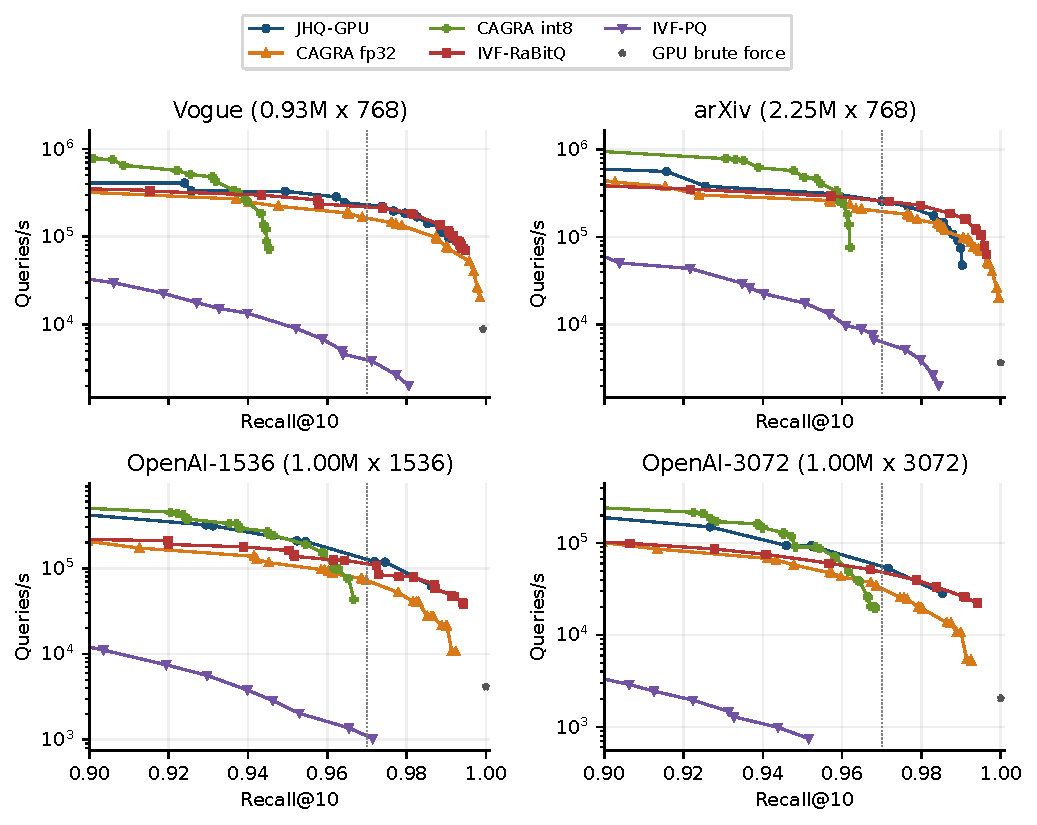
\includegraphics[width=\linewidth]{ch7/frontiers.pdf}
\caption{四个 E1 数据集上实测的主机到主机召回率—QPS 前沿。图中从召回率 0.90 开始显示，并在 0.97 处标出竖线；构造前沿时纳入了包括 CAGRA int8 在内的全部基线组。连线连接实测点，吞吐量轴为对数坐标。}
\label{fig:7-frontiers}
\end{figure}

这些曲线比较的是可达到的吞吐量，而不是相同显存占用下的表现。JHQ 每个向量约存储 $d/8$ 字节主码、$d$ 字节残差码以及元数据。九比特 RaBitQ 的名义编码预算为 $9d/8$ 字节，与 JHQ 接近，但它的 4/8-bit 配置使用更少存储。CAGRA int8 还存储图边；PQ 编码长度可变；CAGRA fp32 保留 FP32 向量。对这些选项取性能包络有助于部署选择，但不能单独证明相同显存预算下的表示优势。显存证据在\cref{sec:7-7}另行讨论。

\subsection{匹配召回率与不同运行区间的反向结果}

\Cref{tab:7-matched} 使用两种估计方式，量化召回率 0.97 附近的表现。插值估计在相邻前沿点之间对吞吐量取对数后进行线性插值，不向覆盖范围之外外推。实测阈值估计选取达到目标召回率的最快采样点。插值估计将与目标相差不超过 $5\times10^{-4}$ 的实测召回率视为匹配；实测阈值估计则要求召回率至少达到目标。插值减小了参数网格间距不一致的影响；实测阈值估计对应真实记录过的配置。两者都不能凭空产生一个召回率恰好等于目标的新测量。

\begin{table}[tbp]
\centering
\caption{召回率 0.97 下的比较。每组比值依次为“插值 / 实测阈值”；大于一表示 JHQ 更快。JHQ kQPS 为插值估计。arXiv 与 RaBitQ 的微小差异随估计方法而改变方向。}
\label{tab:7-matched}
\small\setlength{\tabcolsep}{4pt}
% Generated by scripts/build_zh_tables.py; numeric rows reuse English tables.
\begin{tabular}{@{}lrrr@{}}
\toprule
数据集 & JHQ kQPS & 相对 CAGRA fp32 & 相对 IVF-RaBitQ \\
\midrule
Vogue & 230.8 & 1.416 / 1.537 & 1.059 / 1.046 \\
arXiv & 258.6 & 1.317 / 1.422 & 0.996 / 1.015 \\
OpenAI-1536 & 126.7 & 1.747 / 2.294 & 1.130 / 1.111 \\
OpenAI-3072 & 55.9 & 1.747 / 2.088 & 1.157 / 1.346 \\
\bottomrule
\end{tabular}

\end{table}

相较于 CAGRA fp32，该目标下的插值比值从 arXiv 的 $1.317\times$ 到两个 OpenAI 数据集的 $1.747\times$ 不等。相较于 IVF-RaBitQ，对应数值分别为 $1.059\times$、$0.996\times$、$1.130\times$ 和 $1.157\times$。arXiv 的结果应视为接近平手：插值吞吐量略低，但实测阈值比较略高。如果将其表述为明确获胜，就会让插值约定获得超出测量本身所支持的证据权重。

在有共同覆盖的比较中，目标召回率 0.90--0.985 范围内，JHQ 相对 CAGRA fp32 的插值优势约为 $1.10$--$2.44\times$。但是，加入 CAGRA int8 后，低召回率区间的解释发生变化：在 0.90--0.92 附近，其低精度图搜索可以快于 JHQ。在更高召回率下，IVF-RaBitQ 常重新领先，包括若干 0.98 及以上目标。在 arXiv 约 0.99 的召回率处，记录网格中的 CAGRA fp32 也快于 JHQ。因此，可被证据支持的结论是：JHQ 在部分有价值的区间具有竞争力，尤其是中高召回率附近，而不是全面优于现代 GPU ANN 方法。

CAGRA int8 在 Vogue、arXiv、OpenAI-1536 和 OpenAI-3072 上的最高实测召回率分别为 0.9453、0.9620、0.9667 和 0.9683，因此这些网格中没有达到 0.97 的配置。按相同插值规则，目标召回率 0.90--0.92 处，它约比 JHQ 快 $1.20$--$1.98\times$；在 arXiv 的 0.95 和两个 OpenAI 数据集的 0.94 处也仍然更快。0.97 的结果针对具有测量覆盖的方法，不能推广为低于 0.97 的每个目标均领先。

网格稀疏时，两种估计可能有明显差异。例如，OpenAI-1536 在召回率 0.97 处相对 CAGRA fp32 的比值，插值为 $1.747\times$，而按满足阈值的实测点计算为 $2.294\times$。后一个数值包含了基线下一个超过阈值的测量点所付出的代价，不能将其表述为在完全相同召回率下直接测得的同等幅度优势。配套匹配表保留两种估计，并标明没有覆盖的目标，使读者能够区分真实的运行区间结果与参数采样带来的影响。

\subsection{结果解释与比较限制}

JHQ 将低成本主码筛选与选择性残差访问结合。当只需精排少量已扫描候选时，这为其有竞争力的吞吐量提供了合理解释。后面的内核与预算消融直接检验这一解释的部分环节。仅靠跨系统曲线，不能将收益归因于某个单一组件，因为各方法在路由、表示、预处理、索引构建和软件接口上均有差异。尤其是，数据集维度提高的同时，数据分布与规模也在变化。因此，OpenAI 数据集上更大的比值，并不是“维度提高导致 JHQ 优势扩大”的受控证据。

即便对齐主要计时边界，比较中仍存在限制。JHQ 从 C++ 调用，CAGRA 和 PQ 则通过 Python 绑定调用；即使复用资源，主机端开销仍可能有小幅差异。JHQ 输出回传至可分页主机内存，基线使用页锁定内存。编译目标不同，无关的主机负载也无法完全控制。对于很小的性能差距，这些因素不可忽略。五轮测量描述的是已构建索引上的重复执行，不能估计独立重建索引或换一台机器后的变化。

\section{笛卡尔查找表、打包加载与 lane 协作精排}
\label{sec:7-3}

针对 RQ2，消融区分了保持表示不变的查找表、加载改动与协作式残差评分，并同时测量内核效果和整体应用效果。

\subsection{查找表的精确因子化及其吞吐量影响}

笛卡尔因子化改变的是已表示主码距离的计算方式，而不是重新训练一个量化器。将一个八比特笛卡尔编码拆为两个四比特分量，可把 256 项查找表替换为 $2\times16=32$ 项。对于 FP32 表项，每个对应查找表由 1,024 字节降为 128 字节，即缩小八倍。数学上的评分保持不变，但浮点求值顺序仍可能改变末尾比特。因此，仅凭查找表更小，不能断言完整 ANN 输出逐位一致。

\Cref{fig:7-lut} 比较六个数据集上的笛卡尔查找表分组，探针数为 8/32/128/512、固定 $\alpha=100$，以及 $\glut\in\{1,2,4,8\}$。每个变体有五轮计时；除 Stella 使用 999 条查询外，批大小均为 1,000。在 24 个单元中，两组查找表有 22 个取得最高吞吐量中位数。例外是 arXiv 的 128 探针配置，单组约快 0.23\%；以及 OpenAI-3072 的八探针配置，四组约快 0.84\%。这些小差异更适合视为接近平手。新版统计是 22/24，而不是历史 ADC 论文中的 23/24。

\begin{figure}[tbp]
\centering
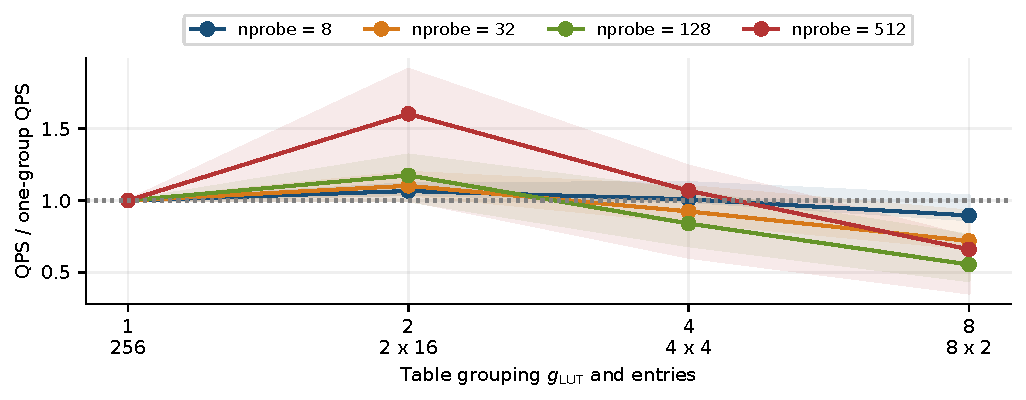
\includegraphics[width=\linewidth]{ch7/lutgroups.pdf}
\caption{固定 $\alpha=100$ 的笛卡尔查找表分组实验（v71）。组数表示 $\glut$，不是并行扫描组数。曲线为各数据集相对单组 QPS 比值的中位数，阴影表示范围。}
\label{fig:7-lut}
\end{figure}

两组相对单组的吞吐量比值为 $0.998$--$1.914$。四组与八组都只需总计 16 个表项，但查表次数和粒度不同。这构成了有用的对照：在两组设计的基础上进一步缩小表存储，并不必然提高搜索性能。额外的索引计算与累加工作可能超过存储节省带来的收益。测量建立的是净收益与开销之间的权衡；缺少独立的占用率或指令计数实验，就不能将某个硬件因素认定为唯一原因。任一四变体单元内，报告的最大召回率差为 $10^{-4}$。

\subsection{打包访存与协作式残差评分}

历史打包实验固定数据集、探针数和查找表分组，比较以字节和机器字为单位的访存。在六个数据集、四个探针数以及 $\glut\in\{1,2\}$ 的 48 对比较中，吞吐量比值为 $1.012$--$1.658$，最大召回率差为 $10^{-4}$。八探针时收益通常较小，512 探针时较大。两种实现都已经采用子空间优先布局，因此，这个实验支持打包访存的效果，而不是“仅靠物理转置就取得了提升”的说法。每个变体只报告一个汇总吞吐率，因而这一较早证据提供的不确定性信息弱于五轮计时的 v71 扫描。

\Cref{fig:7-packing-refinement,tab:7-refinement} 进一步区分了残差精排中更宽加载与 lane 协作的作用。L0 是原始标量路径；L1 改变加载方式，但不将单个候选分给多个 lane；L16 则由 16 个 lane 协作处理一个候选。同一进程在五轮计时中轮换变体顺序，每轮每个变体执行三次搜索。在十二个普通配置上，L16 的端到端吞吐量为 L0 的 $1.015$--$1.789\times$。另外加入的 arXiv $\alpha=200$ 配置明确属于高预算对照，达到 $2.383\times$；不能把它并入普通所选预算的收益范围。

\begin{figure}[tbp]
\centering
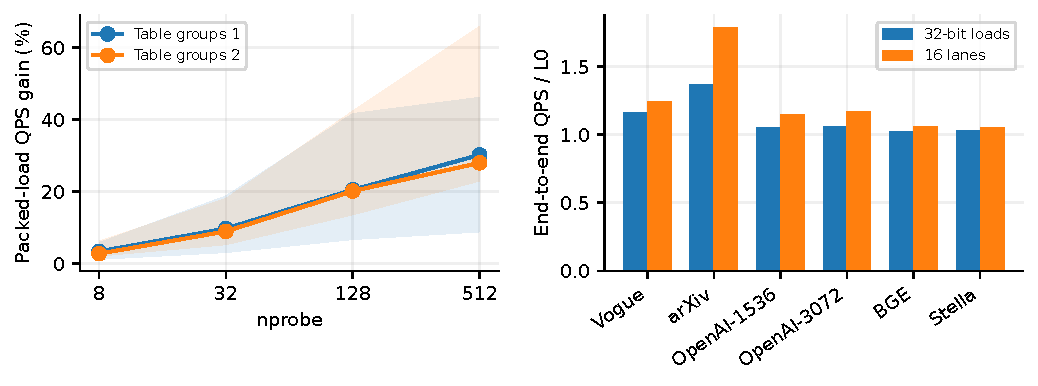
\includegraphics[width=\linewidth]{ch7/packing_refinement.pdf}
\caption{打包访存与精排对照。左：各查找表分组和探针数下，六个数据集打包加载 QPS 增益的中位数，阴影为最小值至最大值。右：128 探针及各数据集普通预算下，仅改变加载和使用 16 个 lane 的实测端到端收益。两个子图来自不同实验组。}
\label{fig:7-packing-refinement}
\end{figure}

\begin{table}[tbp]
\centering
\caption{128 探针下的精排结果。除最后一列为剖析得到的精排内核加速比外，其余比值均为相对 L0 的配对端到端收益。不能将内核加速比与应用整体加速比混用。}
\label{tab:7-refinement}
\small\setlength{\tabcolsep}{4pt}
% Generated by scripts/build_zh_tables.py; numeric rows reuse English tables.
\begin{tabular}{@{}lrrrr@{}}
\toprule
数据集 & $\alpha$ & L1/L0 吞吐比 & L16/L0 吞吐比 & 内核加速比 \\
\midrule
arXiv & 100 & 1.368 & 1.789 & 5.97 \\
BGE & 32 & 1.026 & 1.062 & 1.97 \\
OpenAI-1536 & 8 & 1.055 & 1.145 & 3.34 \\
OpenAI-3072 & 4 & 1.063 & 1.171 & 8.81 \\
Stella & 16 & 1.030 & 1.053 & 2.66 \\
Vogue & 64 & 1.161 & 1.240 & 3.72 \\
\bottomrule
\end{tabular}

\end{table}

在被测用例中，仅改变加载的对照与 L0 逐位一致，但已使 arXiv 吞吐量提高至 $1.368\times$。lane 协作进一步缩短了精排时间。在 arXiv 的 $\alpha=100$ 配置上，精排内核由 4,277.5 降至 716.8\,$\mu$s，即 $5.97\times$ 的内核加速，但整体吞吐量只提高至 $1.789\times$。OpenAI-3072 的精排内核加速为 $8.81\times$，整体吞吐量则为 $1.171\times$。这与 Amdahl 定律一致：加速一个较小阶段，并不能消除路由、筛选、最终选择或传输的成本。这也说明了随后扫描与探针实验的动机——继续处理剩余工作。

定量 Amdahl 检验使用基线精排内核时间占主机到主机基线延迟的比例 $f$，以及内核加速比 $s$；若其余耗时不变，整体估计为 $1/(1-f+f/s)$。arXiv 和 OpenAI-3072 的比例约为 0.529 和 0.168，对应估计 $1.787\times$ 和 $1.175\times$，接近实测 $1.789\times$ 和 $1.171\times$。它结合了单独的内核剖析与墙钟测量，只是机制解释的估计。

协作归约改变了浮点加法顺序。被测多 lane 变体的距离差异很小，最大报告相对误差约为 $1.6\times10^{-6}$，但排序边界附近偶有结果变化。因此，证据支持的是数值接近、且具有实测端到端收益的评分，而不是无条件的逐位等价。Sanitizer 检查在较小查询子集上覆盖了记录中的精排和 top-$k$ 内核；这些是有用的实现检查，并不是对任意输入的证明。

\section{全局 top-c、共享界与探针选择的正确性及消融}
\label{sec:7-4}

本节先回答 RQ2 的正确性部分，再考察分组扫描、阈值共享和基数探针选择的成本。

\subsection{先验证全局主码选择，再讨论性能}

并行扫描实验处理了一个仅靠召回率无法评估的正确性要求：将同一查询的候选分配给多个线程块后，必须保持全局主码 top-$c$。如果每块只保留 $c/\gscan$ 个候选，候选质量集中的分组可能丢弃本应进入全局结果的候选。JHQ 的分组扫描路径改为每组最多保留 $c$ 个候选，再合并局部列表。选择使用完整排序键 $(\primarydist,\mathrm{position})$，以位置确定性地打破主码距离并列。

局部保留规则有直接的正确性解释。一个属于全局 top-$c$ 的候选，在整个候选集合中排在它之前的键少于 $c$ 个，那么在自身所在分组中也一定少于 $c$ 个。因此，它必然出现在该组的局部 top-$c$ 中。对这些局部列表的并集使用相同全序选取 top-$c$，即可恢复全局 top-$c$。这一结论仅针对已访问候选上的主码评分；它不会使 IVF 路由变成精确搜索，不会将主码评分变成原始向量距离，也不会使最终 ANN 答案成为精确最近邻结果。

分组扫描检查覆盖四个工作负载、批大小 8/32/256/1,000，以及分组数 1/2/4/8，共计 64 个比较。记录显示，相对原始单线程块路径，没有非并列情况下的主码选择差异，所比较主码距离的变化为零，而且每条实际使用查询的最终 top-10 标识符与距离逐位一致。原始路径只按距离排序，因此在主码截断边界发生并列时，可能选中不同成员；这并不违反新完整键的规范。在这一特定实验中，这些差异也未改变最终输出。

实际使用的查询数需要单独说明。测试程序只提交完整批次：从 1,000 条查询池中，批大小 32 使用 992 条，批大小 256 使用 768 条，而批大小 8 和 1,000 均使用全部 1,000 条。因此，正确性计数与计时样本随批大小而变化，不能把每一行都描述为相同的 1,000 查询测试。记录中的 memcheck、racecheck 和 synccheck 还对更小子集及指定扫描、合并内核提供了额外检查。

\subsection{共享界保持选择目标不变}

保留完整局部 top-$c$ 是安全的，但成本可能很高。在共享界组件（v63）中，同一查询的各组通过相同完整排序键发布共享界。一旦某组已确定有 $c$ 个键不大于该界，比该界更差的候选就不可能进入全局 top-$c$。过时、较宽松的界可能接纳更多候选，但不会因此错误地排除更优候选。这要求发布的界有足够数量的有效候选作为依据，并且原子更新保持完整键的顺序；仅有近似距离阈值，无法建立相同的并列处理语义。

实现仍会先为每个扫描候选计算完整主码评分，再决定是否接纳。共享界减少的是选择、压缩整理、排序与后续合并工作；它不会剪去主码距离计算，也不会避免读取所有被拒绝候选的主码。解释扫描阶段加速时，必须明确这一范围：扫描阶段变快，并不一定意味着计算了更少距离。

共享界检查，在四个工作负载与四种批大小上，将共享界的 2/4/8 组路径与相应独立界路径比较。48 个比较全部报告主码 top-$c$ 和最终输出一致。五轮配对吞吐量相对独立界约为 $0.994$--$1.562\times$。因此，共享界能显著帮助部分高成本配置，但并非处处更快。在 arXiv 的 $\alpha=200$、批大小 1,000、八组配置上，同一次配对剖析中，合并成本约由 2,629 降至 471\,$\mu$s，扫描则由 7,968 降至 5,513\,$\mu$s。结果支持减少过量中间工作，而不是“扫描分组越多越好”。

另一种未采用的方案是分配更小的静态局部配额。先导工作负载的分布测量显示，第一候选组包含 46--81\% 的全局保留候选。等额配额会经常需要正确性回退；即使校准不等额配额，主导分组仍处于关键路径。这些观测促成了精确共享界设计，但它们只是这些工作负载上的先导测量，不能证明所有可能的配额策略都更差。

\subsection{精确探针选择与流水线一致性的边界}

当筛选变快后，IVF 探针选择在小批次时间中的占比会提高。基数探针原语（v69）改变了选取最小质心评分的实现，同时保留 FP32 评分。其合成检查覆盖 1,792 个用例，失败数为零。在真实 arXiv、Vogue 和 OpenAI-3072 工作负载上，检查发现全部 1,000 条查询的探针标识符相同，主码 top-$c$ 位置与距离也相同。这比“召回率数字没有变化”更具体，因为它直接检查了路由和筛选输出。

\begin{table}[tbp]
\centering
\caption{精确 FP32 探针选择改动的 v69/v65 端到端吞吐量比。每个工作负载—批大小比较中，每个二进制程序共计时十轮，采用交替运行。大于一表示 v69 更快。}
\label{tab:7-probe}
\small
% Generated by scripts/build_zh_tables.py; numeric rows reuse English tables.
\begin{tabular}{@{}lrrrr@{}}
\toprule
数据集 & 批大小 8 & 32 & 256 & 1,000 \\
\midrule
arXiv & 1.074 & 1.063 & 1.035 & 1.034 \\
Vogue & 1.109 & 1.103 & 1.052 & 1.041 \\
OpenAI-3072 & 1.167 & 1.117 & 1.055 & 1.050 \\
\bottomrule
\end{tabular}

\end{table}

\Cref{tab:7-probe} 显示端到端吞吐量提高至 $1.034$--$1.167\times$。批大小为 8 时，剖析得到的探针阶段在 arXiv 上从 56.5 降至 22.6\,$\mu$s，在 Vogue 上从 52.7 降至 14.7\,$\mu$s，在 OpenAI-3072 上从 77.8 降至 16.7\,$\mu$s。大批次下，未修改阶段占整体耗时比例更高，因此整体收益较小符合预期。这些是各自实验组内部的比值，不能把它们与前面的 v62 或精排收益相乘，仿佛所有测量都共享同一个基线。

Vogue 区分了探针原语与跨进程流水线可复现性。在一组、批大小 8 的测试中，两种二进制的探针/主码 dump 对全部 1,000 条查询逐字节相同，但最终召回率为 0.9642 与 0.9644。同一个基线二进制也从一致性运行中的 0.9642，变成之后两次计时运行中的 0.9644。因此，观察到的变化并不需要探针改动才能发生；在 dump 控制的用例中，它出现在已记录主码选择边界之后。残差表示、输入和评分计算仍是可能来源，根因尚未确定。在各被检进程内部，调度与单线程块输出仍逐位一致。附录~\ref{app:reproducibility}明确了 dump 的覆盖范围，避免将其当作对每条计时路径的检查。

最后，可选的 v70 FP16 实验属于另一项近似。在 arXiv 的 936/1,000 条、Vogue 的 979/1,000 条、OpenAI-3072 的 998/1,000 条查询上，其探针集合与 FP32 完全相同，平均集合重叠率很高。但高重叠率和很小的召回率变化，并不能使该原语变成精确操作。这些结果不纳入主要 E1 前沿，也不纳入精确探针选择结论。

\section{留出查询上的预算质量、吞吐量与回本}
\label{sec:7-5}

RQ3 考察相对可信固定预算的质量和摊销成本。因此，比较同时包含沿用的 $\alpha=100$ 与更强的统一固定对照 $\alpha=64$。

\subsection{无标签选择与使用标签的诊断性 oracle}

预算实验在每个数据集—探针数组合中固定一个训练好的索引，比较固定预算、抽样校准、全校准池校准、同样本枚举与离线 oracle。六个数据集均测试 128 和 512 探针。偶数下标查询组成 500 条校准池；奇数下标查询组成互不重叠的 500 条留出池，Stella 例外，留出池为 499 条。从校准池中使用固定随机种子抽取 $S\in\{32,64,128\}$ 条查询，每种大小重复抽取 64 次；单次抽样内不放回。重复抽样使用的是同一个有限查询池，并不等于对未来工作负载漂移进行 64 次独立采样。

降序预算网格为 $A=(200,100,64,32,16,8,4,2)$。校准将候选预算的 top-10 标识符集合与 $\alpha_{\max}=200$ 的参考结果比较。对于样本 $\mathcal Q_S$，接受统计量为
\begin{equation}
 D_S(\alpha)=\sum_{q\in\mathcal Q_S}
 \left(10-|\mathcal R_\alpha(q)\cap\mathcal R_{200}(q)|\right),
 \qquad D_S(\alpha)\leq 1.
 \label{eq:7-agreement}
\end{equation}
允许的是整个样本合计一个结果槽位不一致，而不是每条查询允许一个，也不是基于 ground truth 的召回率容差。实际规则不接收标签。参考结果本身也是近似结果，因此完全一致也可能复制其错误。

离线 oracle 的作用不同。它查看八个固定预算在留出池上的召回率后，在距最佳实测留出召回率不超过 $10^{-3}$ 的配置中选择最快者。这是诊断性比较标准，不是可直接部署的无标签决策。“全校准池”同样表示在全部 500 条校准查询上应用同一校准搜索，而不是利用留出标签枚举所有预算。这些区分避免将“选到与 oracle 相同预算”误解为质量保证。

\subsection{预算质量与抽样风险}

\Cref{tab:7-budget-quality} 给出了 $S=128$ 的结果。十二个单元中，所选预算的中位数有十个与 oracle 预算一致；不一致的两个是 arXiv 的 128 探针配置和 OpenAI-3072 的 512 探针配置。所选预算跨越 4--200，显示出明显的工作负载依赖。然而，预算中位数与平均召回率描述的是抽样总体的不同方面，二者不一定对应某一个配置的性能。此外，表中平均召回率由日志打印的最佳召回率减去打印的平均损失重构，所以保留到四位小数的值是近似值。

\begin{table}[tbp]
\centering
\caption{$S=128$ 时的留出质量。规则的 $\alpha$ 是 64 次抽样的中位数，oracle 的 $\alpha$ 使用留出标签。$\overline R_{\rm rule}$ 是重构的平均召回率。“超标”统计相对最佳被测留出召回率损失 $>10^{-3}$ 的抽样次数；$L_{95}$ 是日志采用较低次序统计量得到的 95 分位损失估计。$R_{100}$ 是固定预算召回率。}
\label{tab:7-budget-quality}
\small\setlength{\tabcolsep}{3pt}
% Generated by scripts/build_zh_tables.py; numeric rows reuse English tables.
\begin{tabular}{@{}lrrrrrr@{}}
\toprule
数据集 & 探针数 & $\alpha$：规则/oracle & $R_{100}$ & $\overline{R}_{\rm rule}$ & 超标 & $L_{95}$ \\
\midrule
Vogue & 128 & 64 / 64 & 0.9680 & 0.9677 & 5/64 & 0.0022 \\
arXiv & 128 & 100 / 200 & 0.9748 & 0.9751 & 40/64 & 0.0024 \\
OpenAI-1536 & 128 & 8 / 8 & 0.9280 & 0.9279 & 4/64 & 0.0000 \\
OpenAI-3072 & 128 & 4 / 4 & 0.9252 & 0.9252 & 0/64 & 0.0000 \\
BGE & 128 & 32 / 32 & 0.9198 & 0.9190 & 1/64 & 0.0008 \\
Stella & 128 & 16 / 16 & 0.9892 & 0.9884 & 6/64 & 0.0030 \\
Vogue & 512 & 64 / 64 & 0.9916 & 0.9915 & 2/64 & 0.0002 \\
arXiv & 512 & 200 / 200 & 0.9878 & 0.9885 & 32/64 & 0.0016 \\
OpenAI-1536 & 512 & 8 / 8 & 0.9740 & 0.9738 & 4/64 & 0.0000 \\
OpenAI-3072 & 512 & 4 / 8 & 0.9704 & 0.9702 & 0/64 & 0.0002 \\
BGE & 512 & 64 / 64 & 0.9670 & 0.9661 & 24/64 & 0.0014 \\
Stella & 512 & 16 / 16 & 0.9954 & 0.9945 & 7/64 & 0.0030 \\
\bottomrule
\end{tabular}

\end{table}

一个重要反例是 arXiv。在 128 探针下，即使平均损失仅为 0.0009，仍有 40/64 次抽样的召回率损失超过 $10^{-3}$；512 探针下有 32/64 次超标。BGE 的 512 探针配置有 24/64 次超标，95 分位损失为 0.0014。Stella 超标次数较少，但两个探针数下的 95 分位损失均为 0.0030。因此，平均质量、超标频率与尾部损失幅度必须一起看。OpenAI-3072 在这些抽样中未观察到超标，这支持其在当前查询池上的有利表现，却不是对未见查询的零风险保证。

对于数量较少的抽样，分位数约定也很重要。测试程序报告排序损失中从零起算的 $\lfloor0.95(64-1)\rfloor=59$ 项，而不是在次序统计量之间插值。因此，可能同时存在四个非零尾部损失，而打印的 $L_{95}=0$，OpenAI-1536 就是如此。表格保留日志统计量与准确超标次数；该列为零不等于所有抽样都没有损失。

\begin{figure}[tbp]
\centering
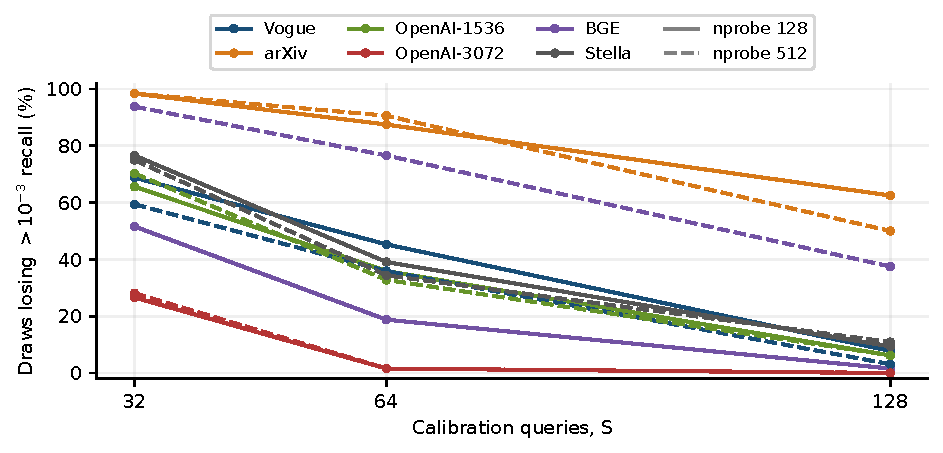
\includegraphics[width=0.82\linewidth]{ch7/budget_risk.pdf}
\caption{不同样本大小下的留出风险。纵轴为相对最佳被测预算，留出召回率损失超过 $10^{-3}$ 的校准抽样百分比。由于\cref{eq:7-agreement}始终保持阈值一，增加 $S$ 也收紧了允许的槽位不一致比例。}
\label{fig:7-budget-risk}
\end{figure}

\Cref{fig:7-budget-risk} 显示了样本大小的影响。更大的样本通常使选择更保守，但同时收紧了归一化允许量 $1/(10S)$。在全部 2,304 次抽样（$12\times3\times64$）中，同样本枚举与二分搜索一致，而打印日志显示枚举耗时为其 1.75--2.01 倍。

被测默认路径执行精确主码 top-$c$，最终 top-$k$ 遍历全部 $c$ 个精排候选，并按 ID 打破并列。有损的 \texttt{K\_LOCAL=4} 保留路径是设置 \texttt{JHQ\_EXACT\_TOPCK=0} 才启用的替代路径，并不是本预算实验单调性限制的原因。在评分固定、采用共同全序并列规则时，精确主码选择得到嵌套候选集，因此抽样一致性准则满足单调性。剩余限制是一块路径在截断并列处只比较距离，以及批大小会决定使用单线程块还是按完整键排序的分组扫描。因此，小校准批次和留出查询批次可能采用不同执行路径。枚举一致验证了这个网格上的抽样决策，并不保证留出召回率，也不保证跨路径无条件嵌套。

固定预算也并不完美。\Cref{tab:7-fixed-budget} 按诊断性质量目标评估了全部八个固定选项。固定 $\alpha=100$ 在十二个单元中有十个达标；$\alpha=200$ 全部达标，但可能牺牲较多吞吐量。全校准池校准也不等于 oracle：在 Vogue 两个探针数下，它均选择 100，而 oracle 选择 64。即使增加校准样本，基于输出一致性的选择与“质量约束下最快”的选择仍解决不同问题。全校准池耗时为 9.5--60.3\,ms。在这十二个单元中，$\alpha=200$ 达到最高实测召回率，因此作为高预算覆盖对照；12/12 达标不是独立的质量保证。网格中的吞吐量也并非严格单调：例如，OpenAI-3072 在 128 探针下，$\alpha=2$ 为 128.7 kQPS，$\alpha=4$ 为 145.0 kQPS。三次计时无法区分时间波动与配置相关执行成本，所以本章不为该倒置认定机制。

\begin{table}[tbp]
\centering
\caption{十二个留出单元上的固定预算对照。达标表示按打印精度，距最佳被测召回率不超过 $10^{-3}$。最大召回率损失使用全部单元，QPS 差额只统计该预算达标的单元。横线表示没有达标单元。}
\label{tab:7-fixed-budget}
\small
% Generated by scripts/build_zh_tables.py; numeric rows reuse English tables.
\begin{tabular}{@{}rrrr@{}}
\toprule
$\alpha$ & 达标单元 & 最大召回率损失 & 达标单元最大 QPS 差额 \\
\midrule
2 & 0/12 & 0.3100 & -- \\
4 & 2/12 & 0.1774 & 2.3\% \\
8 & 4/12 & 0.0930 & 2.1\% \\
16 & 6/12 & 0.0408 & 4.4\% \\
32 & 7/12 & 0.0170 & 9.1\% \\
64 & 10/12 & 0.0050 & 26.6\% \\
100 & 10/12 & 0.0016 & 40.9\% \\
200 & 12/12 & 0.0000 & 57.1\% \\
\bottomrule
\end{tabular}

\end{table}

\subsection{估计吞吐量与校准经济性}

与 E1 不同，这组实验在预热后，对每个固定配置进行三次搜索计时。规则报告的 QPS 是 64 次抽样所选配置的已有实测 QPS 的算术平均，而不是对一个重复执行“校准—搜索”的服务进行新计时。当 $S=128$ 时，这一所选配置吞吐量估计在十个单元中优于固定 $\alpha=100$，比值为 $1.028$--$1.691\times$。arXiv 的比值则为 0.908 和 0.917：平均召回率提高，但吞吐量降低。这两个单元无法通过吞吐量收益回本。

更强的 $\alpha=64$ 对照缩小了整体收益：所选配置的平均 QPS 在 9/12 个单元中胜出，几何平均比值为 $1.054\times$，范围为 $0.821$--$1.367\times$。Vogue 几乎不变；BGE 的 512 探针配置只提高 0.6\%；OpenAI 的收益范围为 $1.052$--$1.367\times$。固定 64 和固定 100 都在 10/12 个单元达标，失败的都是两个 arXiv 单元。校准的价值是适应不同精排需求，而不是始终击败已经合理的固定预算。

arXiv 的超标是相对最佳被测留出召回率，不是相对默认配置。固定 100 在 128 和 512 探针下本来分别损失 0.0012 和 0.0016，而抽样平均损失在两个单元均为 0.0009。因此，即使部分抽样超过相对 oracle 的目标，平均质量仍比默认配置更好。

\begin{table}[tbp]
\centering
\caption{校准经济性，$S=128$。速率单位为 kQPS，规则速率为所选配置平均 QPS。比值分别相对固定 100 与固定 64。最后一列回本相对固定 100，使用 500 条查询，Stella 为 499；“不回本”表示没有吞吐量回本。}
\label{tab:7-budget-cost}
\footnotesize\setlength{\tabcolsep}{3pt}
% Generated by scripts/build_zh_tables.py; numeric rows reuse English tables.
\begin{tabular}{@{}lrrrrrrrr@{}}
\toprule
数据集 & 探针数 & $Q_{100}$ & $\overline Q_{\rm rule}$ & 相对 100 & 相对 64 & 校准 ms & 回本批数 & \shortstack{固定 100\\质量} \\
\midrule
Vogue & 128 & 202.9 & 224.4 & 1.106 & 1.004 & 4.0 & 17.0 & 达标 \\
arXiv & 128 & 207.9 & 188.8 & 0.908 & 0.821 & 4.2 & 不回本 & 未达标 \\
OpenAI-1536 & 128 & 167.5 & 268.5 & 1.603 & 1.367 & 3.9 & 3.5 & 达标 \\
OpenAI-3072 & 128 & 85.7 & 145.0 & 1.691 & 1.230 & 5.7 & 2.4 & 达标 \\
BGE & 128 & 116.2 & 131.2 & 1.130 & 1.051 & 6.5 & 13.2 & 达标 \\
Stella & 128 & 95.7 & 110.3 & 1.153 & 1.087 & 7.5 & 10.8 & 达标 \\
Vogue & 512 & 100.1 & 102.9 & 1.028 & 0.996 & 7.5 & 55.4 & 达标 \\
arXiv & 512 & 83.1 & 76.2 & 0.917 & 0.870 & 9.7 & 不回本 & 未达标 \\
OpenAI-1536 & 512 & 86.6 & 115.0 & 1.327 & 1.268 & 8.8 & 6.2 & 达标 \\
OpenAI-3072 & 512 & 42.8 & 52.1 & 1.219 & 1.052 & 13.1 & 6.2 & 达标 \\
BGE & 512 & 49.2 & 51.1 & 1.039 & 1.006 & 15.8 & 41.2 & 达标 \\
Stella & 512 & 34.6 & 36.0 & 1.041 & 1.028 & 21.3 & 37.1 & 达标 \\
\bottomrule
\end{tabular}

\end{table}

日志中的校准成本为 3.9--21.3\,ms。它包含参考搜索与输出一致性检查，以及测量搜索调用内包含的相关设置，但不包含将抽样向量收集到输入缓冲区的操作。对于相同大小的后续批次，定义
\begin{equation}
 B^*=\frac{T_{\rm cal}}{T_{100}-T_{\rm rule}},\qquad
 T_{\rm rule}<T_{100}.
 \label{eq:7-payback}
\end{equation}
使用 $T_{\rm rule}\approx n/\overline Q_{\rm rule}$ 得到\cref{tab:7-budget-cost}中的估计：有利单元相对固定 100 约需 2.4--55.4 个留出池大小的后续批次。相对固定 64，九个有利单元约需 5.7--404.3 批，Vogue 的 512 探针配置没有吞吐量回本。\Cref{fig:7-budget-payback}对两个对照都使用实际留出查询数。

\begin{figure}[tbp]
\centering
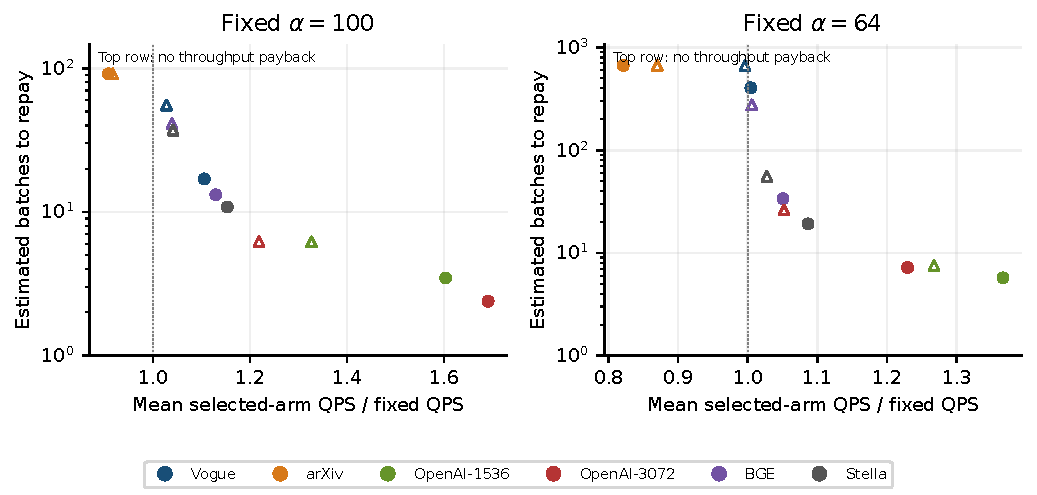
\includegraphics[width=\linewidth]{ch7/budget_payback.pdf}
\caption{相对固定预算 100 和 64 的校准回本估计。实心圆表示 128 探针，空心三角表示 512 探针；顶行点没有吞吐量回本。估计对所选配置平均 QPS 取倒数，使用 500 条查询，Stella 为 499。}
\label{fig:7-budget-payback}
\end{figure}

这种计算偏乐观。一般而言，$1/\mathbb E[Q]\leq\mathbb E[1/Q]$，所以当不同校准抽样选择了速率不同的配置时，对平均 QPS 取倒数会低估平均执行时间。样本收集、未来查询漂移与重新校准开销也会影响摊销。对于长期稳定的工作负载，复用策略可能带来收益；短任务或变化的查询总体则未必如此。当前实验没有测量漂移检测，也没有测量生产环境中的重新校准计划。

作为历史比较，较早的标量精排实现（v57）在 10/12 个单元中报告相对固定 100 的 $1.054$--$2.773\times$ 收益，校准耗时为 5.2--30.8\,ms。较新的 lane 精排流水线收益更小，与可节省精排时间减少的解释相容。两次运行共享预算协议和网格，但跨实验比较并未隔离证明精排是变化的唯一原因。

\section{批大小、扫描组调度与工作负载偏斜}
\label{sec:7-6}

本节回答 RQ2 的性能区间问题：何时额外扫描组提供有价值的并行度，何时额外工作成为主导。

\subsection{并行度与重复选择工作的权衡}

扫描实验揭示了两种执行区间。每条查询使用一个线程块时，批大小 8 只在具有 170 个 SM 的设备上提供八个线程块。划分候选能增加可用线程块并行度。在 v62 实验中，批大小 8 使用八组后，端到端吞吐量为原来的 $2.06$--$2.76\times$。剖析给出了阶段解释：arXiv 扫描约从 849 降至 216\,$\mu$s，Vogue 从 1,059 降至 246\,$\mu$s，OpenAI-3072 从 728 降至 155\,$\mu$s。额外合并分别约需 16.7、9.1 和 3.7\,$\mu$s。即使支付合并成本，净节省仍很大。

批大小为 1,000 时，独立查询已足以提供较多线程块。增加分组会重复搬入查找表、接纳局部候选并排序，还产生额外合并流量。对于 arXiv 的 $\alpha=200$ 配置，不共享界的 v62 路径可能降至单线程块基线的约 $0.46\times$。全批次剖析显示，$\alpha=100$ 的扫描从 2,922 增至 6,079\,$\mu$s，$\alpha=200$ 从 3,530 增至 7,652\,$\mu$s，后者还增加了 2,624\,$\mu$s 合并时间。这一反向结果对设计至关重要：并行拆分能够解决并发不足，但当并发已经充足时，它引入的额外工作可能成为主导。共享界减少了这些额外工作，却没有消除执行区间的变化。

\begin{figure}[tbp]
\centering
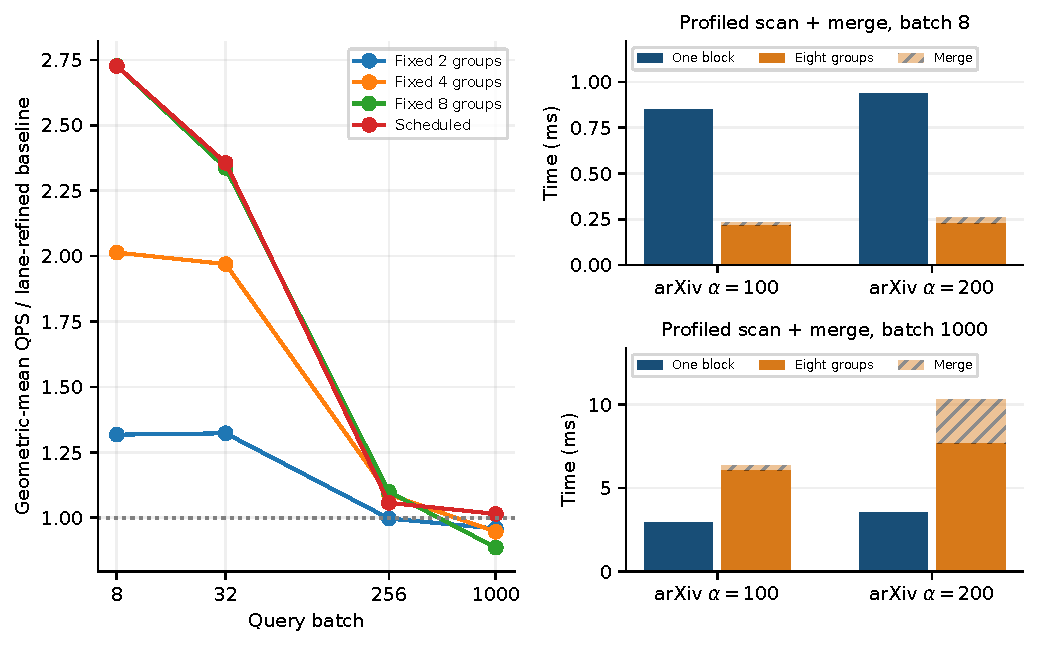
\includegraphics[width=\linewidth]{ch7/batch_execution.pdf}
\caption{执行区间。左：共享界固定组数与调度执行，相对 lane 精排单线程块基线的吞吐量比，较小批次有 13 个单元，批大小 1,000 有 11 个。右：arXiv 预算 100 和 200 在批大小 8 与 1,000 下的配对扫描、合并剖析；斜线表示合并时间。右侧来自独立界扫描实验，用于解释一项成本，不代表调度器全部收益。}
\label{fig:7-batch}
\end{figure}

\subsection{在更多配置上评估预先固定的规则}

集成批调度器（v65）根据批大小、线程块大小以及工作负载偏斜估计选择扫描组数。填充规则将潜在线程常驻数量与设备线程容量的固定 0.6 比例关联；偏斜规则则在每条查询候选数的变异系数至少为 0.3 时，要求至少使用四组。最终取两条规则建议的较大组数；一组情况映射到原始单线程块扫描。偏斜统计只估计一次，使用 512 个数据库向量作为伪查询，不使用 ground-truth 标签或被测查询池。规则常数在四个工作负载配置上确定，之后才测量额外配置。

\begin{table}[tbp]
\centering
\caption{集成执行相对 v61 L16 的收益。每项先计算单元内五轮配对加速比的中位数，再跨单元取几何平均。“留出配置”排除了设置规则时使用的四个配置，指的是未用于设定规则的配置，不是预算实验中的留出查询划分。}
\label{tab:7-scheduling}
\small\setlength{\tabcolsep}{4pt}
% Generated by scripts/build_zh_tables.py; numeric rows reuse English tables.
\begin{tabular}{@{}rrrrrrr@{}}
\toprule
批大小 & 单元数 & $g_s=2$ & $g_s=4$ & $g_s=8$ & 调度 & 留出配置 \\
\midrule
8 & 13 & 1.318 & 2.014 & 2.728 & 2.727 & 2.930 \\
32 & 13 & 1.323 & 1.970 & 2.337 & 2.356 & 2.560 \\
256 & 13 & 0.997 & 1.090 & 1.099 & 1.057 & 1.041 \\
1000 & 11 & 0.959 & 0.947 & 0.886 & 1.015 & 1.012 \\
\bottomrule
\end{tabular}

\end{table}

\Cref{tab:7-scheduling} 从原始计时数组重新计算结果。批大小为 8、32、256 和 1,000 时，调度收益的几何平均分别为 $2.727\times$、$2.356\times$、$1.057\times$ 和 $1.015\times$。前三种批大小有十三个配置，其中包含额外的 arXiv 高预算配置；批大小 1,000 只有十一个，因为 Stella 的 999 条查询池无法组成一个完整的 1,000 查询批次。对应的留出配置子集分别含九个和七个配置。因此，将这些均值连接起来的图总结的是运行区间，而不是完全平衡的重复测量总体。

固定八组在批大小 8 时的均值接近调度结果，但在批大小 1,000 时降至 $0.886\times$。调度大体保留了小批次收益，并避免上述大批次损失。不过，它仍是启发式规则，不是 oracle。批大小 256 时，在一个 BGE 配置上，“最佳固定吞吐量 / 调度吞吐量”的最差比值为 1.217。候选数 CV 无法描述列表遍历、选择或合并的全部成本。这一失败表明所选特征存在局限，并不说明执行调度没有必要。

Vogue 说明仅看批大小是不够的。其候选数 CV 实测约为 0.51，而原始其他工作负载约为 0.08--0.11；其最重查询的候选数约为均值的 2.2 倍。划分候选能缩短慢查询，而该查询原本可能决定整个同步批次的完成时间。这解释了为何 Vogue 在较大批次下仍可能受益于多组执行，不过这些 CV 观测仍属于工作负载证据，并不是对偏斜作用的普遍因果隔离。

最后，正确性检查独立于计时。在 250 个变体/配置比较、234,320 次逐查询比较中，集成实验未发现非并列主码选择差异，也未发现最终标识符集合差异。在并列情况下，最终顺序可能不同，因而不能将整个实验描述为无条件逐位一致。吞吐量结果针对顺序同步提交，不足以建立开放到达过程下的尾延迟表现。

\section{冷构建、常驻显存与已验证规模}
\label{sec:7-7}

通过冷构建、常驻显存与已完成的大数据集搜索评估 RQ1；E1 显存比较也为 RQ4 提供依据。

\subsection{冷构建与生命周期边界}

主要搜索扫描复用了已训练状态缓存。加载该状态并添加向量不属于冷构建。独立日志明确在训练状态缓存为空时训练，然后编码并添加数据库；\cref{tab:7-build-memory}给出这些记录中的训练与添加时间。合计耗时从 OpenAI-1536 的约 1.01\,s 到 Stella 的 10.40\,s。Stella 的训练为 3.74\,s、添加为 6.67\,s，也说明不能仅凭另一个阶段或数据集规模可靠推断某个阶段的成本。

\begin{table}[tbp]
\centering
\caption{JHQ 冷构建与单独测量的常驻显存。训练和添加来自每个数据集的一次已记录冷构建；显存来自 v71 两组、128 探针、$\alpha=100$ 的运行，包含上下文与工作区。“残差占比”表示模型计算的残差码占实测已用总量的比例，而不是每次查询读取的比例。}
\label{tab:7-build-memory}
\small\setlength{\tabcolsep}{3pt}
% Generated by scripts/build_zh_tables.py; numeric rows reuse English tables.
\begin{tabular}{@{}lrrrrrr@{}}
\toprule
数据集 & 训练 s & 添加 s & 合计 s & 已用 GiB & 原始 GiB & 残差占比 \\
\midrule
Vogue & 1.06 & 0.27 & 1.33 & 1.47 & 2.67 & 45.4\% \\
arXiv & 0.59 & 0.52 & 1.10 & 2.58 & 6.45 & 62.5\% \\
OpenAI-1536 & 0.64 & 0.38 & 1.01 & 2.39 & 5.72 & 59.7\% \\
OpenAI-3072 & 1.34 & 0.65 & 1.99 & 4.14 & 11.43 & 69.0\% \\
BGE & 3.75 & 3.67 & 7.42 & 11.93 & 38.50 & 80.7\% \\
Stella & 3.74 & 6.67 & 10.40 & 20.44 & 67.81 & 82.9\% \\
\bottomrule
\end{tabular}

\end{table}

这里的“冷”指已学习索引状态。输入加载器可复用内存映射 FP32 数据；报告的训练加添加区间不包含从存储设备读取原始导出文件。调度器的伪查询校准在添加之后进行，也不计入总量。完整部署生命周期还应考虑数据准备、某些接口未计入的传输、校准、序列化和后续查询时间。这些记录是在明确边界内有价值的构建测量，不是完整端到端数据摄取服务的成本。

比较图同时给出了其他构建配置与这些冷构建记录。每种方法的范围不是等价重复构建的置信区间。训练样本、索引参数与表示不同，而且每个数据集只有一次 JHQ 冷构建记录。对于 RaBitQ，记录中的构建函数与序列化/反序列化分开计时，但基准必须完成该往返后才能搜索。只有将柱形明确标为构建函数时间时，才可以不计这一步；它并不表示直到第一次可用搜索的全部时间。

\begin{figure}[tbp]
\centering
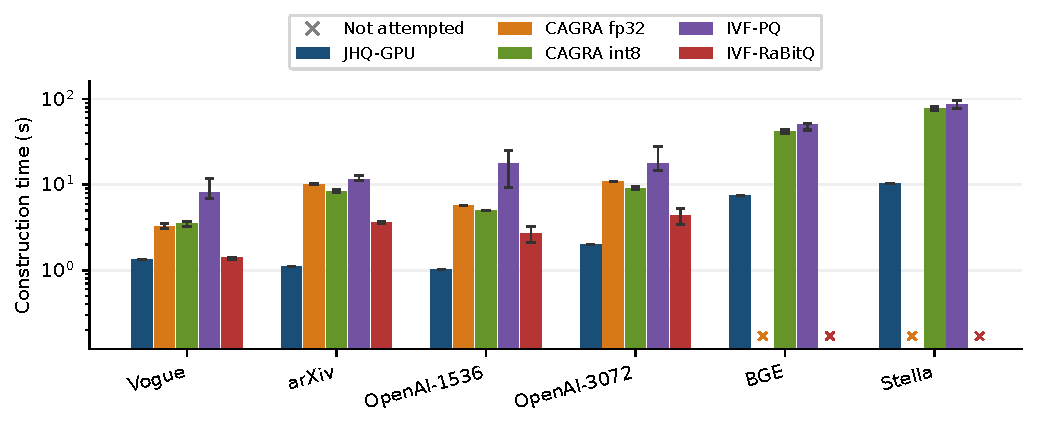
\includegraphics[width=\linewidth]{ch7/construction.pdf}
\caption{包括 CAGRA int8 的已记录构建成本。JHQ 为一次冷训练加添加记录；其他柱形为成功测量的索引配置之间的中位数，误差线表示最小值至最大值。Int8 包含数据集量化；RaBitQ 不包含所需的序列化往返。大数据集缺失的柱形表示未尝试的配置，不代表实测构建失败。纵轴为对数坐标。}
\label{fig:7-build}
\end{figure}

在 Stella 上，CAGRA int8 成功的隔离构建按图出度不同，包含数据集量化后约为 74.55 和 82.45\,s；IVF-PQ 三个配置的实测构建中位数为 86.59\,s。在报告边界内，JHQ 的 10.40\,s 明显更短，但不能据此证明它在所有条件下构建最快，也不能证明后续召回率相同。构建速度、可搜索质量与常驻成本是部署时需要分别考虑的维度。

\subsection{常驻分配与压缩发挥作用的位置}

\Cref{fig:7-memory} 分解常驻显存。标记表示记录时设备已用显存，而不是纯索引分配。堆叠部分用模型计算主码、残差码、修正因子与标识符、质心、每批查找表、候选缓冲区和列表分组临时区。剩余实测分配明确保留为未归因部分；它可能包含运行时上下文、分配器影响以及模型遗漏的分配。将剩余部分全部归给残差码，会高估表示成本。

\begin{figure}[tbp]
\centering
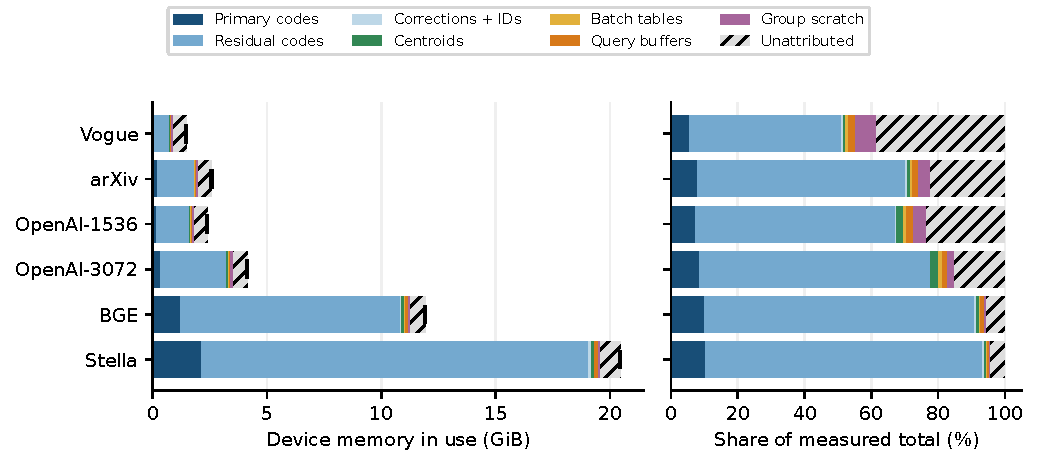
\includegraphics[width=\linewidth]{ch7/memory.pdf}
\caption{两组查找表、128 探针、$\alpha=100$ 下的常驻显存分解。组件大小由模型计算，标记为实测已用总量，斜线区域为未归因部分。总量包含上下文与工作区，未测量构建峰值。}
\label{fig:7-memory}
\end{figure}

在大数据集上，残差码是主要占用：BGE 的已用总量为 11.93\,GiB，其中约 80.7\% 为残差码；Stella 为 20.44\,GiB，其中约 82.9\% 为残差码。仅对应的原始 FP32 向量数组就分别需要 38.50 和 67.81\,GiB。因此，JHQ 通过保留压缩层次表示，使这些已测试的数据能够在单卡常驻搜索。降低 $\alpha$ 会减少每条查询访问、评分的残差码，但不会释放已经存储的残差数组。同样，笛卡尔 LUT 因子化减少的是查询相关查找表存储，不是数据库残差码的精度。

工作区同样重要。在这些 $\alpha=100$ 测量中，报告的列表分组临时区约为 93.8\,MiB，即使实际执行选择单线程块路径，也为批容量 1,024 和最多八组预留。因此，实际组数变小，不意味着分配按比例缩小。另一方面，这些常驻样本没有捕获临时构建峰值。基线测试程序也在测量索引显存之后才初始化部分搜索内存池，因此，不能把构建后的索引增量当作各方法完整进程峰值显存预算。

E1 测量提供了\cref{tab:7-e1-memory}中的独立跨系统视图。从 JHQ 进程总量减去基线测得的 507.2\,MiB 上下文后，约为 CAGRA fp32 索引分配的 0.29--0.39。JHQ 数字包含工作区，CAGRA 数字则是构建时索引增量。这些是参数扫描范围，不是显存匹配的同召回率运行点，也不是相同峰值预算的比较。

\begin{table}[tbp]
\centering
\caption{E1 分配范围。JHQ 为进程总量减去 507.2\,MiB 上下文估计，包含查询工作区；CAGRA fp32 为构建时测量的索引分配。比值范围组合每个数据集的极值。}
\label{tab:7-e1-memory}
\footnotesize\setlength{\tabcolsep}{4pt}
% Generated by scripts/build_zh_tables.py; numeric rows reuse English tables.
\begin{tabular}{@{}lrrr@{}}
\toprule
数据集 & JHQ 净进程 GiB & CAGRA fp32 索引 GiB & 比值范围 \\
\midrule
Vogue & 0.90--1.01 & 2.89--2.91 & 0.31--0.35 \\
arXiv & 2.01--2.19 & 6.84--6.98 & 0.29--0.32 \\
OpenAI-1536 & 1.79--2.33 & 5.95--5.97 & 0.30--0.39 \\
OpenAI-3072 & 3.54--3.82 & 11.67--11.68 & 0.30--0.33 \\
\bottomrule
\end{tabular}

\end{table}

\subsection{大数据集可运行性与竞争区间}

BGE 含 10,091,524 个向量，Stella 含 17,776,615 个向量，均为 1,024 维、32,768 个 IVF 列表。Stella 查询采样自语料库，因此结果描述的是该基准，而不是独立收集的外部查询分布。\Cref{fig:7-large} 包含成功的 CAGRA int8 和 IVF-PQ 测量。对于计算存储需求超过可用设备容量的全精度 CAGRA、RaBitQ 配置和 FP32 暴力搜索，大规模比较没有尝试运行。这些缺项是预先进行的可运行性排除，不是观察到的显存耗尽错误或实测召回率失败。

\begin{figure}[tbp]
\centering
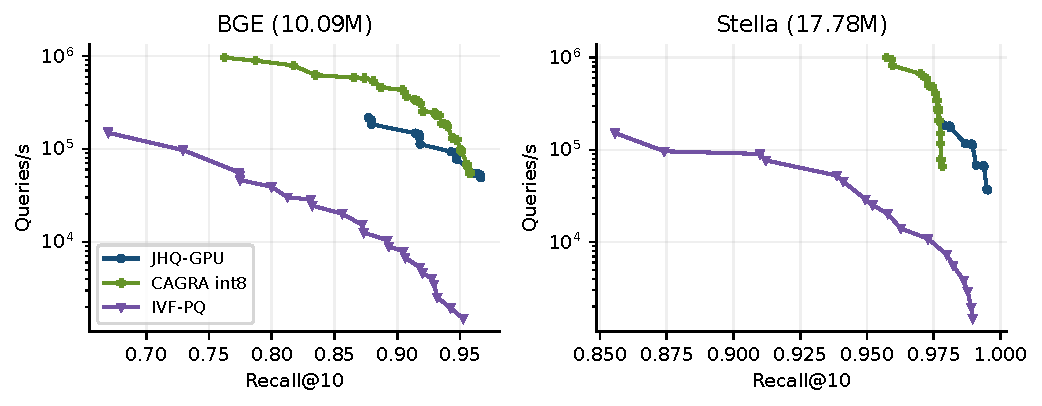
\includegraphics[width=\linewidth]{ch7/large_frontiers.pdf}
\caption{大数据集上的主机到主机前沿，包含 CAGRA int8 成功的隔离重跑。BGE 使用 1,000 条查询，Stella 使用 999 条。曲线端点是已测试网格的终点，不是方法的内在召回率上限。}
\label{fig:7-large}
\end{figure}

成功的隔离重跑显示，CAGRA int8 能在被测配置下装入 Stella。在 BGE 的共同采样目标 0.88/0.90/0.92/0.94/0.95 上，int8 约比 JHQ 快 $1.35$--$2.96\times$；在 int8 的最高实测召回率 0.9579 处，JHQ 插值 QPS 是 int8 的 $1.086\times$。因此，优势在高召回率末端附近反转。BGE/Stella 上，int8 的最高被测召回率为 0.9579/0.9783，JHQ 为 0.9663/0.9952，PQ 为 0.9525/0.9896。

Stella 上一个具体高端比较为：JHQ 在召回率 0.978679 时达到 185.4 kQPS，int8 在 0.978278 时为 66.3 kQPS，速率比为 $2.80\times$，两者召回率略有不同。这是一对明确的实测点，不是统一的匹配召回率优势：JHQ 很多更高召回率区间没有 int8 覆盖，而且其最高召回率点也以吞吐量换取质量。附录~\ref{app:reproducibility}记录修正运行的排除规则与测试程序诊断。

结果证明的是已测试规模和有价值的高召回率区间，而不是任意规模的可扩展性。最大已完成搜索是在单 GPU 上处理 17.78 百万个向量；本章没有多 GPU 实验，没有保持数据分布不变的扩展曲线，也没有接近显卡容量时的构建峰值证明。Stella 搜索使用实际的 999 条查询池。

\section{数值稳健性、异常与召回率归因}
\label{sec:7-8}

稳健性检查界定 RQ2 的精确性声明、RQ3 的风险评估与 RQ4 中较小的跨系统差距。

\subsection{质量分辨率与重复执行}

当 $k=10$、查询数为 1,000 时，多找回一个邻居会使总体 Recall@10 改变 $10^{-4}$；500 条留出查询时，分辨率为 $2\times10^{-4}$。Stella 的 499 查询划分略粗。这种离散分辨率不是不确定性区间，但有助于理解前面的小差异。第四位小数的变化可能只对应一两个结果槽位，而小的平均损失仍可能掩盖若干答案变化较大的查询。

重复计时调用也必须与重复索引构建分开。E1 解析器记录了 369 个标识符确定性标记为 false 的基线运行点：170 个 RaBitQ、80 个 IVF-PQ、68 个 CAGRA int8、50 个 CAGRA fp32，以及一个暴力搜索点。该标记可能包括并列结果的顺序变化，本身不意味着标识符集合变化或输出无效。没有测量点仅因这一标记而被丢弃。原始日志保留首次/末次召回率与集合、顺序诊断。JHQ 没有填写同样的基线标记，因此不能把它缺失该标记当作统一的跨方法确定性测试。较早 E1 报告的 401 使用的是 369 个 A 重复调用标记与 367 个 B 相对 A 不匹配标记的并集；其中 32 个点仅增加后一种标记。B 与 A 不一致是跨协议相等性检查，不等于重复调用 B 不确定。

五轮吞吐量摘要保留了固定构建内部的变化。最小值和最大值是描述性范围，不是置信区间，也不包括训练差异。因此，对两个 LUT 接近平手的例子、或 arXiv 与 RaBitQ 在召回率 0.97 处的小幅差距，不应赋予太大的解释权重。与对应阶段时间减少相匹配、幅度较大且能重复的收益，比单独一处微小前沿移动更能支持执行优化结论。

在各数据集 RaBitQ 配置间，“五轮最大值减最小值 / QPS 中位数”的中位数分别为：Vogue 3.79\%、arXiv 3.34\%、OpenAI-1536 2.87\%、OpenAI-3072 5.25\%。这些描述性波动与 Vogue 小幅领先的量级接近，而不是匹配比值的置信区间。原始调用轨迹也包含长调用，在原本较快的配置中偶有 30--60\,ms 观测。敏感性检验对 1,000 条查询的一次调用，按 $10^6/\operatorname{median}(\text{call latency in ms})$ 重算 QPS，以减小长调用的影响。召回率 0.97 处，得到的 JHQ/RaBitQ 比值为 1.063、0.995、1.118 和 1.100。三个有利方向与 arXiv 接近平手的格局保持，因此结果不只是长调用造成的。

\subsection{精确性必须限定到具体阶段}

几项不同声明必须区分。笛卡尔因子化在代数上保持已表示评分；打包加载保持逻辑编码值；采用完整键的局部保留和合并恢复已访问候选中的精确主码 top-$c$；共享界保持该选择目标；FP32 探针原语通过了合成与真实输入的等价检查。以上任何一项，都不等于在原始向量空间找到了精确最近邻。

lane 归约会改变舍入；主码截断边界的并列可能改变被精排的候选；最终选择对全部保留的精排评分进行精确选择，并按 ID 打破并列；相对原空间邻居的剩余误差可以来自此前阶段或已表示评分。归档中的 Vogue 跨版本差异说明，完整流水线的一致性需要独立检查。类似地，FP16 路由实验表明，几乎不变的平均召回率也不足以证明探针精确等价。因此，主要正确性结论都限定到实际测试过的阶段与输入覆盖。

召回率损失可能来自路由、主码筛选、残差评分或最终选择。增加探针扩大路由覆盖；增加 $\alpha$ 使更多主码候选进入残差评分；二者都不能恢复后续所有近似阶段丢失的信息。预算扫描固定索引和探针配置，直接测量改变保留候选数量的影响，却没有把每个遗漏邻居分解为唯一原因。完整逐查询归因需要在路由、主码保留和精排后分别检查真实邻居覆盖，并对同一候选集使用精确最终选择作为参考。本章所用实验尚未建立这种完整归因，因此不为未测量的损失来源分配百分比。

\subsection{研究发现的适用范围}

\Cref{tab:7-rq-answers} 收束 RQ1--RQ4 的证据链。结果支持少量面向表示的执行模式与工作负载相关精排工作量，并分别提供正确性、速度和质量证据。

\begin{table}[tbp]
\centering
\caption{本章证据支持的四个研究问题答案。}
\label{tab:7-rq-answers}
\small
\begin{tabularx}{\linewidth}{@{}l*{3}{>{\raggedright\arraybackslash}X}@{}}
\toprule
研究问题 & 证据 & 答案 & 边界 \\
\midrule
RQ1 & 冷构建、常驻组件、大规模搜索 & 单卡 17.78M 向量；20.44\,GiB；训练加添加 10.40\,s & 单次冷记录；未测构建峰值或多 GPU 扩展 \\
RQ2 & LUT、精排、扫描、共享界、探针配对测试 & 被测主码选择精确；批大小 8 调度为 $2.727\times$ & 并列与数值路径；全批次收益小得多 \\
RQ3 & 互斥查询划分、固定 64/100、oracle、枚举 & 平均 QPS 相对 64 胜 9/12，相对 100 胜 10/12 & 校准开销；最多 40/64 次相对 oracle 损失超标；未测漂移 \\
RQ4 & 六方法 E1 扫描、匹配召回率、显存 & 0.97 处三个领先，arXiv 接近平手；净分配低于 fp32 CAGRA & int8 在低召回率领先；端点和计时不确定性 \\
\bottomrule
\end{tabularx}
\end{table}

结论适用于平方 L2 的 top-10 搜索、记录查询池与被测 RTX 5090 环境。跨设备行为、变化查询、在线更新与开放到达服务延迟尚未测试。这些边界与正面结果共同呈现，而不是取代正面发现。

% Section structure adapted from 6.pdf; draft prompts are not thesis prose.
\chapter{Discussion, Limitations and Future Research}
\label{ch:discussion}
\draftnote{Synthesize supported findings, analyse two relevant negative designs, and state internal and external validity limits.}

\section{Three Cross-Layer Insights}
\label{sec:8-1}
\draftnote{Develop the supported links between representation and execution, parallelism and repeated work, and execution cost and the value of budget reduction.}

\section{Two Deep Negative-Result Case Studies}
\label{sec:8-2}
\draftnote{For two case studies, state hypothesis, alternatives, test conditions, observations, and stopping decision. Label isolated GPU, offline, estimated, and untested evidence.}

\section{Threats to Internal and External Validity}
\label{sec:8-3}
\draftnote{Write this section using the verified methods and evidence. State the relevant conditions and connect the argument to its research question.}

\section{Original Testable Research Directions}
\label{sec:8-4}
\draftnote{Write this section using the verified methods and evidence. State the relevant conditions and connect the argument to its research question.}

\section{Conditional Deployment Recommendation}
\label{sec:8-5}
\draftnote{Write this section using the verified methods and evidence. State the relevant conditions and connect the argument to its research question.}

% Section structure adapted from 6.pdf; draft prompts are not thesis prose.
\chapter{Conclusion}
\label{ch:conclusion}
\draftnote{Answer the research questions using only results already established. Do not introduce new measurements or contributions.}

\section{Answers to the Four Research Questions}
\label{sec:9-1}
\draftnote{Write this section using the verified methods and evidence. State the relevant conditions and connect the argument to its research question.}

\section{Closing Principle and Outlook}
\label{sec:9-2}
\draftnote{Write this section using the verified methods and evidence. State the relevant conditions and connect the argument to its research question.}


\clearpage
\phantomsection
\addcontentsline{toc}{chapter}{参考文献}
\bibliographystyle{plainnat}
\bibliography{references}

\appendix
\chapter{Reproducibility and Experiment Manifest}
\label{app:reproducibility}
\section{Source and Build Environment}
\draftnote{Record immutable source commits, compiler options, GPU and host
details, dependencies, and how the binaries were built. Distinguish the thesis
repository from the implementation repository.}
\section{Data and Trained States}
\draftnote{Document dataset identifiers, preprocessing, query and GT hashes,
split rules, trained-state cache identities, and exclusions.}
\section{Result-to-Figure Mapping}
\draftnote{Map every empirical figure to its raw files, analysis script,
configuration, metric definition, and reproduction command. Explain exactly
what cold construction includes.}

\chapter{Supplementary Results and Correctness Checks}
\label{app:supplementary}
\section{Complete Parameter Grids}
\draftnote{List method-specific tuning grids, invalid or unavailable settings,
and reasons for unattempted configurations.}
\section{Correctness and Numerical Checks}
\draftnote{Include reference comparisons for encoding, LUT factorisation,
primary selection, probe selection, and refinement. Separate numerical,
algorithmic, and memory-safety evidence.}
\section{Additional Results and Negative Designs}
\draftnote{Include secondary results with evidence status: integrated system,
isolated GPU measurement, offline replay, analytical estimate, or untested idea.}

\chapter{Contributions and Tool-Use Record}
\label{app:author-tools}
\draftnote{Use the form of disclosure required by Canvas. The tables below
are a record template, not an attestation that any particular verification
was performed. Replace all entries with a truthful account.}
\section{Contribution Record}
\begin{longtable}{@{}p{0.22\textwidth}p{0.34\textwidth}p{0.34\textwidth}@{}}
\toprule
Work component & Contributor and role & Supporting record \\
\midrule
\endhead
\textit{To complete} & \textit{To complete} & \textit{To complete} \\
\bottomrule
\end{longtable}
\section{Generative-AI Assistance}
\begin{longtable}{@{}p{0.19\textwidth}p{0.34\textwidth}p{0.37\textwidth}@{}}
\toprule
Tool and date & Purpose and scope & Prompt record and human review \\
\midrule
\endhead
\textit{To complete} & \textit{To complete} & \textit{To complete} \\
\bottomrule
\end{longtable}

\ifdraftthesis
  % Included only while \draftthesistrue. It is not thesis content.
\chapter{Template Examples --- Draft Only}
\label{app:template-examples}
This appendix demonstrates the available formatting. It is omitted when
\verb|\draftthesisfalse| is selected in \texttt{config/metadata.tex}.

\section{Citations and Cross-References}
Use \verb|\citet{jhq}| for a narrative citation: \citet{jhq}.
Use \verb|\citep{pq,cagra}| for a parenthetical citation \citep{pq,cagra}.
Examples: \cref{fig:example-pipeline,tab:example-manifest,eq:example-disagreement}.
The bibliography entries are copied from the existing ADC source; review their
metadata before submission.

\section{A Source-Native Diagram}
\begin{figure}[tbp]
\centering
\begin{tikzpicture}[
  node distance=5mm,
  stage/.style={draw=ThesisNavy,rounded corners=2pt,fill=ThesisNavy!4,
    minimum height=10mm,text width=26mm,align=center,font=\small},
  link/.style={-{Latex},draw=ThesisNavy}]
  \node[stage] (route) {IVF routing};
  \node[stage,right=of route] (screen) {Primary screening};
  \node[stage,right=of screen] (refine) {Residual refinement};
  \node[stage,right=of refine] (output) {Final top-$k$};
  \draw[link] (route) -- (screen);
  \draw[link] (screen) -- (refine);
  \draw[link] (refine) -- (output);
\end{tikzpicture}
\caption{Formatting example: a schematic query path. Replace or extend it
with the verified execution boundaries of the implementation.}
\label{fig:example-pipeline}
\end{figure}

% A real PDF figure can be inserted without copying any local absolute paths:
% \begin{figure}[tbp]
%   \centering
%   \includegraphics[width=\linewidth]{frontier.pdf}
%   \caption{State version, dataset, hardware, k, batch, timing boundary,
%     varied parameters, uncertainty, and interpolation when relevant.}
%   \label{fig:frontier}
% \end{figure}

\section{Tables}
\begin{table}[tbp]
\centering
\caption{Example manifest fields. This table contains no experimental results.}
\label{tab:example-manifest}
\begin{tabularx}{\linewidth}{@{}lX@{}}
\toprule
Field & What to record \\
\midrule
Source & Immutable commit and build configuration \\
Index & Trained-state identity and input hashes \\
Timing & Host-to-host or device-resident boundary \\
Quality & Metric, ground truth, and held-out split \\
Evidence & Raw log and analysis-script path \\
\bottomrule
\end{tabularx}
\end{table}

\section{Equations and Proofs}
\begin{equation}
 D(\alpha)=\sum_{q\in Q_s}
  \left[k-\left|R_\alpha(q)\cap R_{\max}(q)\right|\right].
 \label{eq:example-disagreement}
\end{equation}
The environments \texttt{definition}, \texttt{lemma}, \texttt{proposition},
and \texttt{proof} are available. For example:
\begin{definition}[Strict total ranking key]
A ranking key specifies how to order unequal scores and how to break ties.
\end{definition}
% \begin{proposition}[Descriptive title]
%   State the precise premises and claim here.
% \end{proposition}
% \begin{proof}
%   Give the argument, including floating-point and tie assumptions.
% \end{proof}

\section{Pseudocode and Code}
The table below gives a package-light pseudocode layout; replace its contents
with the actual method and keep correctness premises in the surrounding text.
\begin{table}[tbp]
\centering
\caption{Pseudocode layout example.}
\begin{tabularx}{\linewidth}{@{}rX@{}}
\toprule
Line & Operation \\
\midrule
1 & Read the input and validate the stated preconditions. \\
2 & Compute the intermediate result. \\
3 & Return the output and specify its semantics. \\
\bottomrule
\end{tabularx}
\end{table}
\begin{lstlisting}[language=C++,caption={Code-listing format example.}]
// Use only short excerpts that help explain a design.
// Keep full implementations in the reproducibility artifact.
void search();
\end{lstlisting}

\fi
\end{document}
